% Options for packages loaded elsewhere
\PassOptionsToPackage{unicode}{hyperref}
\PassOptionsToPackage{hyphens}{url}
\PassOptionsToPackage{dvipsnames,svgnames*,x11names*}{xcolor}
%
\documentclass[
]{book}
\usepackage{amsmath,amssymb}
\usepackage{lmodern}
\usepackage{ifxetex,ifluatex}
\ifnum 0\ifxetex 1\fi\ifluatex 1\fi=0 % if pdftex
  \usepackage[T1]{fontenc}
  \usepackage[utf8]{inputenc}
  \usepackage{textcomp} % provide euro and other symbols
\else % if luatex or xetex
  \usepackage{unicode-math}
  \defaultfontfeatures{Scale=MatchLowercase}
  \defaultfontfeatures[\rmfamily]{Ligatures=TeX,Scale=1}
\fi
% Use upquote if available, for straight quotes in verbatim environments
\IfFileExists{upquote.sty}{\usepackage{upquote}}{}
\IfFileExists{microtype.sty}{% use microtype if available
  \usepackage[]{microtype}
  \UseMicrotypeSet[protrusion]{basicmath} % disable protrusion for tt fonts
}{}
\makeatletter
\@ifundefined{KOMAClassName}{% if non-KOMA class
  \IfFileExists{parskip.sty}{%
    \usepackage{parskip}
  }{% else
    \setlength{\parindent}{0pt}
    \setlength{\parskip}{6pt plus 2pt minus 1pt}}
}{% if KOMA class
  \KOMAoptions{parskip=half}}
\makeatother
\usepackage{xcolor}
\IfFileExists{xurl.sty}{\usepackage{xurl}}{} % add URL line breaks if available
\IfFileExists{bookmark.sty}{\usepackage{bookmark}}{\usepackage{hyperref}}
\hypersetup{
  pdftitle={R Programming: Zero to Pro},
  pdfauthor={Yang Feng and Jianan Zhu},
  colorlinks=true,
  linkcolor=Maroon,
  filecolor=Maroon,
  citecolor=Blue,
  urlcolor=Blue,
  pdfcreator={LaTeX via pandoc}}
\urlstyle{same} % disable monospaced font for URLs
\usepackage{color}
\usepackage{fancyvrb}
\newcommand{\VerbBar}{|}
\newcommand{\VERB}{\Verb[commandchars=\\\{\}]}
\DefineVerbatimEnvironment{Highlighting}{Verbatim}{commandchars=\\\{\}}
% Add ',fontsize=\small' for more characters per line
\usepackage{framed}
\definecolor{shadecolor}{RGB}{248,248,248}
\newenvironment{Shaded}{\begin{snugshade}}{\end{snugshade}}
\newcommand{\AlertTok}[1]{\textcolor[rgb]{0.94,0.16,0.16}{#1}}
\newcommand{\AnnotationTok}[1]{\textcolor[rgb]{0.56,0.35,0.01}{\textbf{\textit{#1}}}}
\newcommand{\AttributeTok}[1]{\textcolor[rgb]{0.77,0.63,0.00}{#1}}
\newcommand{\BaseNTok}[1]{\textcolor[rgb]{0.00,0.00,0.81}{#1}}
\newcommand{\BuiltInTok}[1]{#1}
\newcommand{\CharTok}[1]{\textcolor[rgb]{0.31,0.60,0.02}{#1}}
\newcommand{\CommentTok}[1]{\textcolor[rgb]{0.56,0.35,0.01}{\textit{#1}}}
\newcommand{\CommentVarTok}[1]{\textcolor[rgb]{0.56,0.35,0.01}{\textbf{\textit{#1}}}}
\newcommand{\ConstantTok}[1]{\textcolor[rgb]{0.00,0.00,0.00}{#1}}
\newcommand{\ControlFlowTok}[1]{\textcolor[rgb]{0.13,0.29,0.53}{\textbf{#1}}}
\newcommand{\DataTypeTok}[1]{\textcolor[rgb]{0.13,0.29,0.53}{#1}}
\newcommand{\DecValTok}[1]{\textcolor[rgb]{0.00,0.00,0.81}{#1}}
\newcommand{\DocumentationTok}[1]{\textcolor[rgb]{0.56,0.35,0.01}{\textbf{\textit{#1}}}}
\newcommand{\ErrorTok}[1]{\textcolor[rgb]{0.64,0.00,0.00}{\textbf{#1}}}
\newcommand{\ExtensionTok}[1]{#1}
\newcommand{\FloatTok}[1]{\textcolor[rgb]{0.00,0.00,0.81}{#1}}
\newcommand{\FunctionTok}[1]{\textcolor[rgb]{0.00,0.00,0.00}{#1}}
\newcommand{\ImportTok}[1]{#1}
\newcommand{\InformationTok}[1]{\textcolor[rgb]{0.56,0.35,0.01}{\textbf{\textit{#1}}}}
\newcommand{\KeywordTok}[1]{\textcolor[rgb]{0.13,0.29,0.53}{\textbf{#1}}}
\newcommand{\NormalTok}[1]{#1}
\newcommand{\OperatorTok}[1]{\textcolor[rgb]{0.81,0.36,0.00}{\textbf{#1}}}
\newcommand{\OtherTok}[1]{\textcolor[rgb]{0.56,0.35,0.01}{#1}}
\newcommand{\PreprocessorTok}[1]{\textcolor[rgb]{0.56,0.35,0.01}{\textit{#1}}}
\newcommand{\RegionMarkerTok}[1]{#1}
\newcommand{\SpecialCharTok}[1]{\textcolor[rgb]{0.00,0.00,0.00}{#1}}
\newcommand{\SpecialStringTok}[1]{\textcolor[rgb]{0.31,0.60,0.02}{#1}}
\newcommand{\StringTok}[1]{\textcolor[rgb]{0.31,0.60,0.02}{#1}}
\newcommand{\VariableTok}[1]{\textcolor[rgb]{0.00,0.00,0.00}{#1}}
\newcommand{\VerbatimStringTok}[1]{\textcolor[rgb]{0.31,0.60,0.02}{#1}}
\newcommand{\WarningTok}[1]{\textcolor[rgb]{0.56,0.35,0.01}{\textbf{\textit{#1}}}}
\usepackage{longtable,booktabs,array}
\usepackage{calc} % for calculating minipage widths
% Correct order of tables after \paragraph or \subparagraph
\usepackage{etoolbox}
\makeatletter
\patchcmd\longtable{\par}{\if@noskipsec\mbox{}\fi\par}{}{}
\makeatother
% Allow footnotes in longtable head/foot
\IfFileExists{footnotehyper.sty}{\usepackage{footnotehyper}}{\usepackage{footnote}}
\makesavenoteenv{longtable}
\usepackage{graphicx}
\makeatletter
\def\maxwidth{\ifdim\Gin@nat@width>\linewidth\linewidth\else\Gin@nat@width\fi}
\def\maxheight{\ifdim\Gin@nat@height>\textheight\textheight\else\Gin@nat@height\fi}
\makeatother
% Scale images if necessary, so that they will not overflow the page
% margins by default, and it is still possible to overwrite the defaults
% using explicit options in \includegraphics[width, height, ...]{}
\setkeys{Gin}{width=\maxwidth,height=\maxheight,keepaspectratio}
% Set default figure placement to htbp
\makeatletter
\def\fps@figure{htbp}
\makeatother
\setlength{\emergencystretch}{3em} % prevent overfull lines
\providecommand{\tightlist}{%
  \setlength{\itemsep}{0pt}\setlength{\parskip}{0pt}}
\setcounter{secnumdepth}{5}
\usepackage{booktabs}
\usepackage{longtable}
\usepackage[bf,singlelinecheck=off]{caption}

\usepackage{Alegreya}
\usepackage[scale=.8]{sourcecodepro}

\usepackage{framed,color}
\definecolor{shadecolor}{RGB}{248,248,248}

\renewcommand{\textfraction}{0.05}
\renewcommand{\topfraction}{0.8}
\renewcommand{\bottomfraction}{0.8}
\renewcommand{\floatpagefraction}{0.75}

\renewenvironment{quote}{\begin{VF}}{\end{VF}}
\let\oldhref\href
\renewcommand{\href}[2]{#2\footnote{\url{#1}}}

\ifxetex
  \usepackage{letltxmacro}
  \setlength{\XeTeXLinkMargin}{1pt}
  \LetLtxMacro\SavedIncludeGraphics\includegraphics
  \def\includegraphics#1#{% #1 catches optional stuff (star/opt. arg.)
    \IncludeGraphicsAux{#1}%
  }%
  \newcommand*{\IncludeGraphicsAux}[2]{%
    \XeTeXLinkBox{%
      \SavedIncludeGraphics#1{#2}%
    }%
  }%
\fi

\usepackage{makeidx}
\makeindex

\urlstyle{tt}

\usepackage{amsthm}
\makeatletter
\def\thm@space@setup{%
  \thm@preskip=8pt plus 2pt minus 4pt
  \thm@postskip=\thm@preskip
}
\makeatother

\frontmatter
\usepackage{color}
\usepackage{framed}
\setlength{\fboxsep}{.8em}

\newenvironment{blackbox}{
  \definecolor{shadecolor}{rgb}{0, 0, 0}  % black
  \color{white}
  \begin{shaded}}
 {\end{shaded}}
\newenvironment{infobox}[1]
  {
  \begin{itemize}
  \renewcommand{\labelitemi}{
    \raisebox{-.7\height}[0pt][0pt]{
      {\setkeys{Gin}{width=3em,keepaspectratio}
        \includegraphics{pics/#1}}
    }
  }
  \setlength{\fboxsep}{1em}
  \begin{blackbox}
  \item
  }
  {
  \end{blackbox}
  \end{itemize}
  }
\ifluatex
  \usepackage{selnolig}  % disable illegal ligatures
\fi
\usepackage[]{natbib}
\bibliographystyle{apalike}

\title{R Programming: Zero to Pro}
\author{\href{https://yangfeng.hosting.nyu.edu/}{Yang Feng} and \href{https://yangfeng.hosting.nyu.edu/authors/jianan-zhu/}{Jianan Zhu}}
\date{2022-01-13}

\begin{document}
\maketitle

{
\hypersetup{linkcolor=}
\setcounter{tocdepth}{1}
\tableofcontents
}
\hypertarget{preface}{%
\chapter*{Preface}\label{preface}}
\addcontentsline{toc}{chapter}{Preface}

This book is for anyone who is interested in learning R and Data Science. It is designed for people with zero background in programming.

We also have a companion R package named \textbf{r02pro}, containing the data sets used as well as interactive exercises for each part.

\hypertarget{contributing-to-the-book}{%
\chapter*{Contributing to the Book}\label{contributing-to-the-book}}
\addcontentsline{toc}{chapter}{Contributing to the Book}

To improve the book, we would like to ask for your help.

\hypertarget{submitting-questions-or-feedback}{%
\subsection*{Submitting Questions or Feedback}\label{submitting-questions-or-feedback}}
\addcontentsline{toc}{subsection}{Submitting Questions or Feedback}

If you have any questions or feedback (including typos or grammar issues) about any materials in the book, we greatly appreciate if you can write to us at \href{mailto:r02pro007@gmail.com}{\nolinkurl{r02pro007@gmail.com}}. We will also add your name in the Acknowledgment section to show our gratitude.

\hypertarget{contributing-exercises}{%
\subsection*{Contributing Exercises}\label{contributing-exercises}}
\addcontentsline{toc}{subsection}{Contributing Exercises}

We warmly welcome everyone to help the book via contributing exercises for each section. Please make sure the exercise you are contributing only needs the knowledge up to the specific section number (it of course can use any knowledge of all sections up to the particular section) you would like to put the exercise into.

Please submit the proposed exercise(s) via the \href{https://docs.google.com/forms/d/e/1FAIpQLSckpcPZvRSr2vju-J2w8NhOx_oIyYtd8uuX0xqq_ThfRWMltw/viewform}{Google Form}.

Thanks a lot for your contribution.

\hypertarget{acknowledgement}{%
\chapter*{Acknowledgement}\label{acknowledgement}}
\addcontentsline{toc}{chapter}{Acknowledgement}

This book is the product of numerous collaborative efforts. Among all people, we would like to thank Dr.~Rebecca Betensky, Dr.~Rumi Chunara, and Dr.~Hai Shu, for the initial planning of the new courses GPH-GU 2183: Introduction to Statistical Programming in R and GPH-GU 2183: Intermediate Statistical Programming in R. In addition, we
are most grateful to the students in the course GPH-GU 2183: Introduction to Statistical Programming in R in Fall 2021 at New York University. The list of people that made contributions include Xiaofeng Yang (\href{https://github.com/well9801}{@well9801}), Neethu Grace Johnson (\href{https://github.com/neethujohnson01}{@neethujohnson01}), Yifan Lai (\href{https://github.com/Yifan-Lai}{@Yifan-Lai}), Ruiming Yu (\href{https://github.com/OmakaseMaster}{@OmakaseMaster}), Zhihao Chen (\href{https://github.com/edwardzchen}{@edwardzchen}), Fan Bi (\href{https://github.com/fanbithededenne}{@fanbithededenne}), Rebecca Yu (\href{https://github.com/rjy2107}{@rjy2107}), Ting Lu (\href{https://github.com/tinglusince}{@tinglusince}), Yang Yang (\href{https://github.com/YoArtemis}{@YoArtemis}), Jian Li (\href{https://github.com/kegemor}{@kegemor}), Grace Lin (\href{https://github.com/gracexlyhl}{@gracexlyhl}), Xin Chen (\href{https://github.com/zoexinchen}{@zoexinchen}), Wanyu Hua (\href{https://github.com/hiWanyu}{@hiWanyu})

\hypertarget{building-environment}{%
\chapter*{Building Environment}\label{building-environment}}
\addcontentsline{toc}{chapter}{Building Environment}

The R session information when compiling this book is shown below.

\begin{Shaded}
\begin{Highlighting}[]
\FunctionTok{sessionInfo}\NormalTok{()}
\CommentTok{\#\textgreater{} R version 4.0.4 (2021{-}02{-}15)}
\CommentTok{\#\textgreater{} Platform: x86\_64{-}apple{-}darwin17.0 (64{-}bit)}
\CommentTok{\#\textgreater{} Running under: macOS Big Sur 10.16}
\CommentTok{\#\textgreater{} }
\CommentTok{\#\textgreater{} Matrix products: default}
\CommentTok{\#\textgreater{} BLAS:   /Library/Frameworks/R.framework/Versions/4.0/Resources/lib/libRblas.dylib}
\CommentTok{\#\textgreater{} LAPACK: /Library/Frameworks/R.framework/Versions/4.0/Resources/lib/libRlapack.dylib}
\CommentTok{\#\textgreater{} }
\CommentTok{\#\textgreater{} locale:}
\CommentTok{\#\textgreater{} [1] en\_US.UTF{-}8/en\_US.UTF{-}8/en\_US.UTF{-}8/C/en\_US.UTF{-}8/en\_US.UTF{-}8}
\CommentTok{\#\textgreater{} }
\CommentTok{\#\textgreater{} attached base packages:}
\CommentTok{\#\textgreater{} [1] stats     graphics  grDevices utils     datasets  methods   base     }
\CommentTok{\#\textgreater{} }
\CommentTok{\#\textgreater{} other attached packages:}
\CommentTok{\#\textgreater{} [1] dplyr\_1.0.2}
\CommentTok{\#\textgreater{} }
\CommentTok{\#\textgreater{} loaded via a namespace (and not attached):}
\CommentTok{\#\textgreater{}  [1] rstudioapi\_0.13   knitr\_1.36        magrittr\_2.0.1    hms\_0.5.3        }
\CommentTok{\#\textgreater{}  [5] tidyselect\_1.1.0  R6\_2.5.0          rlang\_0.4.10      stringr\_1.4.0    }
\CommentTok{\#\textgreater{}  [9] tools\_4.0.4       xfun\_0.23         htmltools\_0.5.1.1 ellipsis\_0.3.1   }
\CommentTok{\#\textgreater{} [13] yaml\_2.2.1        digest\_0.6.27     tibble\_3.0.4      lifecycle\_0.2.0  }
\CommentTok{\#\textgreater{} [17] crayon\_1.3.4      bookdown\_0.24     purrr\_0.3.4       readr\_1.4.0      }
\CommentTok{\#\textgreater{} [21] vctrs\_0.3.5       glue\_1.4.2        evaluate\_0.14     rmarkdown\_2.11   }
\CommentTok{\#\textgreater{} [25] stringi\_1.5.3     compiler\_4.0.4    pillar\_1.4.7      generics\_0.1.0   }
\CommentTok{\#\textgreater{} [29] pkgconfig\_2.0.3}
\end{Highlighting}
\end{Shaded}

In the book, package names are in \textbf{bold} text (e.g., \textbf{r02pro}), and inline codes and functions are formatted in a typewriter font (e.g.~\texttt{1\ +\ 2}, \texttt{r02pro()}). We always add parentheses after a function name (e.g.~\texttt{r02pro()}).

\hypertarget{introduction}{%
\chapter{Introduction}\label{introduction}}

This chapter begins with the installation of R, RStudio, and R Packages in Section \ref{Installation}, shows how to use R as a fancy calculator in Section \ref{Calculator}, followed by object assignments in Section \ref{Object-Assignment}.

\hypertarget{Installation}{%
\section{Installation of R, RStudio and R Packages}\label{Installation}}

\hypertarget{download-and-install}{%
\subsection{Download and Install}\label{download-and-install}}

As the first step, you need to download R and RStudio, whose links are as follows. For both software, you need to choose the version that corresponds to your operating system.

Download R: \url{https://cloud.r-project.org/}

Download RStudio: \url{https://rstudio.com/products/rstudio/download/\#download}

RStudio is an \emph{Integrated Development Environment} for R, which is powerful yet easy to use. Throughout this book, you will use RStudio instead of R to learn R programming. Without further ado, let's start with a quick tour of RStudio.

\hypertarget{rstudio-interface}{%
\subsection{RStudio Interface}\label{rstudio-interface}}

After opening RStudio for the first time, you may find that the font and button size is a bit small. Let's see how to customize the appearance.

\textbf{\emph{a. Customize appearance}}

On the RStudio menu bar, you can click \emph{Tools}, and then click on \emph{Global Options} as shown below.

\begin{figure}

{\centering 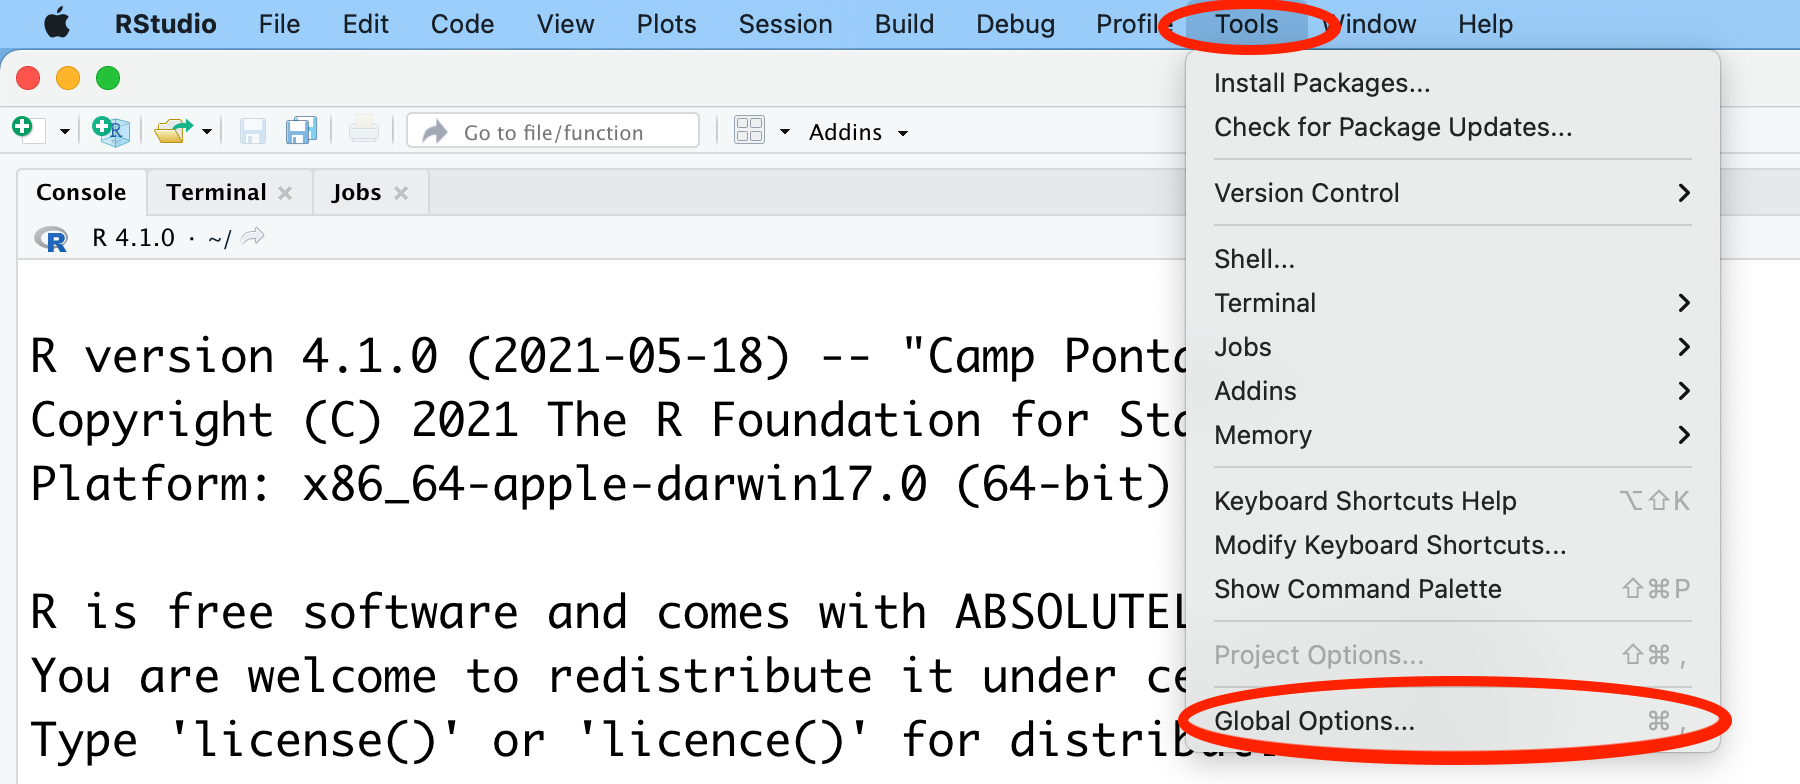
\includegraphics[width=0.9\linewidth]{pics/1font} 

}

\caption{Global Options}\label{fig:font}
\end{figure}

Then, you will see a window popping up like Figure \ref{fig:size}. After clicking on \emph{Appearance}, you can see several drop-down menus including \emph{Zoom} and \emph{Editor font size} among other choices shown.

\begin{itemize}
\item
  \emph{Zoom} controls the overall scale for all elements in the RStudio interface, including the sizes of the menu, buttons, as well as fonts.
\item
  \emph{Editor font size} controls the size of the font only in the code editor.
\end{itemize}

Once done customizing the appearance, you need to click on \emph{Apply} to save the adjustments.

\begin{figure}

{\centering 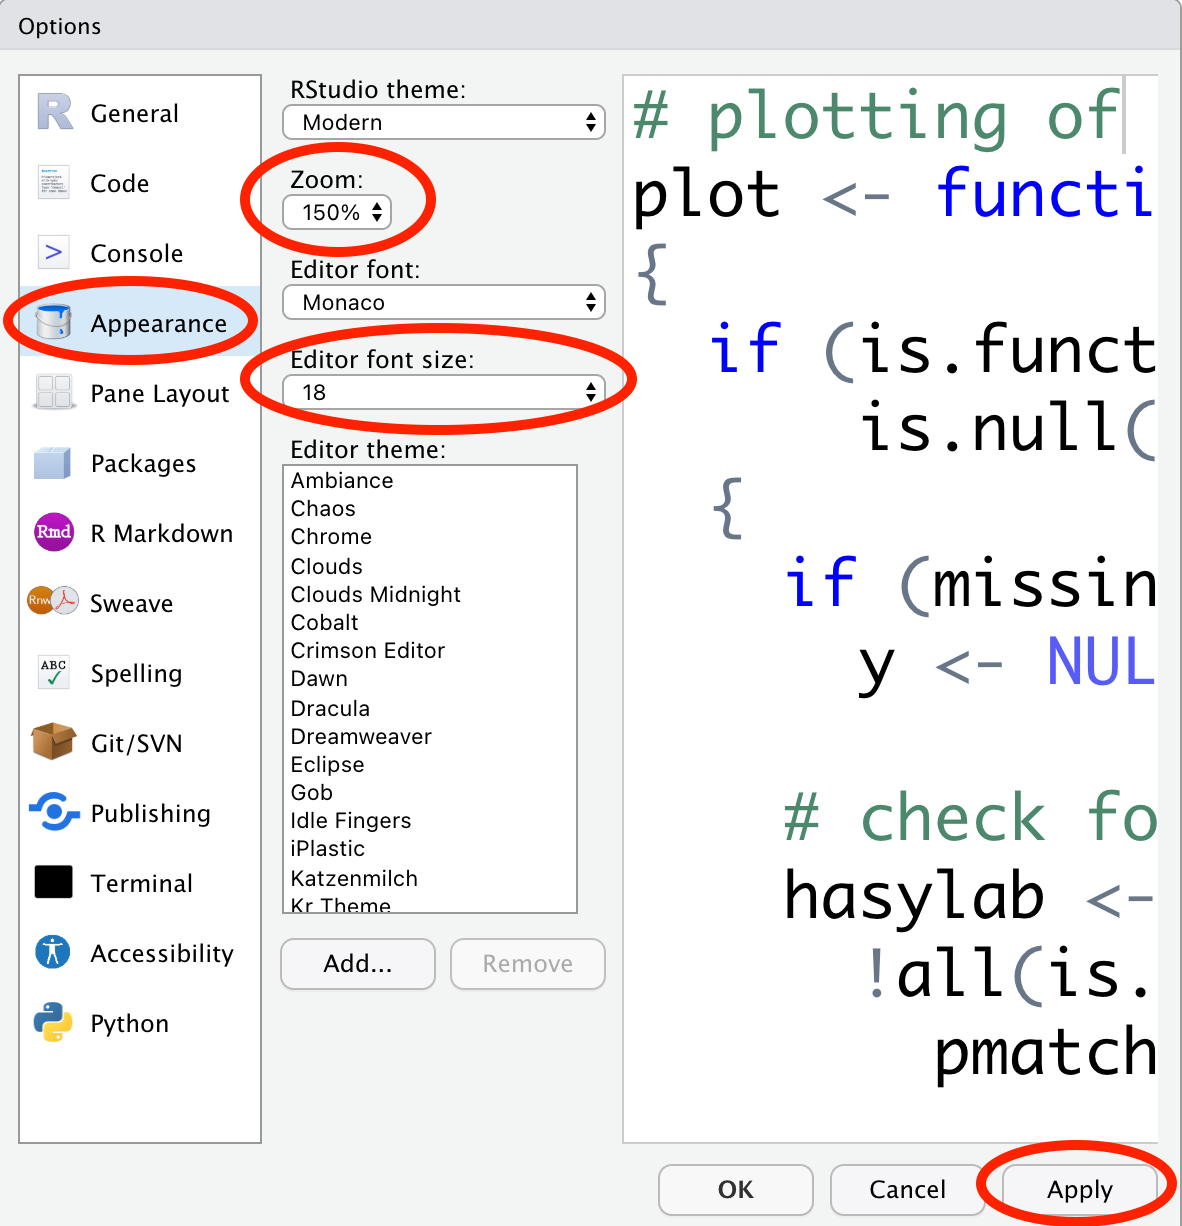
\includegraphics[width=0.7\linewidth]{pics/1size} 

}

\caption{Zoom and Editor font size}\label{fig:size}
\end{figure}

Here, we change the \emph{Zoom} to 150\% and set the \emph{Editor font size} to 18.

\textbf{\emph{b. Four panels of RStudio}}

Now, the RStudio interface is clearer with a bigger font size. Although RStudio has four panels, not all of them are visible to us at the beginning (Figure \ref{fig:open}).

\begin{figure}

{\centering 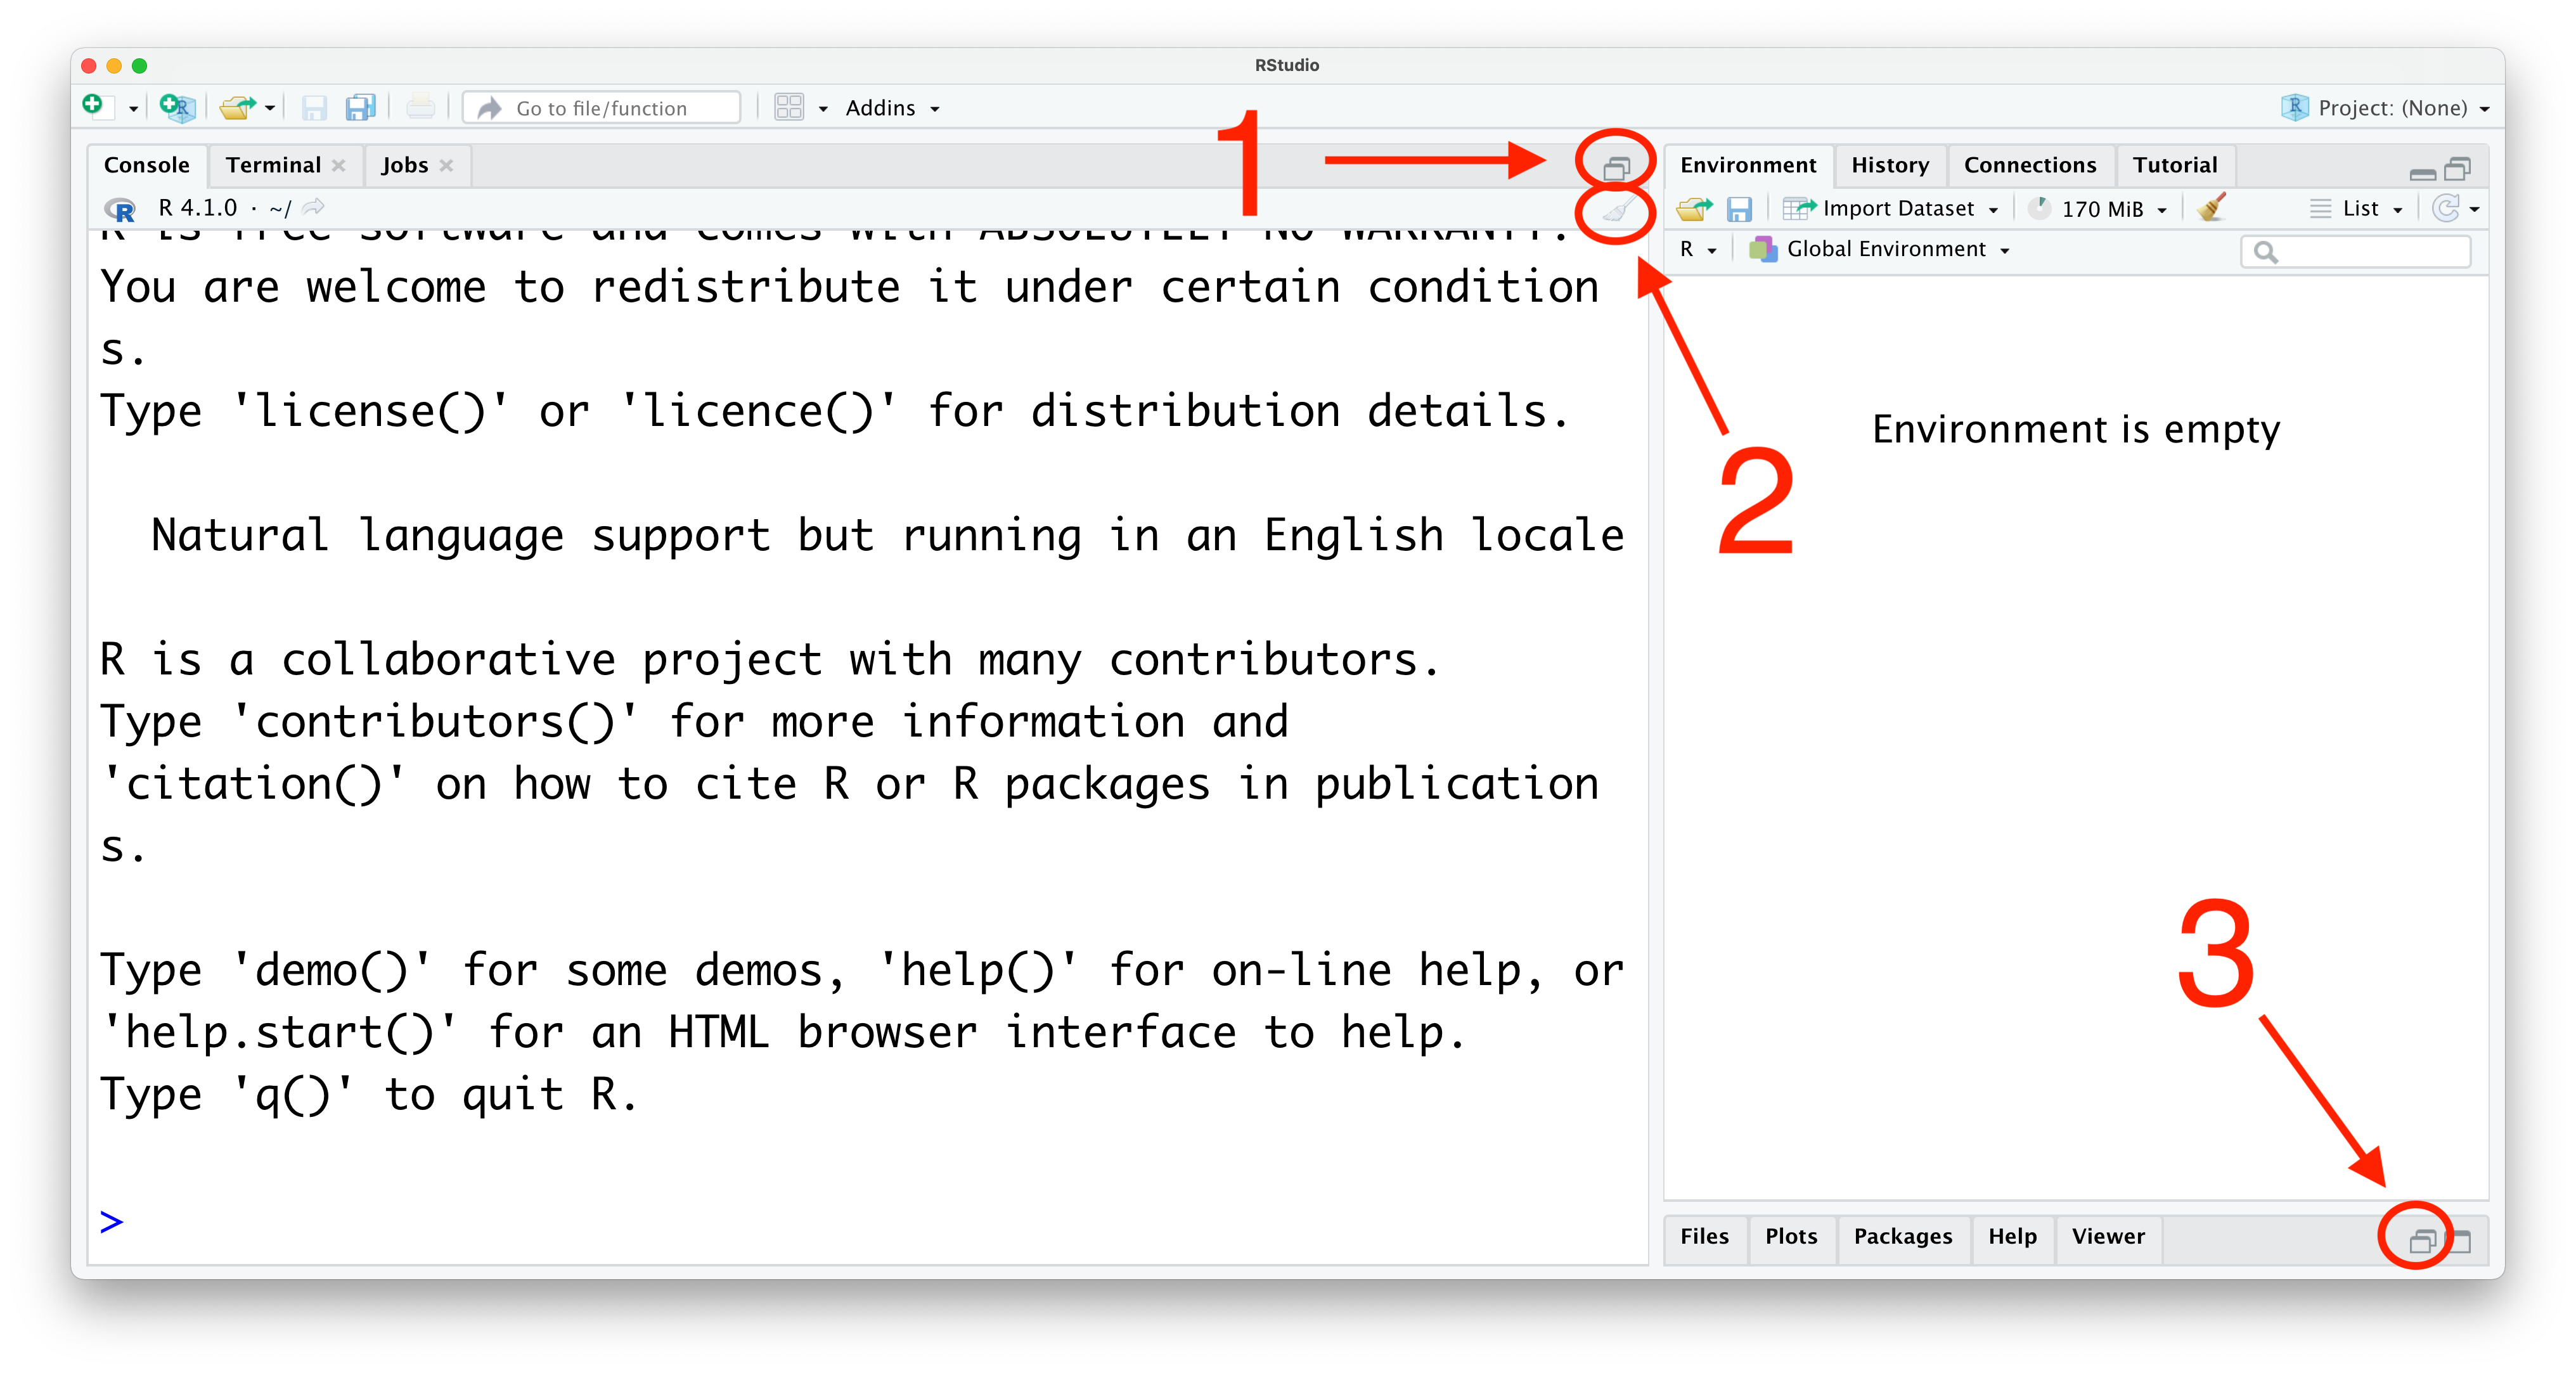
\includegraphics[width=1\linewidth]{pics/1open} 

}

\caption{Unfold panels}\label{fig:open}
\end{figure}

In Figure \ref{fig:open}, we have labeled three useful buttons as 1, 2, and 3. By clicking buttons 1 and 3, you can reveal the two hidden panels.

\begin{infobox}{caution}
Note that you may see different panels hidden when you open RStudio for the first time, depending on the RStudio version. However, you can always reveal the hidden panels by clicking the corresponding buttons like Buttons 1 and 3 in Figure \ref{fig:open}.

\end{infobox}

By clicking button 2, we can clear the content in the bottom left panel (Panel 2 in Figure \ref{fig:four}) as shown in the following figure.

\begin{figure}

{\centering 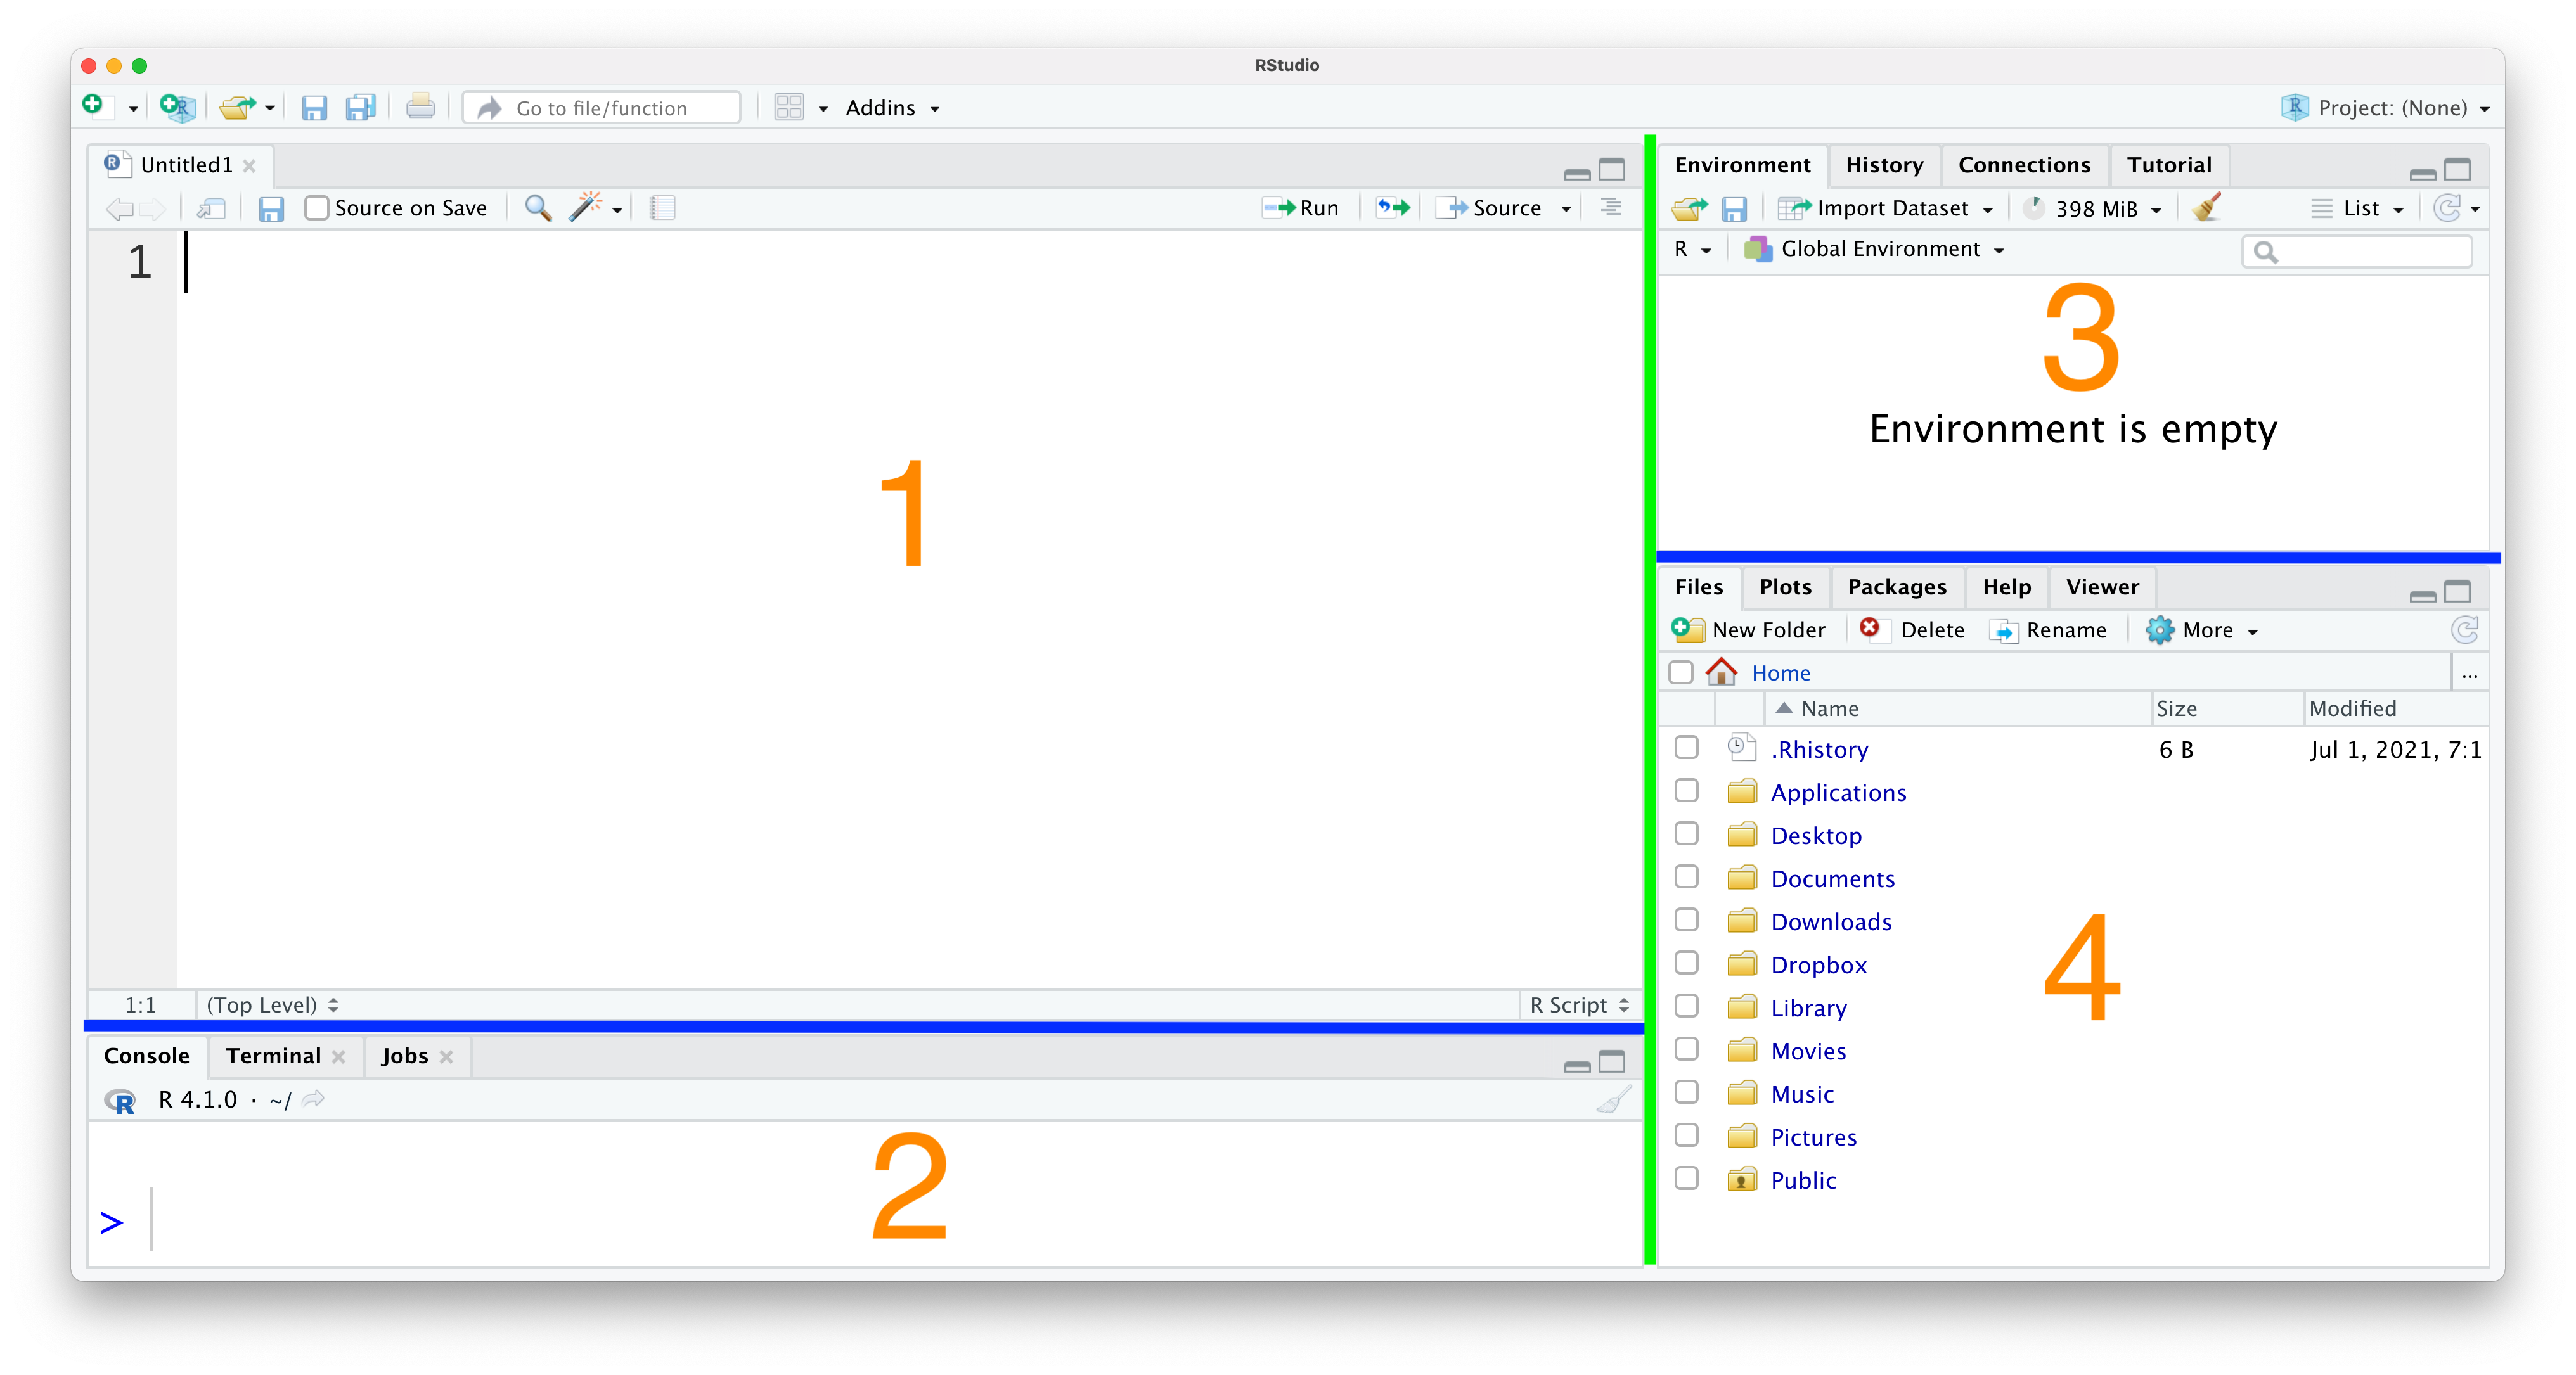
\includegraphics[width=1\linewidth]{pics/1four} 

}

\caption{Four panels}\label{fig:four}
\end{figure}

Now, let's take a close look at all four panels, which are labeled as 1-4 in Figure \ref{fig:four}. You can change the size of each panel by dragging the two blue slides \emph{up} or \emph{down} and the green slide \emph{left} or \emph{right}.

\begin{itemize}
\item
  Located to the left of the green line, Panels 1 and 2 together compose the \textbf{Code Area}. We will introduce them in the following parts of this section.
\item
  Located to the right of the green line, Panels 3 and 4 together make up the \textbf{R Support Area}. We will introduce these two panels in later sections.
\end{itemize}

\textbf{\emph{c.~Console}}

Firstly, we will introduce panel 2 in Figure \ref{fig:four}, which is usually called the \textbf{Console}. The console window is the place for you to type in codes (i.e.~the things you want R to do) and you will get the results immediately once you run the codes.

By clicking the mouse on the line after the \texttt{\textgreater{}} symbol, you can see a blinking cursor, indicating that R is ready to accept codes. Let's type \texttt{1\ +\ 2} and press \emph{Return} (on Mac) or \emph{Enter} (on Windows).

\begin{infobox}{caution}
It is a good habit to add spaces around an operator to increase the readability of the code.

\end{infobox}

\begin{figure}

{\centering 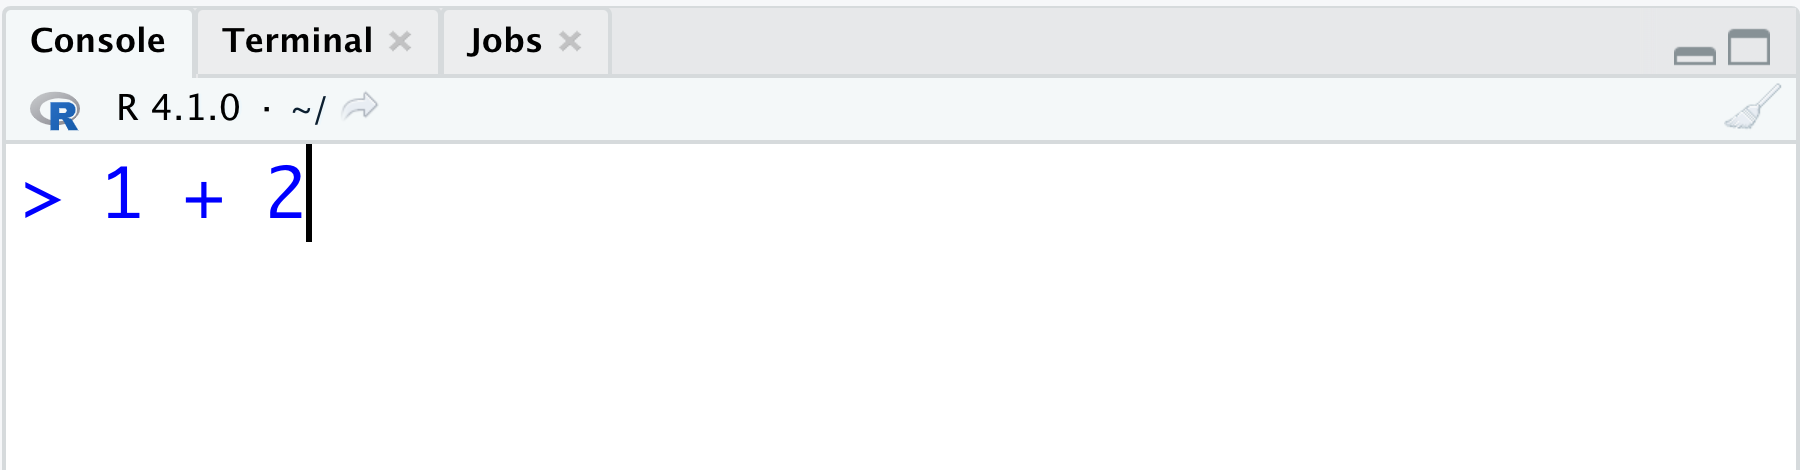
\includegraphics[width=0.7\linewidth]{pics/1code} 

}

\caption{Writing code in the console}\label{fig:code}
\end{figure}

\begin{figure}

{\centering 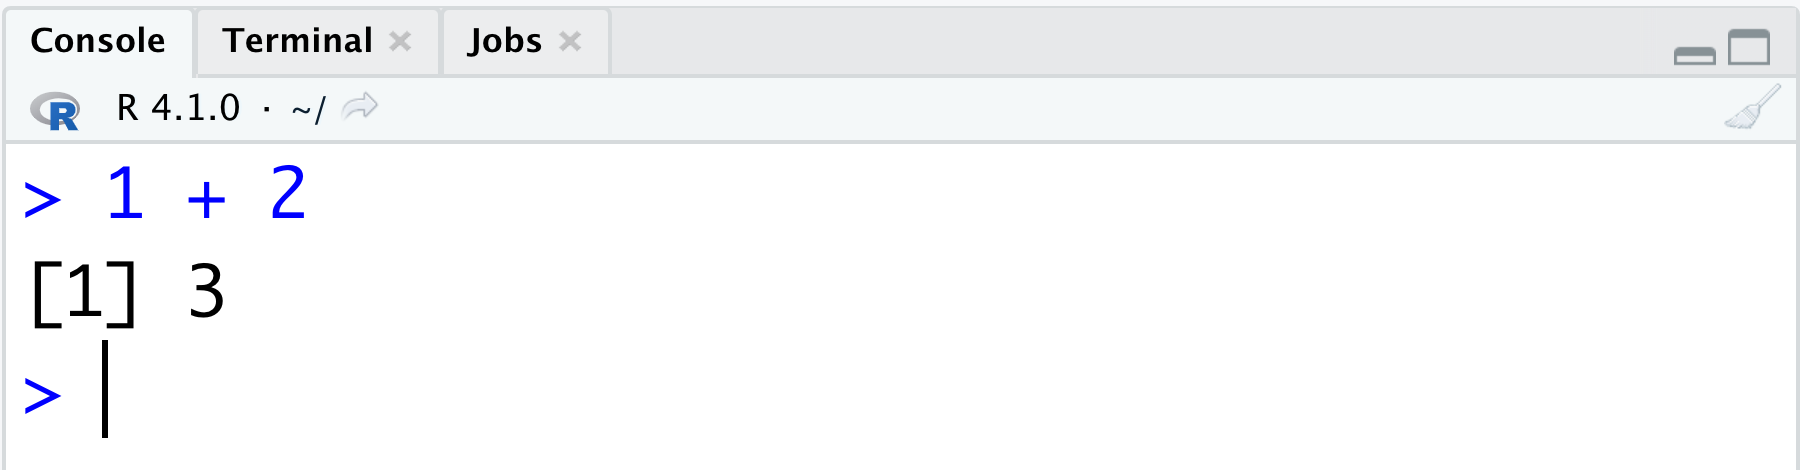
\includegraphics[width=0.7\linewidth]{pics/1answer} 

}

\caption{R code(2)}\label{fig:answer}
\end{figure}

Hooray! You have successfully run the first piece of R code and gotten the correct answer 3. Note that the blinking cursor now appears on the next line, ready to accept a new line of code.

\begin{infobox}{caution}
The curious you may found that there is a \texttt{{[}1{]}} showing before the result \texttt{3}. In fact, the \texttt{{[}1{]}} is an index indicator, showing the next element has an index of 1 in this particular object. We will revisit this point when we introduce vectors in the beginning of Chapter \ref{r-objects} .

\end{infobox}

Although the console may work well for some quick calculations, you need to resort to panel 1 in Figure \ref{fig:four} (known as the \textbf{Editor}) to save our work and run multiple lines of code at once.

\textbf{\emph{d.~Editor}}

The \textbf{Editor} panel is the go-to place to write complicated R codes, which you can save as R files for repeated use in the future. Several kinds of files are available in RStudio. In particular, \textbf{R script}, \textbf{R Markdown}, and \textbf{R Notebook} are the three most common file formats. In order to let you get started better, we will start with R script since this is the simplest file format in R. In Chapter 12 and ??, we will introduce R Markdown and R Notebook in detail.

In the editor panel, you may notice that RStudio has created a file by default (Figure \ref{fig:P1}). The default file RStudio provided is \textbf{R script}.

\begin{figure}

{\centering 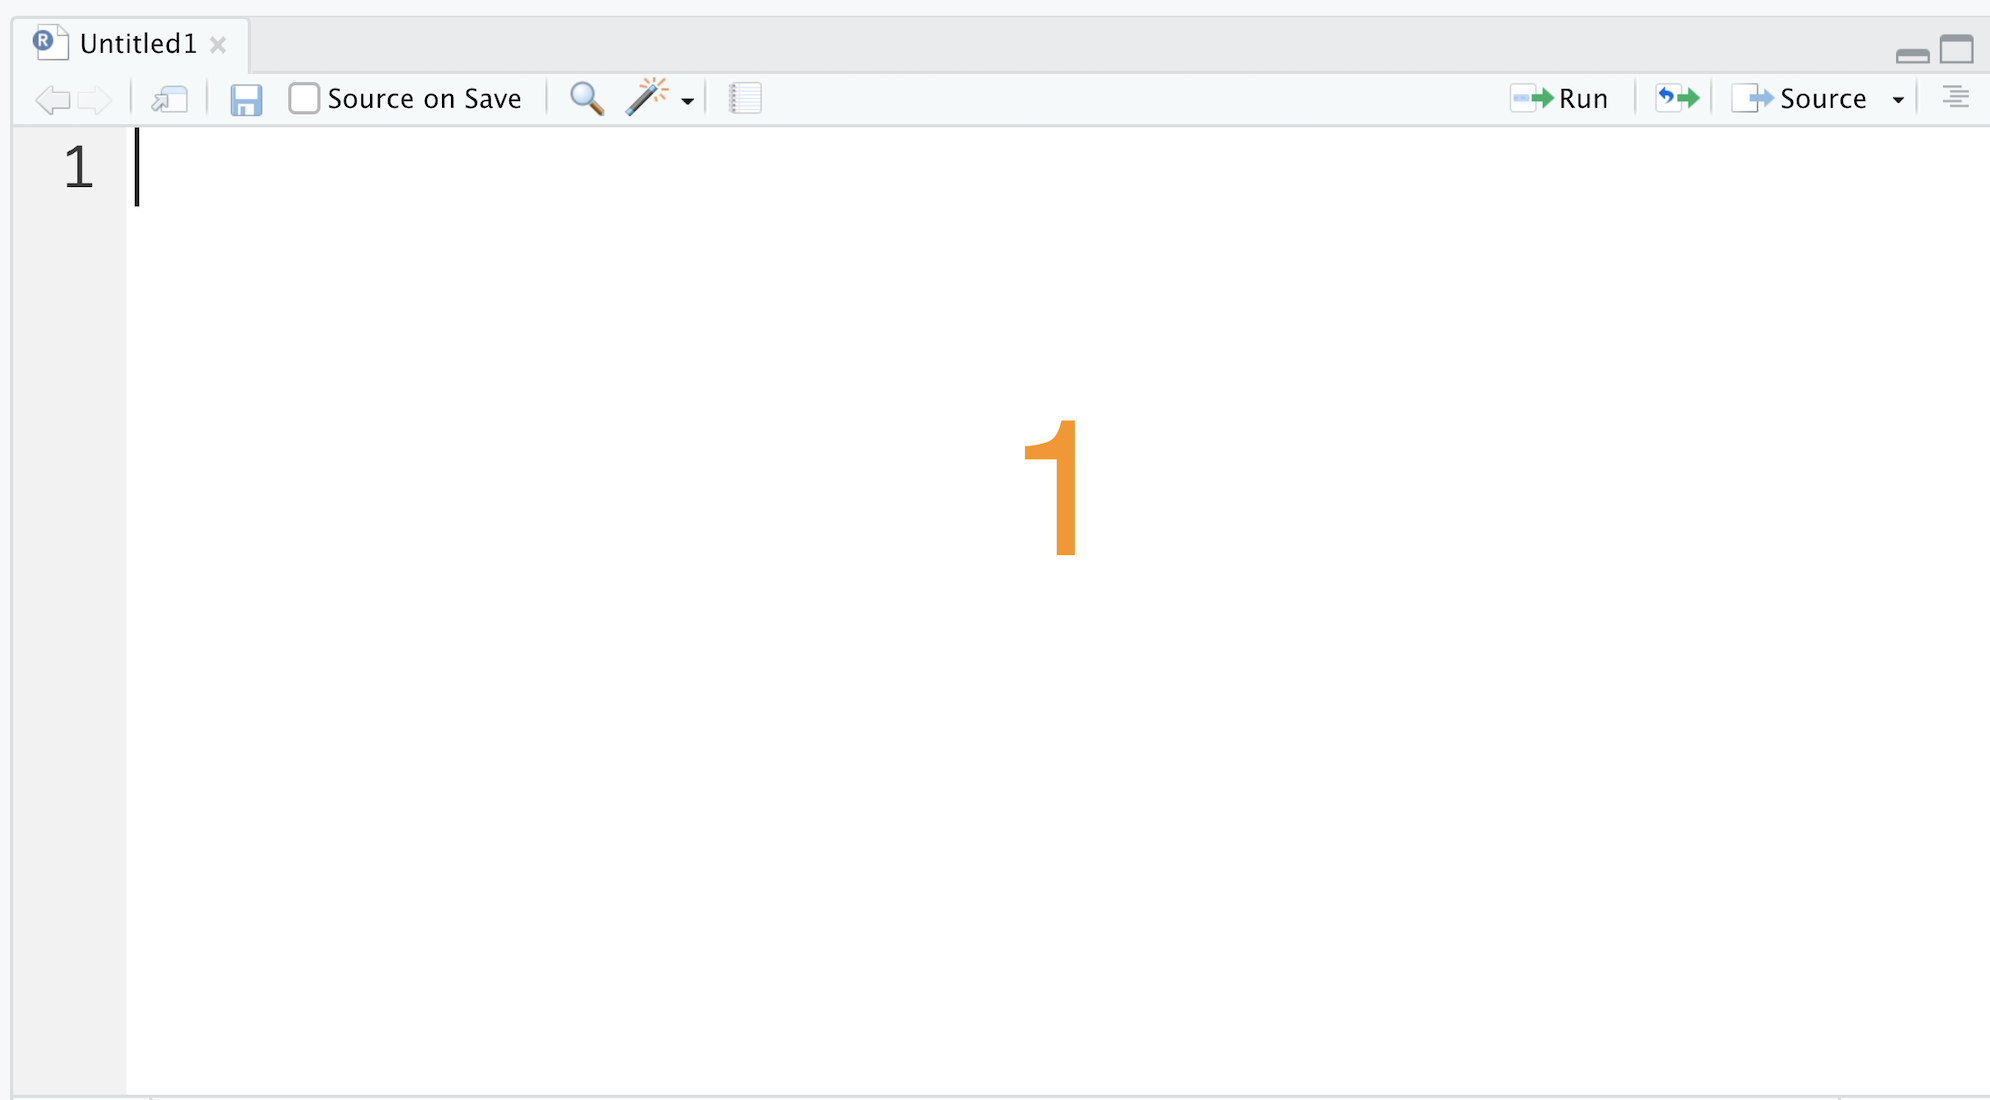
\includegraphics[width=0.7\linewidth]{pics/1P1} 

}

\caption{R script}\label{fig:P1}
\end{figure}

Next, we will introduce how to run codes in scripts. Let's go to the editor and type \texttt{1\ +\ 2}. To run this line of code, you can select this line of code and click the \emph{Run} button. The keyboard shortcut of running this line of code is Cmd+Return on Mac or Ctrl+Enter on Windows. RStudio will then send the line of code to the console and execute the code.

\begin{figure}

{\centering 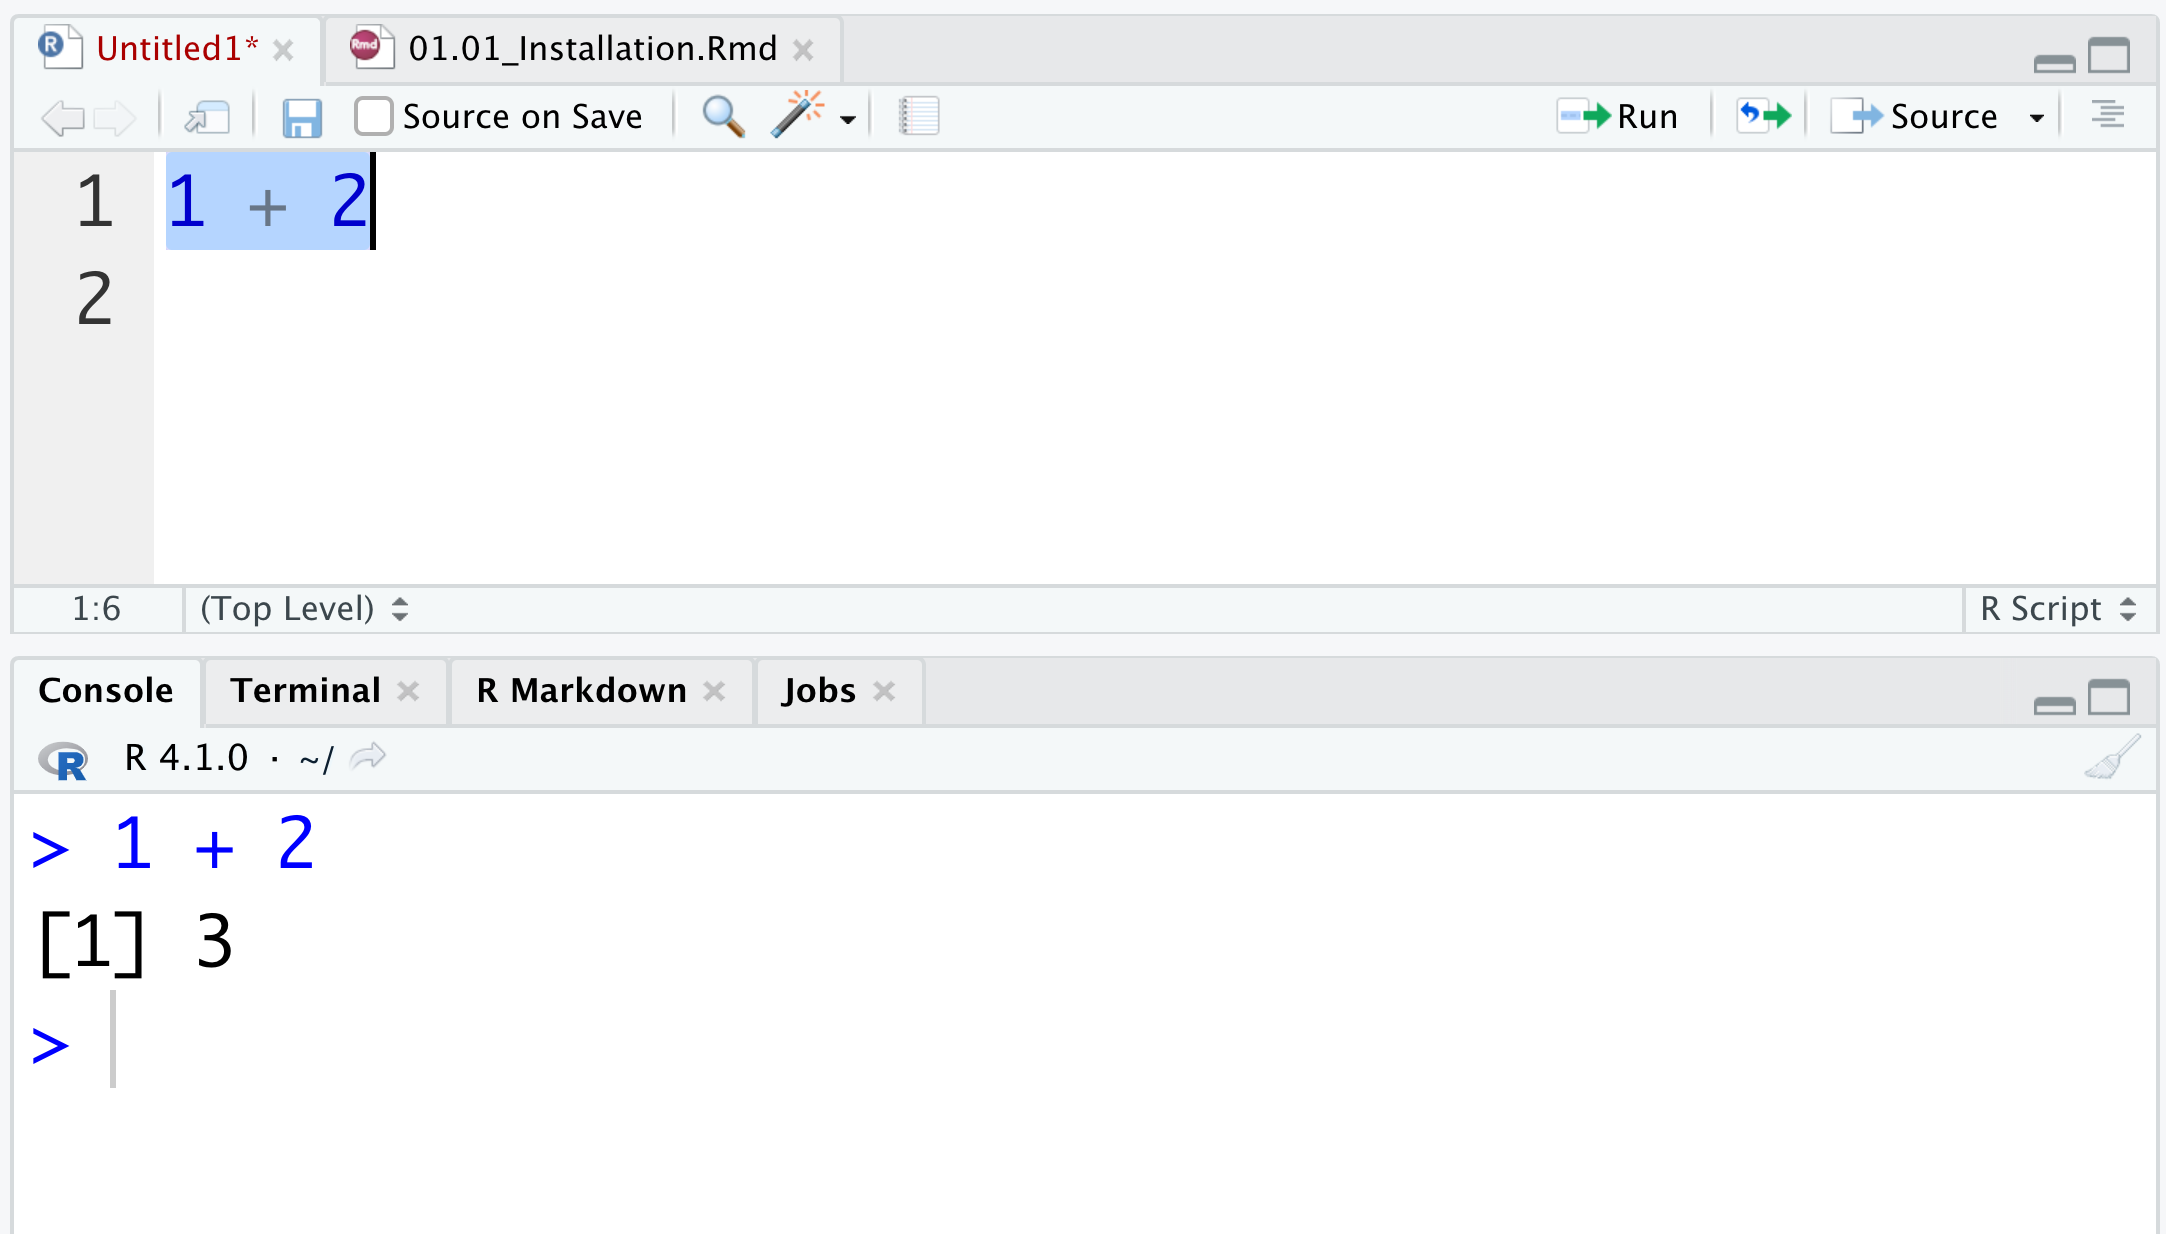
\includegraphics[width=0.7\linewidth]{pics/1run} 

}

\caption{Run codes in script (I)}\label{fig:run}
\end{figure}

You can also run multiple lines of code by selecting the lines and clicking the \emph{Run} button or using the keyboard shortcut. (Figure \ref{fig:mcodes})

\begin{figure}

{\centering 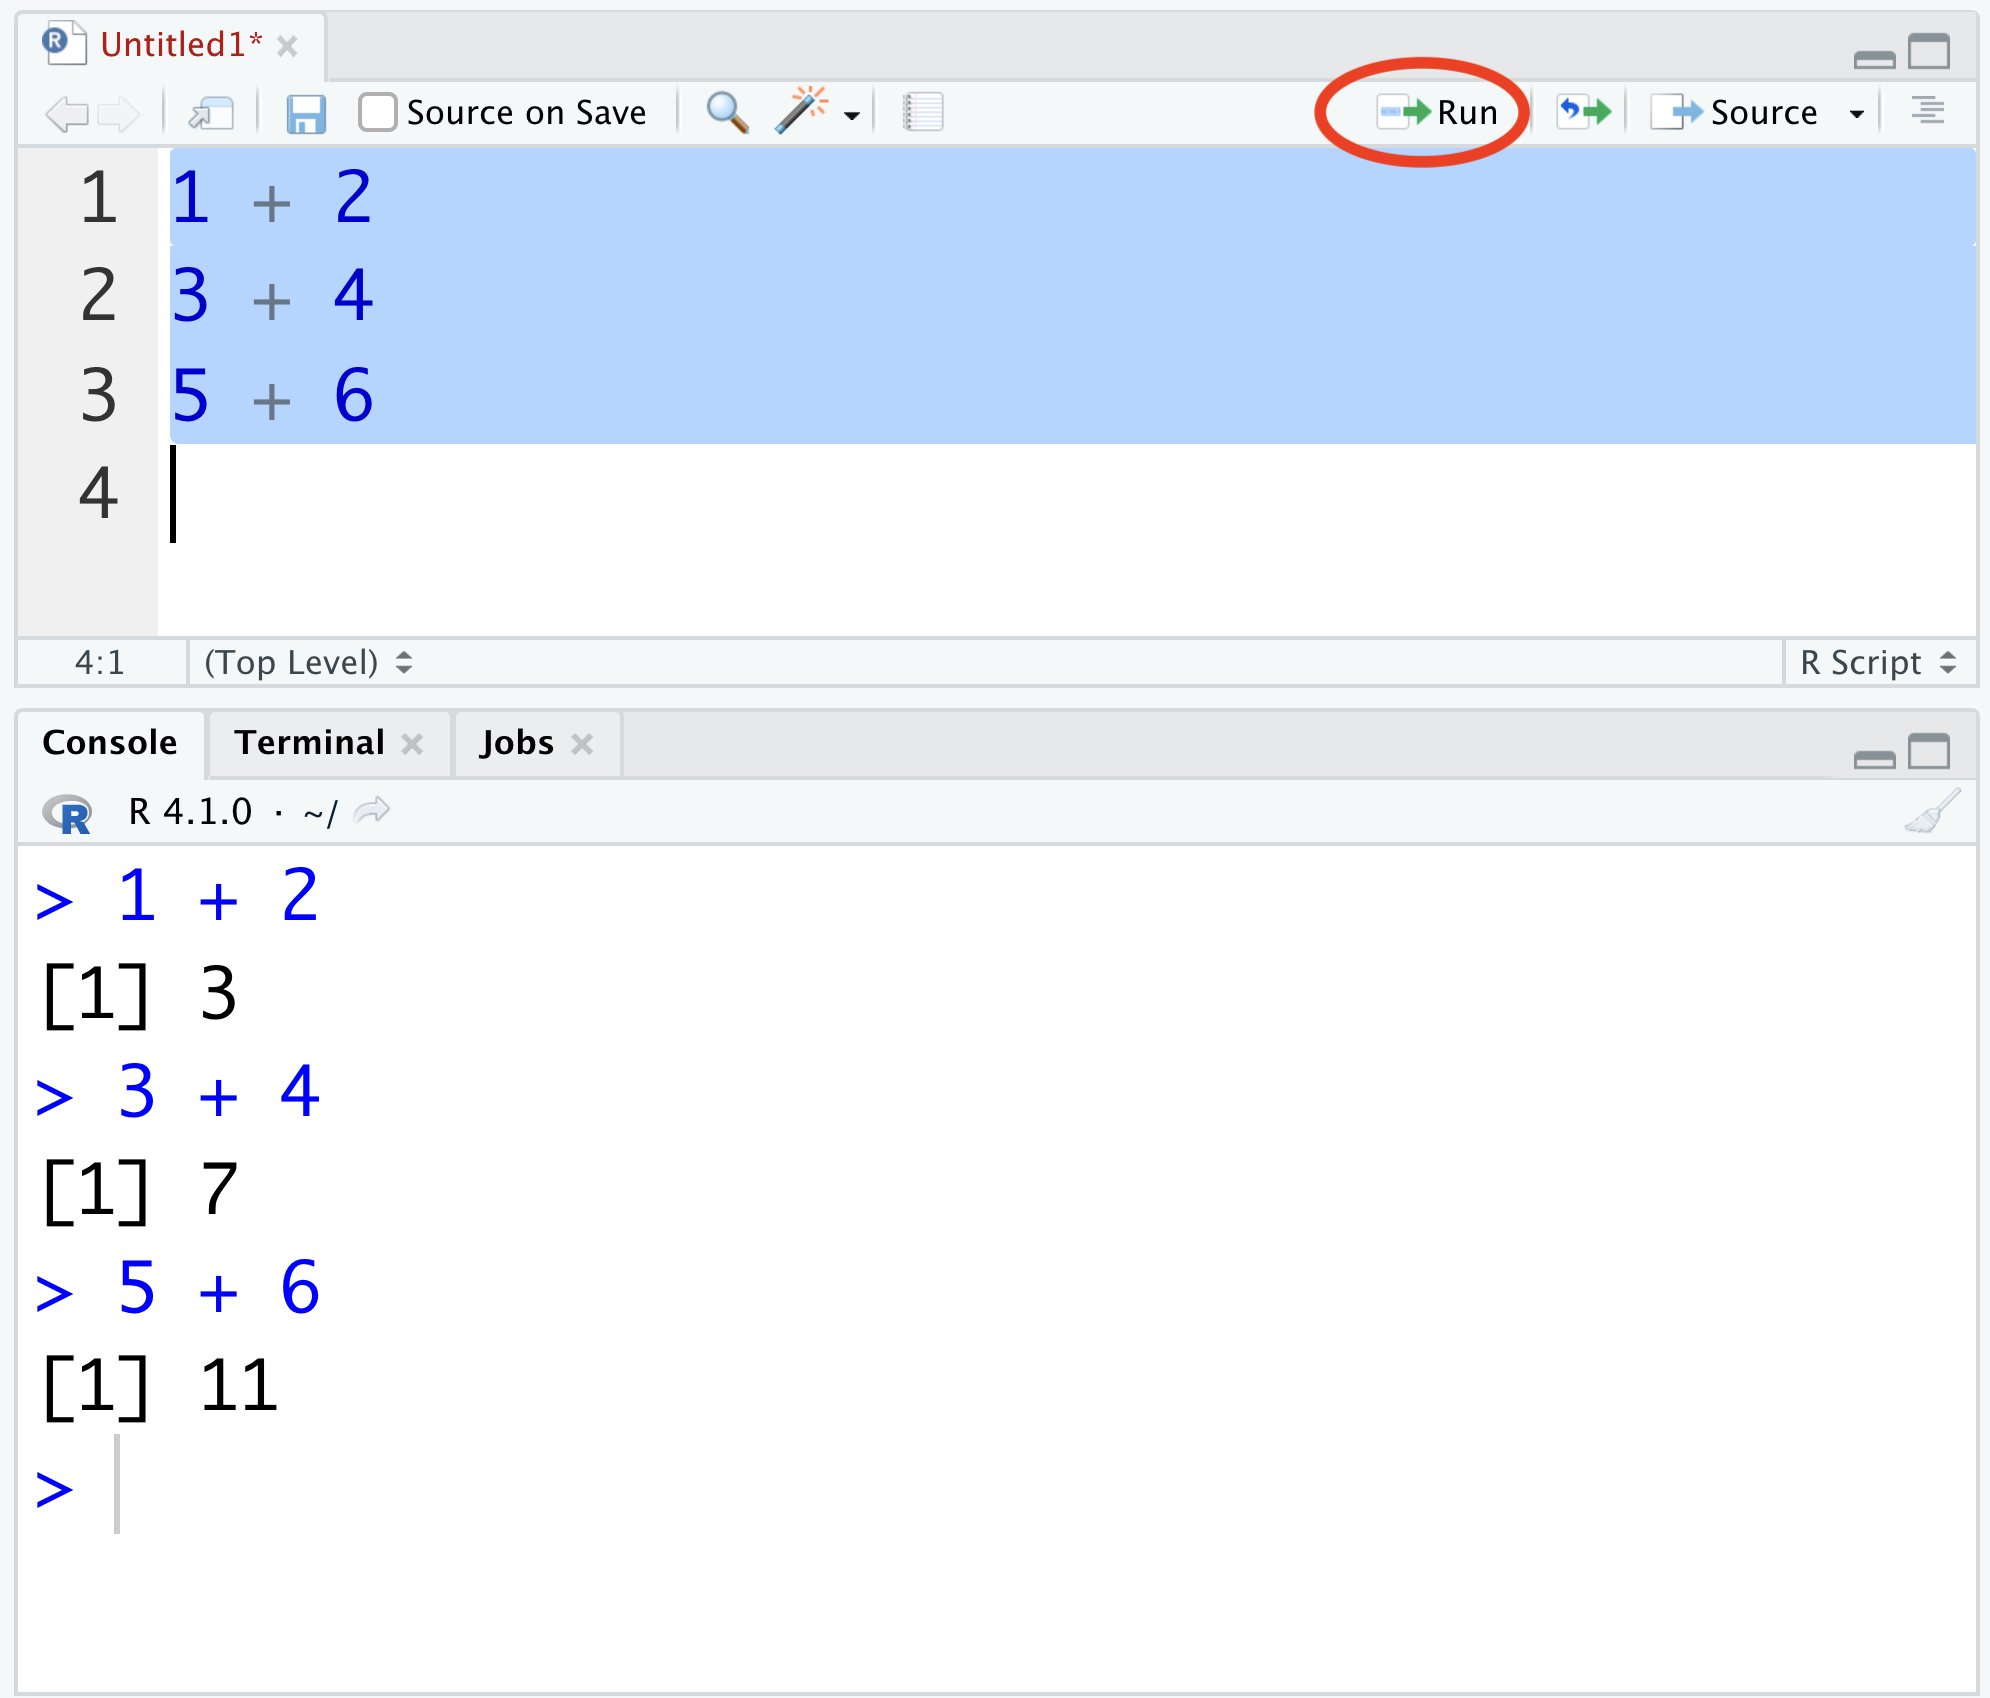
\includegraphics[width=0.7\linewidth]{pics/1mcodes} 

}

\caption{Run codes in script (II)}\label{fig:mcodes}
\end{figure}

Here, three lines of codes are selected. After running these three lines of code together, you can see that the console executes each line of code and you will get the corresponding answer one by one. Therefore, you can write any number of lines of codes in the script, and you can get the answer of each line in the console.

After finishing writing codes in the editor, there may be hundreds or more lines of codes in the script. Now, you may wonder if you need to write these codes again when you want to use the same codes next time. The answer is absolutely NO!!! One of the most important features of R files is that R files can be saved for future use. So do R scripts! To do that, you can click the \emph{Save} button as shown in Figure \ref{fig:save1}. The keyboard shortcut of saving files is Cmd+S on Mac or Ctrl+S on Windows.

\begin{figure}

{\centering 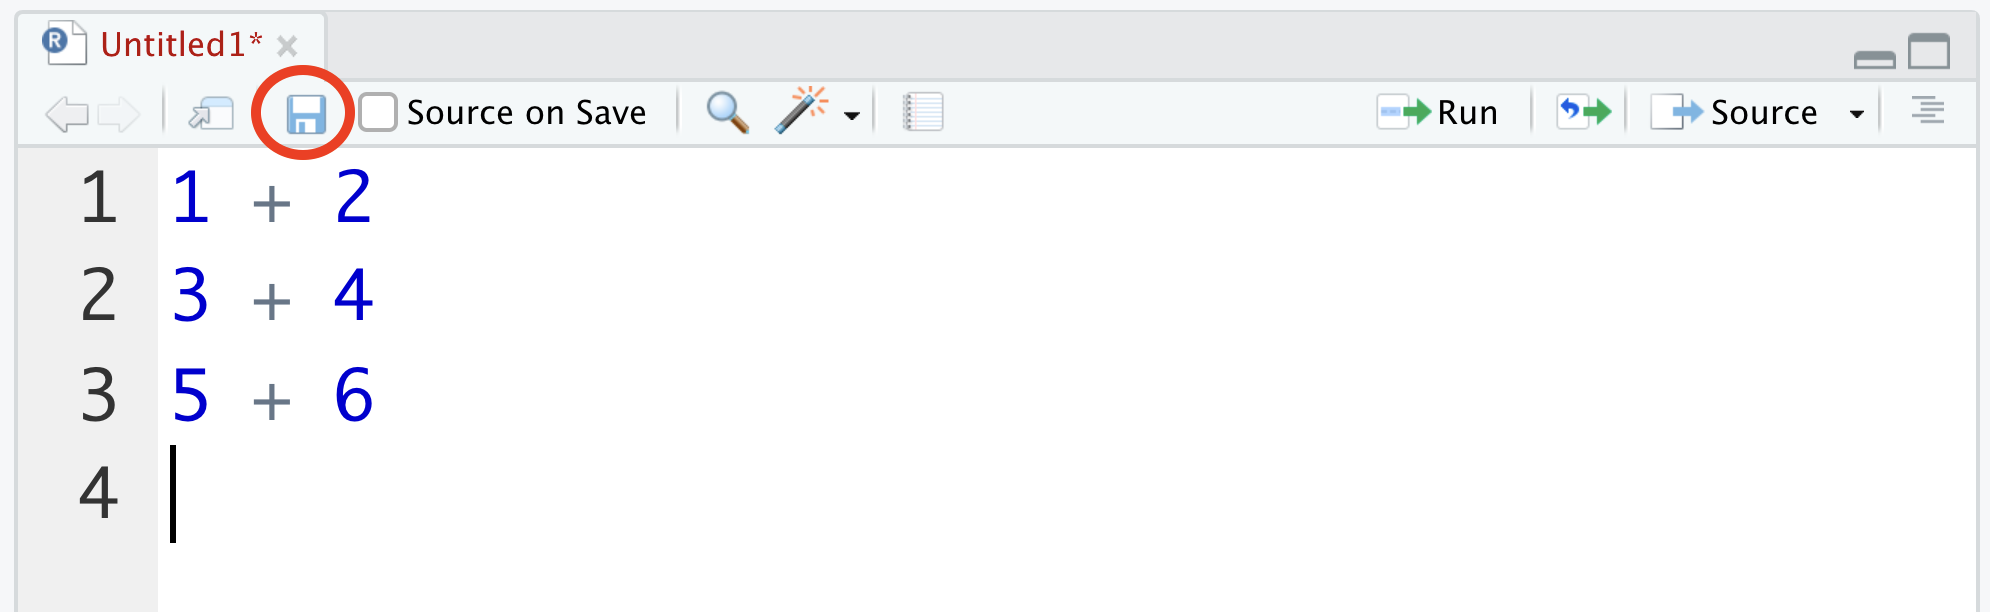
\includegraphics[width=0.7\linewidth]{pics/1save1} 

}

\caption{Save (I)}\label{fig:save1}
\end{figure}

Then you would see a pop-up file dialog box, asking you for a file name and location to save it to. Let's call it lesson1.1 here.

\begin{figure}

{\centering 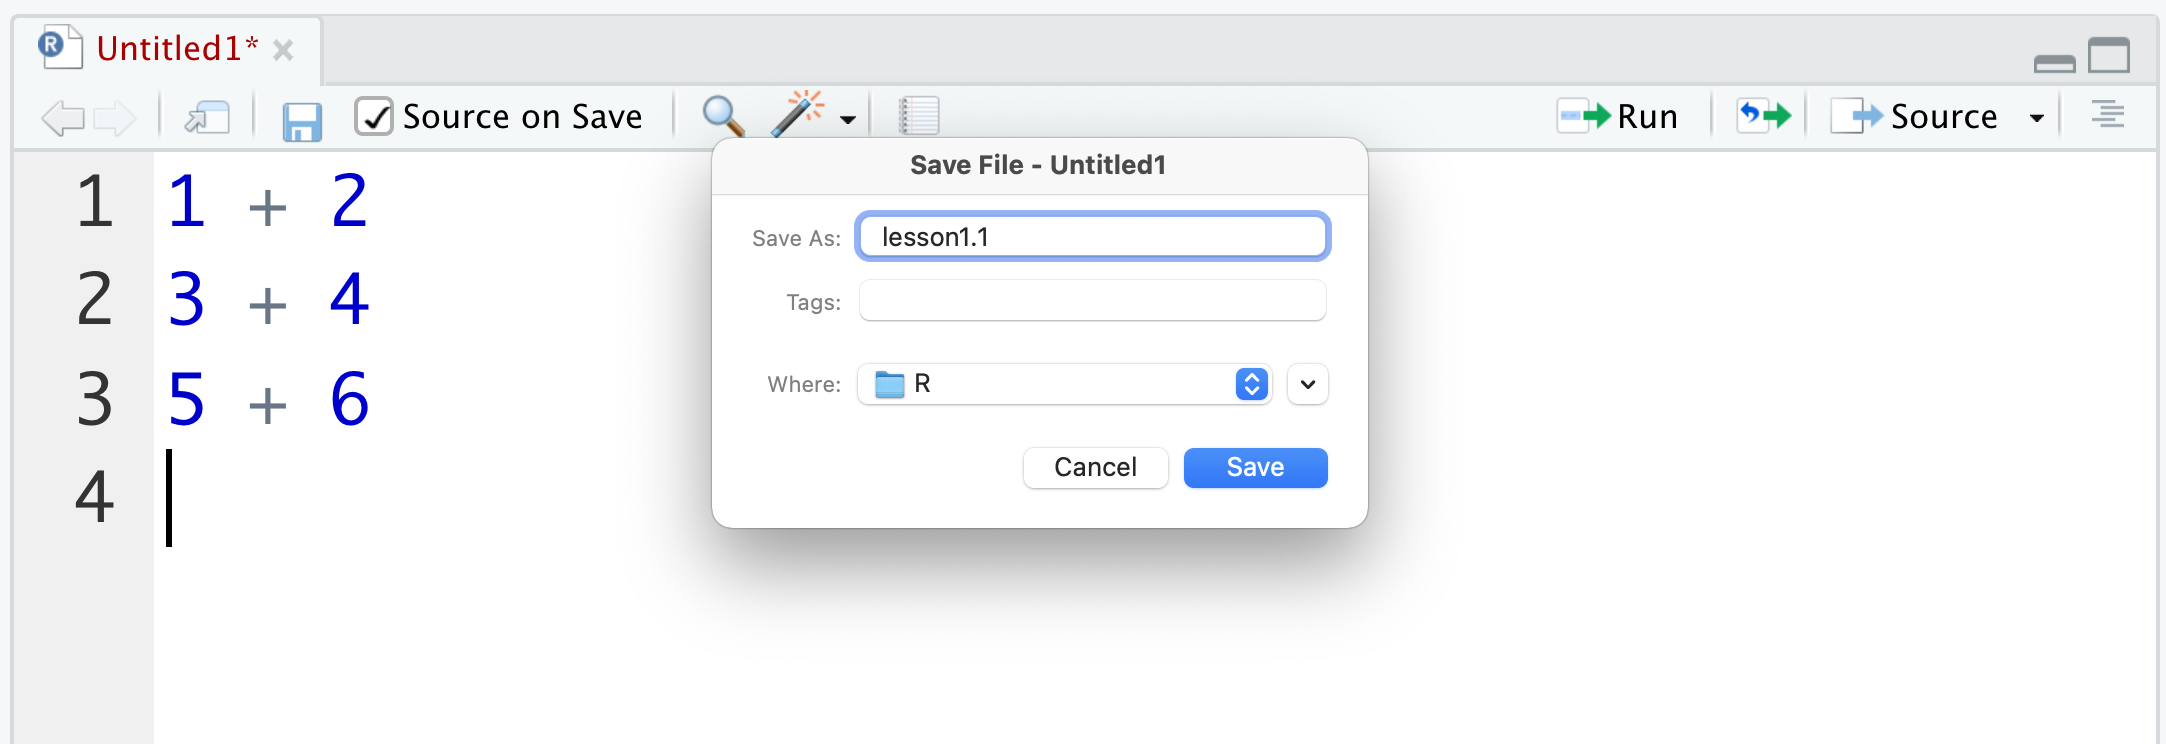
\includegraphics[width=0.7\linewidth]{pics/1save2} 

}

\caption{Save (II)}\label{fig:save2}
\end{figure}

After saving files successfully, you can confirm the name of the R script on the top.

\begin{figure}

{\centering 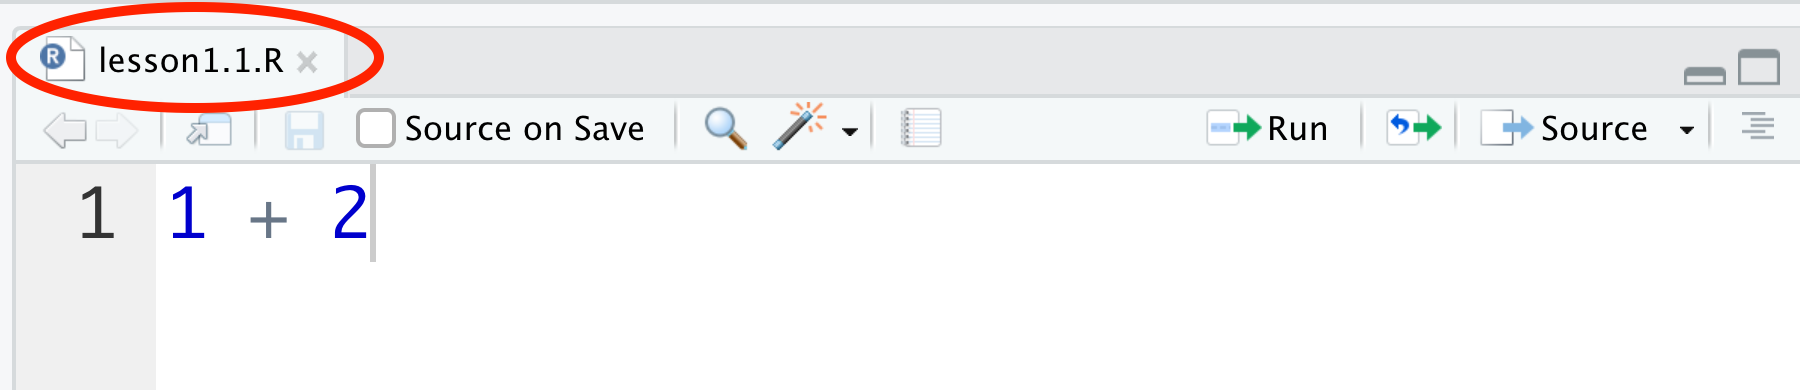
\includegraphics[width=0.7\linewidth]{pics/1save3} 

}

\caption{Save (III)}\label{fig:save3}
\end{figure}

Then if you close this script and open it again, you would directly see the previous three lines of codes without writing them again.

Lastly, if you want to create a new R script, you can click the \texttt{+} button on the menu, then select \emph{R Script}. Note that there are quite a few other options including \emph{R Markdown}, which will be introduced in Chapter \ref{r-markdown}.

\begin{figure}

{\centering 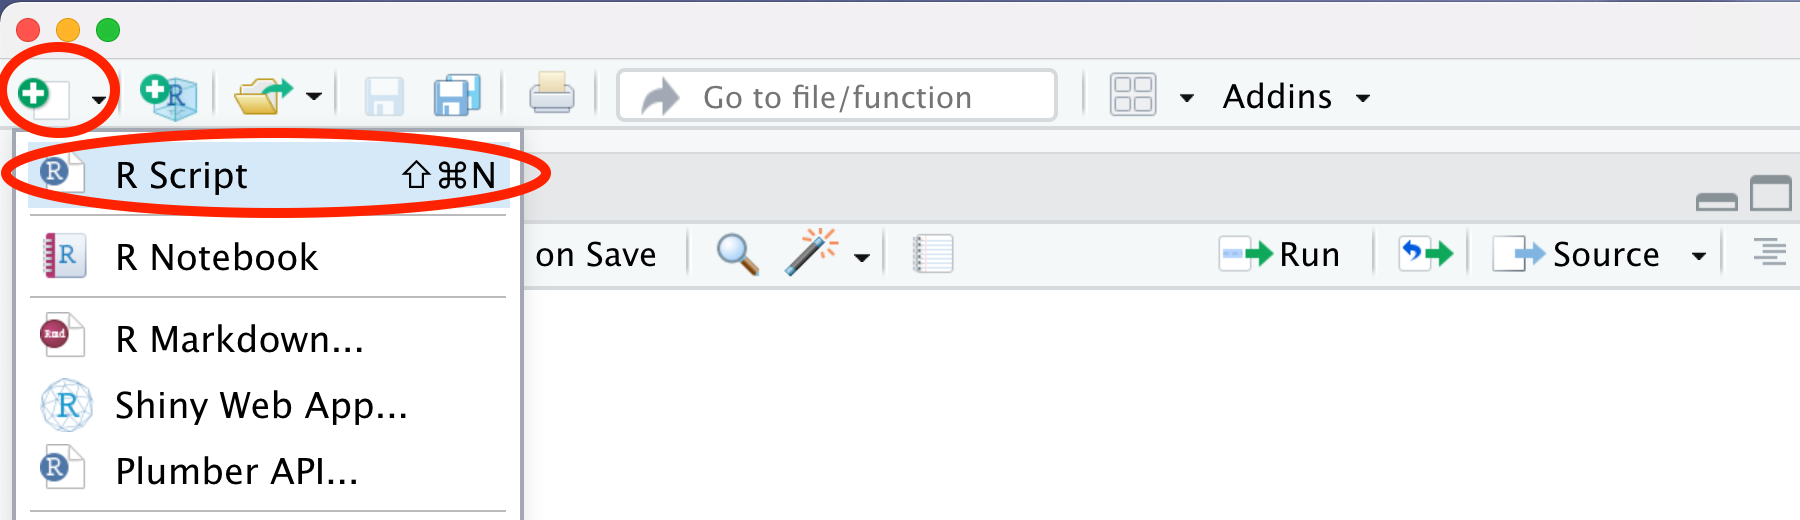
\includegraphics[width=0.7\linewidth]{pics/1new} 

}

\caption{create a new script (I)}\label{fig:new}
\end{figure}

Consequently, you will see a new file created.

\begin{figure}

{\centering 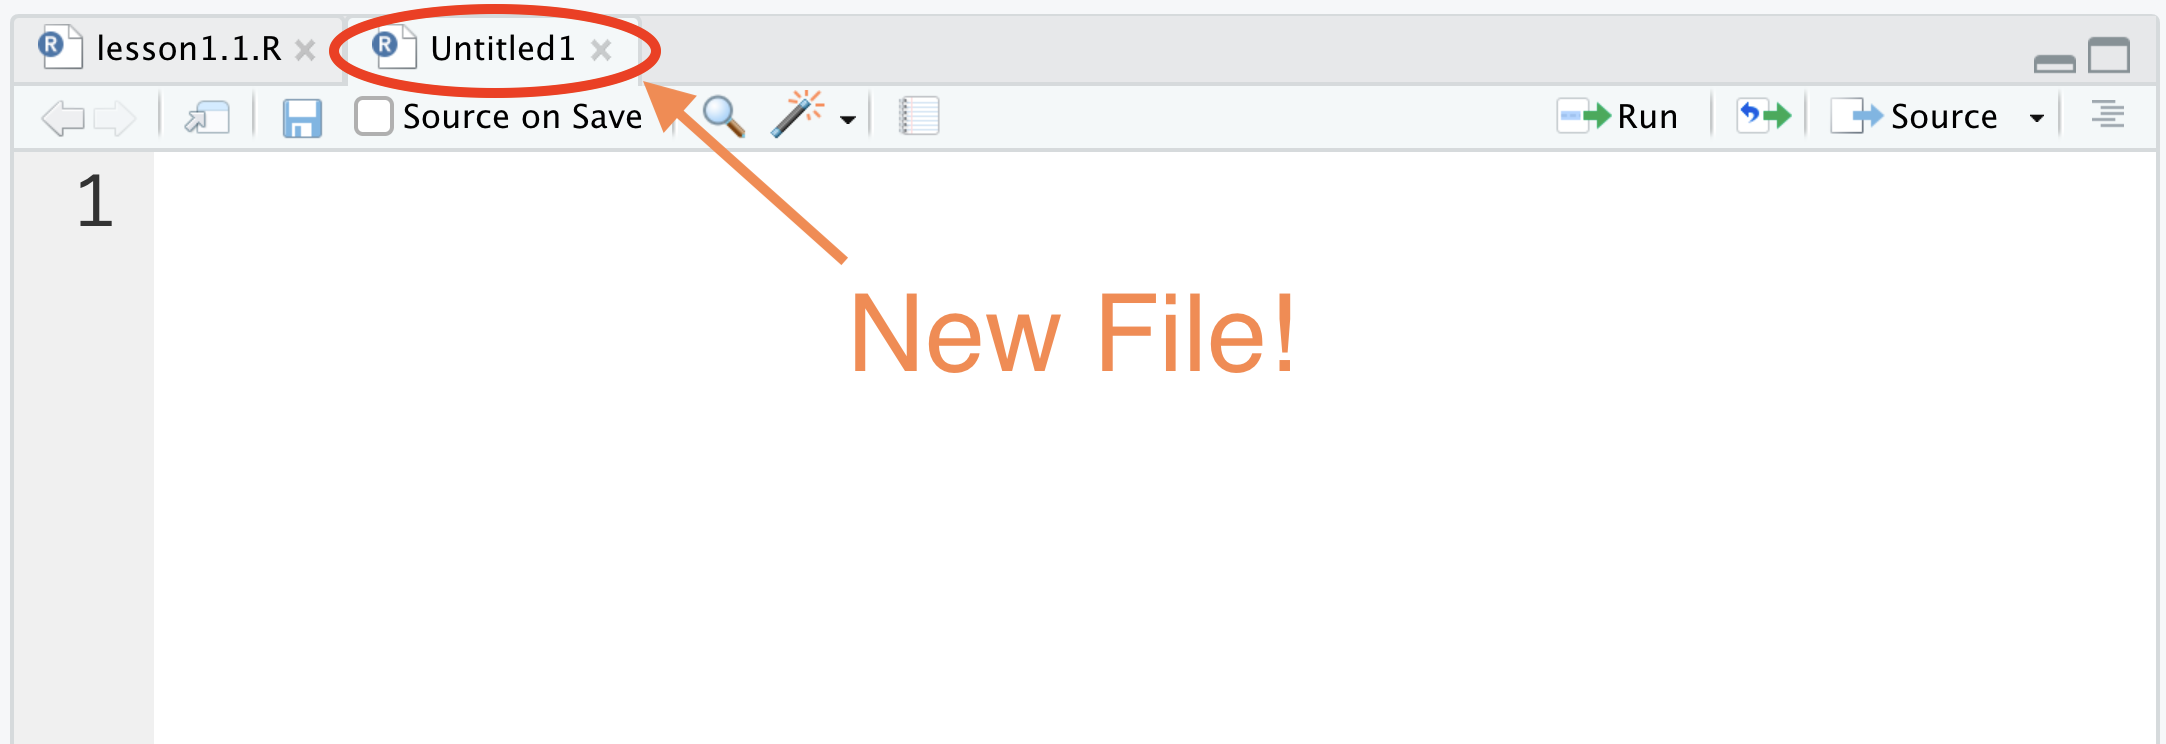
\includegraphics[width=0.7\linewidth]{pics/1new2} 

}

\caption{create a new script (II)}\label{fig:new2}
\end{figure}

\hypertarget{install-and-load-r-packages}{%
\subsection{Install and load R packages}\label{install-and-load-r-packages}}

Now, you have had a basic understanding of RStudio, it is time to meet \textbf{R packages}, which greatly extend the capabilities of base R. There are a large number of publicly available R packages. As of July 2021, there are more than 17K R packages on Comprehensive R Archive Network (CRAN), with many others located in Bioconductor, GitHub, and other repositories.

To install an R package, you need to use a built-in R \textbf{function}, which is \texttt{install.packages()}. A \textbf{function} takes in \textbf{arguments} (inputs) and performs a specific task accordingly. After the function name, we always need to put \textbf{a pair of parentheses} with the arguments inside.

While there are many built-in R functions, R packages usually contain many useful functions as well, and we can also write our own functions, which will be introduced in Chapter \ref{write-code}.

With \texttt{install.packages()}, the argument is the package name with \textbf{a pair of quotation marks} around it. The task it performs is installing the specific package into R. Here, you will install the companion package for this book, named \texttt{r02pro}, a.k.a. \emph{R Zero to Pro}. The \texttt{r02pro} package contains several data sets that will be used throughout the book, and interactive exercises for each subsection.

\begin{Shaded}
\begin{Highlighting}[]
\FunctionTok{install.packages}\NormalTok{(}\StringTok{"r02pro"}\NormalTok{)}
\end{Highlighting}
\end{Shaded}

\begin{infobox}{caution}
If you miss the right parenthesis, R will return a plus in the next line (as shown in Figure \ref{fig:right1}), waiting for more input to complete the command. If this happens, you can either enter the right parenthesis, or press ESC to escape this command. When you see a blinking cursor after the \texttt{\textgreater{}} symbol, you can write new codes again.

\end{infobox}

\begin{figure}

{\centering 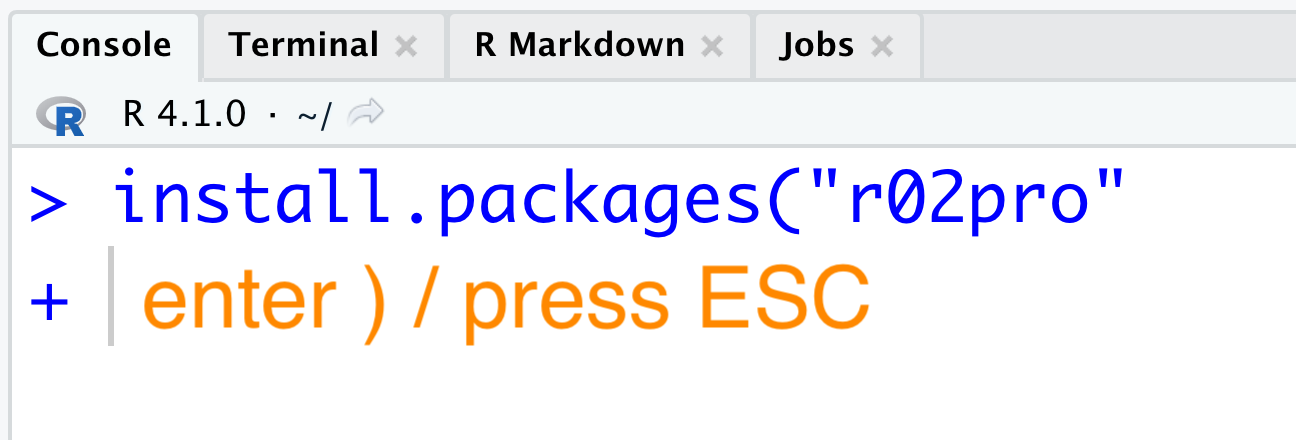
\includegraphics[width=0.7\linewidth]{pics/1right} 

}

\caption{Miss the right parenthesis}\label{fig:right1}
\end{figure}

After a package is installed, you still need to load it into R before using it. To load a package, you can use the \texttt{library()} function with the package name as its argument. Here, quotation marks are not necessary.

\begin{Shaded}
\begin{Highlighting}[]
\FunctionTok{library}\NormalTok{(r02pro)}
\end{Highlighting}
\end{Shaded}

Note that once a package is installed, you \textbf{don't need to} install it again on the same machine. However, when starting a new R session, you would need to load the package again.

\begin{infobox}{caution}

Quotation marks are necessary for installing R packages, but are not necessary for loading packages. When installing packages without quotation marks, you will see an error message, showing \emph{object not found}.

\begin{Shaded}
\begin{Highlighting}[]
\FunctionTok{install.packages}\NormalTok{(r02pro)}
\end{Highlighting}
\end{Shaded}

\end{infobox}

\hypertarget{exercises}{%
\subsection{Exercises}\label{exercises}}

\begin{enumerate}
\def\labelenumi{\arabic{enumi}.}
\tightlist
\item
  Which of the following code used to install packages into R will return an error?
\end{enumerate}

\begin{itemize}
\tightlist
\item
  \texttt{install.packages("r02pro")}
\item
  \texttt{install.packages(r02pro)}
\end{itemize}

\begin{enumerate}
\def\labelenumi{\arabic{enumi}.}
\setcounter{enumi}{1}
\item
  Write the R code to load the package \textbf{r02pro}
\item
  Write the R code to calculate \texttt{2\ +\ 3}.
\end{enumerate}

\hypertarget{Calculator}{%
\section{Use R as a Fancy Calculator}\label{Calculator}}

After learning how to run codes in R, we will introduce how to use R as a fancy calculator.

\hypertarget{add-comments-using}{%
\subsection{Add comments using ``\#''}\label{add-comments-using}}

Before we get started, the first item we will cover is adding comments for codes. In R, you can use the hash character \texttt{\#} at any position of a given line to initiate a comment, and anything after \texttt{\#} will be ignored by R. Let's see an example,

\begin{Shaded}
\begin{Highlighting}[]
\DecValTok{6} \SpecialCharTok{{-}} \DecValTok{1} \SpecialCharTok{/} \DecValTok{2} \CommentTok{\# first calculate 1/2=0.5, then 6{-}0.5=5.5}
\CommentTok{\#\textgreater{} [1] 5.5}
\end{Highlighting}
\end{Shaded}

By running this line of code (either in the console or in the editor!), you will get a value of 5.5, which is the answer of \texttt{6\ -\ 1\ /\ 2}. As demonstrated, R will not run syntax after the hash character \texttt{\#}. Commands and strings after the \texttt{\#} are notations or explanations that can make codes easier to understand. Here, the comment informs you the operation order of previous code: the division is calculated before the subtraction.

In general, adding comments to codes is a very good practice, as it greatly increases readability and make collaboration easier. We will also add necessary comments in our codes to help you learn R.

\hypertarget{basic-calculation}{%
\subsection{Basic calculation}\label{basic-calculation}}

Now let's start to use R as a calculator! In the previous section we introduced operations such as addition, subtraction, multiplication, division, as well as the combination of multiple basic operations. Additionally, you can also calculate the square root, absolute value and the sign of a number.

\begin{tabular}{l|l}
\hline
Operation & Explanation\\
\hline
1 + 2 & addition\\
\hline
1 - 2 & subtraction\\
\hline
2 * 4 & multiplication\\
\hline
2 / 4 & division\\
\hline
6 - 1 / 2 & multiple operations\\
\hline
sqrt(100) & square root\\
\hline
abs(-3) & absolute value\\
\hline
sign(-3) & sign\\
\hline
\end{tabular}

\hypertarget{get-help-in-r}{%
\subsection{Get help in R}\label{get-help-in-r}}

While the first seven operations in the above table look intuitive, you may be wondering, what does the \texttt{sign()} function mean there? Is that a stop sign?

\begin{center}
\includegraphics[width=0.16\linewidth]{pics/1stop} \end{center}

Sometimes, you may have no idea how a particular function works. Fortunately, R provides a detailed documentation for each function.

\textbf{\emph{a. Ask for help}}

First, we will introduce how to ask for help in R, and below are three common ways to seek for more information.

\begin{itemize}
\tightlist
\item
  Use a question mark followed by the function name, e.g.~\texttt{?sign}\\
\item
  Use help function, e.g.~\texttt{help(sign)}
\item
  Use the help window in RStudio, as shown in Figure \ref{fig:help}. The help window is the panel 4 of Figure \ref{fig:four} in Section \ref{Installation}. Then type in the function name in the box to the right of the magnifying glass and press return.
\end{itemize}

\begin{figure}

{\centering 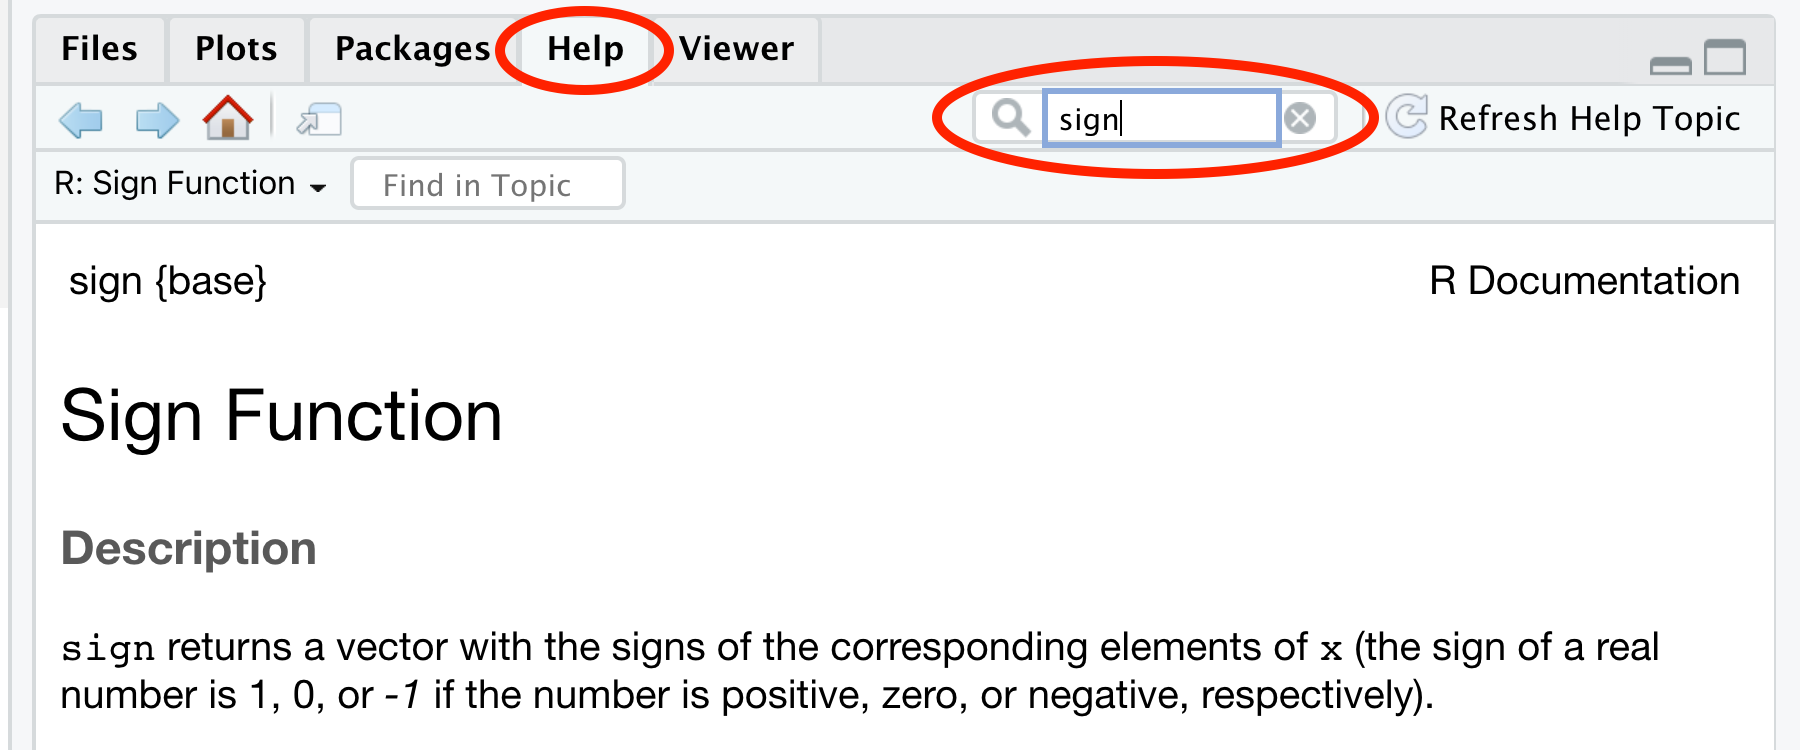
\includegraphics[width=0.7\linewidth]{pics/1help} 

}

\caption{Ask for help}\label{fig:help}
\end{figure}

\textbf{\emph{b. Documentation for functions}}

After using the above operations to ask for help in R, you can get the documentation of the function in the help window. The documentation consists of different parts, let's take the \texttt{sign()} function as an example (Figure \ref{fig:d}),

\begin{figure}

{\centering 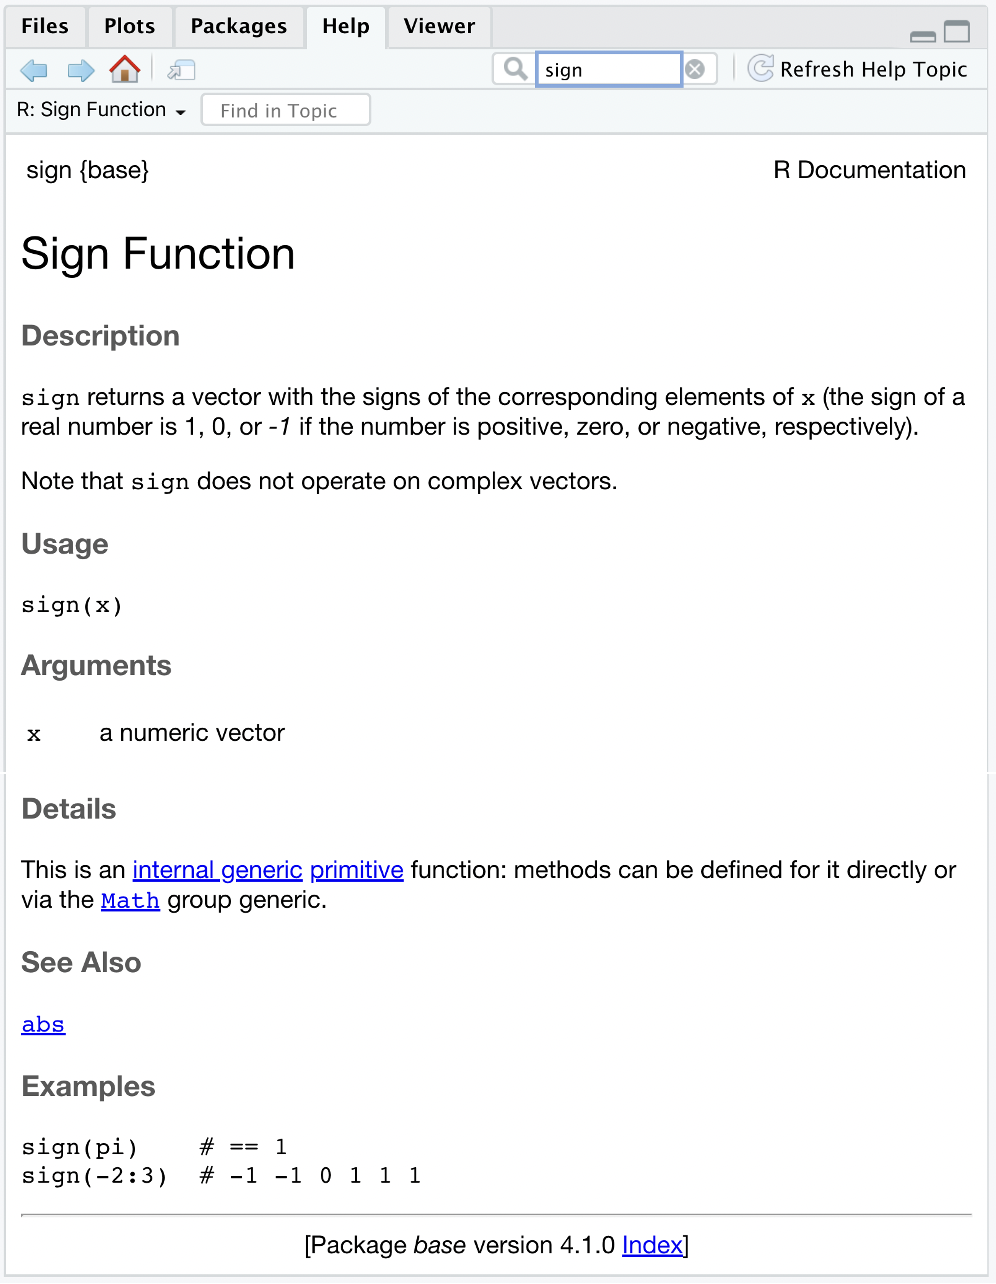
\includegraphics[width=0.7\linewidth]{pics/1d} 

}

\caption{Documentation for function}\label{fig:d}
\end{figure}

This documentation contains the following parts:

\begin{itemize}
\tightlist
\item
  \emph{Description}: A text-format introduction of the function of interest. The introduction describes the function's mechanism, the acceptable input and output types, and some notes of the function.
\item
  \emph{Usage}: The way the function looks like.
\item
  \emph{Arguments}: A detailed description of the input.
\item
  \emph{Details}: A detailed description of the function, including the background, some complicated usage, and special cases of the function.
\item
  \emph{See Also}: Some functions related or similar to this function.
\item
  \emph{Examples}: Sample codes and their corresponding answers. You can simply copy codes in the \emph{Examples} part and run them in the editor or in the console. Note that all words after \texttt{\#} are comments and will be ignored by R.
\end{itemize}

Here, from the documentation of the \texttt{sign()} function, you will know that the \texttt{sign()} function can return the signs of numbers, which means it will return 0 for zero, return 1 for positive numbers, and return -1 for negative numbers.

The documentation of different functions can contain different parts, we will give you the introduction of other functions in the following sections.

\hypertarget{approximation}{%
\subsection{Approximation}\label{approximation}}

Next, let's move on to the approximation in R. When computing \texttt{7\ /\ 3}, the answer is not a whole number as 7 is not divisible by 3. Approximation will come in handy under such circumstances. Let's take \texttt{7\ /\ 3} as the example.

\textbf{\emph{a. Get the integer part and the remainder}}

\begin{tabular}{l|l}
\hline
Code & Name\\
\hline
7\%/\%3 & integer division\\
\hline
7\%\%3 & modulus\\
\hline
\end{tabular}

We all know that 7 = 3 * \textbf{2} + \textbf{1}. So the \emph{integer division} will pick up the integer part, which is 2 here; and the \emph{modulus} will get the remainder, which is 1.

\textbf{\emph{b. Get the nearby integer}}

\begin{Shaded}
\begin{Highlighting}[]
\FunctionTok{floor}\NormalTok{(}\DecValTok{7} \SpecialCharTok{/} \DecValTok{3}\NormalTok{)   }
\CommentTok{\#\textgreater{} [1] 2}
\FunctionTok{ceiling}\NormalTok{(}\DecValTok{7} \SpecialCharTok{/} \DecValTok{3}\NormalTok{) }
\CommentTok{\#\textgreater{} [1] 3}
\end{Highlighting}
\end{Shaded}

Since \textbf{2} \textless= 7/3 \textless= \textbf{3}, you can use the \texttt{floor} function to find the \emph{largest integer} \textless= 7/3, which is 2; and the \texttt{ceiling} function gives the \emph{smallest integer} \textgreater= 7/3, which is 3.

\textbf{\emph{c.~Round to the nearest number}}

\begin{Shaded}
\begin{Highlighting}[]
\FunctionTok{round}\NormalTok{(}\DecValTok{7} \SpecialCharTok{/} \DecValTok{3}\NormalTok{)   }
\CommentTok{\#\textgreater{} [1] 2}
\FunctionTok{round}\NormalTok{(}\DecValTok{7} \SpecialCharTok{/} \DecValTok{3}\NormalTok{, }\AttributeTok{digits =} \DecValTok{3}\NormalTok{)}
\CommentTok{\#\textgreater{} [1] 2.333}
\end{Highlighting}
\end{Shaded}

The \texttt{round()} function follows the \textbf{rounding principle}. By default, you will get the nearest integer to \texttt{7\ /\ 3}, which is \texttt{2}. If you want to control the approximation accuracy, you can add a \texttt{digits} argument to specify how many digits you want after the decimal point. Here you will get \texttt{2.333} after adding \texttt{digits\ =\ 3}.

\hypertarget{power-logarithm}{%
\subsection{Power \& logarithm}\label{power-logarithm}}

You can also use R to do \emph{power} and \emph{logarithmic} operations.

Generally, you can use \texttt{\^{}} to do power operations. For example, \texttt{10\^{}5} will give us 10 to the power of 5. Here, 10 is the \emph{base} value, and 5 is the \emph{exponent}. The result is 100000, but it is shown as \texttt{1e+05} in R. That's because R uses the so-called \emph{scientific notation}.

\begin{infobox}{caution}
\textbf{scientific notation}: a common way to express numbers which are too large or too small to be conveniently written in decimal form. Generally, it expresses numbers in forms of \(m \times 10^n\) and R uses the \textbf{e notation}. Note that the \textbf{e notation} has nothing to do with the natural number \(e\). Let's see some examples,
\begin{align}
1 \times 10^5 &= \mbox{1e+05}\\
2 \times 10^4 &= \mbox{2e+04}\\
1.2 \times 10^{-3} &= \mbox{1.2e-03}
\end{align}

\end{infobox}

In mathematics, the \emph{logarithmic operations} are inverse to the power operations. If \textbf{\(b^y = x\)} and you only know \emph{\(b\)} and \emph{\(x\)}, you can do logarithmic operations to solve \emph{\(y\)} using the general form \textbf{\(y = \log(x, b)\)}, which is called the logarithm of \(x\) with base \(b\).

In R, logarithm functions with base value of 10, 2, or the natural number \(e\) have shortcuts \texttt{log10()}, \texttt{log2()}, and \texttt{log()}, respectively. Let's see an example of \texttt{log10()}, the logarithm function with base \emph{10}. Here, we have added a comment to help you have a better understanding of \texttt{log10()}.

\begin{Shaded}
\begin{Highlighting}[]
\DecValTok{10}\SpecialCharTok{\^{}}\DecValTok{6} 
\CommentTok{\#\textgreater{} [1] 1e+06}
\FunctionTok{log10}\NormalTok{(}\FloatTok{1e6}\NormalTok{) }\CommentTok{\#log10(x) = log(x, 10)}
\CommentTok{\#\textgreater{} [1] 6}
\end{Highlighting}
\end{Shaded}

Next, let's see \texttt{log2()}, the logarithm function with base \emph{2}. There is also a comment for \texttt{log2()} here.

\begin{Shaded}
\begin{Highlighting}[]
\DecValTok{2}\SpecialCharTok{\^{}}\DecValTok{10}
\CommentTok{\#\textgreater{} [1] 1024}
\FunctionTok{log2}\NormalTok{(}\DecValTok{1024}\NormalTok{)  }\CommentTok{\#log2(x) = log(x, 2)}
\CommentTok{\#\textgreater{} [1] 10}
\end{Highlighting}
\end{Shaded}

Before moving on to the natural logarithm, note that the natural number \(e\) needs to be written as \texttt{exp(1)} in R. When you want to do power operations on \(e\), you can simply change the argument in the function \texttt{exp()}. For example, \texttt{exp(3)} is \(e\) to the power of 3. Here, \texttt{log()} without specifying the \texttt{base} argument represents the logarithm function with base \(e\). You can see the general form of \texttt{log()} in the comment.

\begin{Shaded}
\begin{Highlighting}[]
\FunctionTok{exp}\NormalTok{(}\DecValTok{1}\NormalTok{)      }
\CommentTok{\#\textgreater{} [1] 2.718282}
\FunctionTok{exp}\NormalTok{(}\DecValTok{3}\NormalTok{)}
\CommentTok{\#\textgreater{} [1] 20.08554}
\FunctionTok{log}\NormalTok{(}\FunctionTok{exp}\NormalTok{(}\DecValTok{3}\NormalTok{))  }\CommentTok{\#log(x) = log(x, exp(1))}
\CommentTok{\#\textgreater{} [1] 3}
\end{Highlighting}
\end{Shaded}

\hypertarget{trigonometric-function}{%
\subsection{Trigonometric function}\label{trigonometric-function}}

R also provides the common trigonometric functions.

\begin{Shaded}
\begin{Highlighting}[]
\FunctionTok{cos}\NormalTok{(pi)}
\CommentTok{\#\textgreater{} [1] {-}1}
\FunctionTok{acos}\NormalTok{(}\SpecialCharTok{{-}}\DecValTok{1}\NormalTok{)}
\CommentTok{\#\textgreater{} [1] 3.141593}
\end{Highlighting}
\end{Shaded}

Here, \texttt{acos()} is the inverse function of \texttt{cos()}. If we set \(cos(a) = b\), then we will get \(acos(b) = a\).

\begin{Shaded}
\begin{Highlighting}[]
\FunctionTok{sin}\NormalTok{(pi}\SpecialCharTok{/}\DecValTok{2}\NormalTok{)}
\CommentTok{\#\textgreater{} [1] 1}
\FunctionTok{asin}\NormalTok{(}\DecValTok{1}\NormalTok{)}
\CommentTok{\#\textgreater{} [1] 1.570796}
\end{Highlighting}
\end{Shaded}

Similarly, \texttt{asin()} is the inverse function of \texttt{sin()}. If we set \(sin(a) = b\), then we will get \(asin(b) = a\).

\begin{Shaded}
\begin{Highlighting}[]
\FunctionTok{tan}\NormalTok{(pi}\SpecialCharTok{/}\DecValTok{4}\NormalTok{)}
\CommentTok{\#\textgreater{} [1] 1}
\FunctionTok{atan}\NormalTok{(}\DecValTok{1}\NormalTok{)}
\CommentTok{\#\textgreater{} [1] 0.7853982}
\end{Highlighting}
\end{Shaded}

Also, \texttt{atan()} is the inverse function of \texttt{tan()}. If we set \(tan(a) = b\), then we will get \(atan(b) = a\).

\hypertarget{exercises-1}{%
\subsection{Exercises}\label{exercises-1}}

\begin{enumerate}
\def\labelenumi{\arabic{enumi}.}
\item
  Write R code to compute \(\sqrt{5 \times 5}\).
\item
  Write R code to get help on the function \texttt{floor}.
\item
  Write R code to compute the square of \(\pi\) and round it to 4 digits after the decimal point.
\item
  Write R code to compute the logarithm of 1 billion with base 1000.
\item
  Write R code to verify \(sin^2(x) + cos^2(x) = 1\), for \(x = 724\).
\end{enumerate}

\hypertarget{Object-Assignment}{%
\section{Object Assignment}\label{Object-Assignment}}

In the last section, you have seen the power of R as a fancy calculator. However, in order to do more complicated and interesting tasks, it is super helpful to store intermediate results for future use.

Let's take a look at a concrete example. Say if you want to do the following three calculations, all involving \texttt{exp(3)\ /\ log(20,3)\ *\ 7}.

\begin{Shaded}
\begin{Highlighting}[]
\NormalTok{(}\FunctionTok{exp}\NormalTok{(}\DecValTok{3}\NormalTok{) }\SpecialCharTok{/} \FunctionTok{log}\NormalTok{(}\DecValTok{20}\NormalTok{,}\DecValTok{3}\NormalTok{) }\SpecialCharTok{*} \DecValTok{7}\NormalTok{) }\SpecialCharTok{+} \DecValTok{3} \CommentTok{\#addition}
\NormalTok{(}\FunctionTok{exp}\NormalTok{(}\DecValTok{3}\NormalTok{) }\SpecialCharTok{/} \FunctionTok{log}\NormalTok{(}\DecValTok{20}\NormalTok{,}\DecValTok{3}\NormalTok{) }\SpecialCharTok{*} \DecValTok{7}\NormalTok{) }\SpecialCharTok{{-}} \DecValTok{3} \CommentTok{\#subtraction}
\NormalTok{(}\FunctionTok{exp}\NormalTok{(}\DecValTok{3}\NormalTok{) }\SpecialCharTok{/} \FunctionTok{log}\NormalTok{(}\DecValTok{20}\NormalTok{,}\DecValTok{3}\NormalTok{) }\SpecialCharTok{*} \DecValTok{7}\NormalTok{) }\SpecialCharTok{/} \DecValTok{3} \CommentTok{\#division}
\end{Highlighting}
\end{Shaded}

Using R as a fancy calculator (Section \ref{Calculator}), you need to type the expression \texttt{exp(3)\ /\ log(20,3)\ *\ 7} three times, which is a bit cumbersome. In this section, you will learn how to do \textbf{object assignment}, which can avoid the need for typing the same expression more than once.

\hypertarget{what-is-an-r-object}{%
\subsection{What is an R Object?}\label{what-is-an-r-object}}

Before we get into the details, let's first introduce \textbf{object}, which is perhaps the most fundamental thing in R. In principle, \textbf{everything that exists in R is an object}. For example, the number \texttt{5} is an object, the expression \texttt{1\ +\ 2} is an object, and the expression \texttt{exp(3)\ /\ log(20,3)\ *\ 7} is also an object.

If you run \texttt{5}, you will get one element of value 5 from the output. Similarly, if you run \texttt{1\ +\ 2}, you will get one element of value 3 from the output. You can try to run \texttt{exp(3)\ /\ log(20,3)\ *\ 7} by yourself. In these three examples, you can see that there is only one \textbf{element} in each object.

However, an object can contain more than one elements, and each element has its own \textbf{value}, which is possibly different from that of another element. Naturally, different objects can contain different values.

\hypertarget{assignment}{%
\subsection{\texorpdfstring{Assignment Operation with \texttt{\textless{}-}}{Assignment Operation with \textless-}}\label{assignment}}

With the importance of objects in mind, let's learn how to do \textbf{object assignments} in R. To do object assignments, you need to assign \textbf{value(s)} to a \textbf{name} via the \textbf{assignment operator}, which will create a new object with the name you specified. Once the object assignment operation is done, you can simply use the name in subsequent calculations without redundancy. Let's start with a simple example,

\begin{Shaded}
\begin{Highlighting}[]
\NormalTok{x\_num }\OtherTok{\textless{}{-}} \DecValTok{5}
\end{Highlighting}
\end{Shaded}

The assignment operation has three components. From left to right,

\begin{itemize}
\tightlist
\item
  the first component \texttt{x\_num} is the \textbf{object name} of a new object, which has certain naming rules that will be discussed shortly in Section \ref{Naming}.
\item
  The second component is the \textbf{assignment operator} \texttt{\textless{}-}, which is a combination of the less than sign \texttt{\textless{}} immediately followed by the minus sign \texttt{-}, with \textbf{no space} in between.
\item
  The final component is the object name's assigned \textbf{value(s)}, which is 5 here.
\end{itemize}

\begin{infobox}{caution}
There is no space between \texttt{\textless{}} and \texttt{-} in the assignment operator \texttt{\textless{}-}. Note that although \texttt{=} may also appear to be working as the assignment operator, it is not recommended as \texttt{=} is usually reserved for specifying the value(s) of arguments in a function call, which will be introduced in Section \ref{vector-patterns}.

\end{infobox}

After running the code above, you will see no output in the console, unlike the situation when we ran \texttt{1\ +\ 2} which gives us the answer \texttt{3} (as shown in Figure \ref{fig:noa}). You may be wondering, did we successfully make our first assignment operation?

\begin{figure}

{\centering 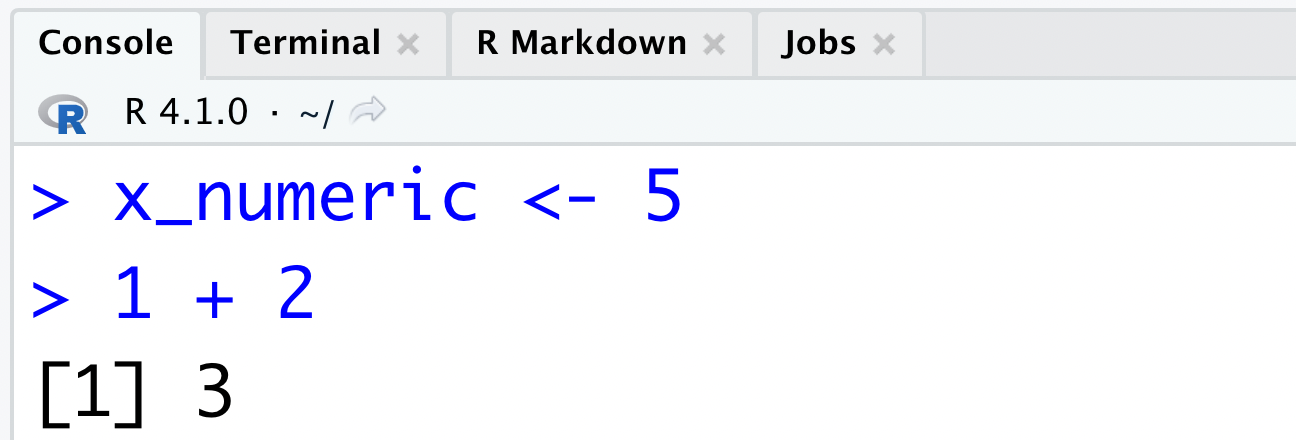
\includegraphics[width=0.7\linewidth]{pics/2noa} 

}

\caption{No output}\label{fig:noa}
\end{figure}

To verify it, you can run the code with just the object name to check its value. (For all named objects, you can get their value(s) by running codes with just their names.)

\begin{Shaded}
\begin{Highlighting}[]
\NormalTok{x\_num}
\CommentTok{\#\textgreater{} [1] 5}
\end{Highlighting}
\end{Shaded}

Great! The output is 5, indicating that you have successfully assigned the value 5 to the name x\_num, and you have created a new object \texttt{x\_num}. You can use \texttt{x\_num} instead of \texttt{5} to do the subsequent calculations because \texttt{x\_num} and \texttt{5} have the same value.

Note that R object names are \textbf{case-sensitive}. For example, you have defined \texttt{x\_num}, but if you type \texttt{X\_num}, the console will return an error message as follow.

\begin{Shaded}
\begin{Highlighting}[]
\NormalTok{X\_num}
\CommentTok{\#\textgreater{} Error in eval(expr, envir, enclos): object \textquotesingle{}X\_num\textquotesingle{} not found}
\end{Highlighting}
\end{Shaded}

In addition, you can assign \textbf{value(s)} of an expression to a name. Let's try to simplify the three expressions we showed at the beginning of this section. It is easy to observe that the three expressions share a common term \texttt{exp(3)\ /\ log(20,3)\ *\ 7}. Let's assign the common term to a name.

\begin{Shaded}
\begin{Highlighting}[]
\NormalTok{y\_num }\OtherTok{\textless{}{-}} \FunctionTok{exp}\NormalTok{(}\DecValTok{3}\NormalTok{) }\SpecialCharTok{/} \FunctionTok{log}\NormalTok{(}\DecValTok{20}\NormalTok{,}\DecValTok{3}\NormalTok{) }\SpecialCharTok{*} \DecValTok{7}
\NormalTok{y\_num}
\CommentTok{\#\textgreater{} [1] 51.56119}
\end{Highlighting}
\end{Shaded}

Now you have successfully created an object \texttt{y\_num} with value 51.561191. Using the named object \texttt{y\_num}, you can simplify the three calculations as follows.

\begin{Shaded}
\begin{Highlighting}[]
\NormalTok{y\_num }\SpecialCharTok{+} \DecValTok{3}
\NormalTok{y\_num }\SpecialCharTok{{-}} \DecValTok{3}
\NormalTok{y\_num }\SpecialCharTok{/} \DecValTok{3}
\end{Highlighting}
\end{Shaded}

\begin{infobox}{caution}
Note that in the object assignment process, it is not the expression itself but rather the value(s) of the expression, that is assigned to a name. So you will not get the expression \texttt{exp(3)\ /\ log(20,3)\ *\ 7} by running \texttt{y\_num}.

\end{infobox}

You can also try the following examples by yourself.

\begin{Shaded}
\begin{Highlighting}[]
\NormalTok{z\_num1 }\OtherTok{\textless{}{-}} \FunctionTok{floor}\NormalTok{(}\DecValTok{7} \SpecialCharTok{/} \DecValTok{3}\NormalTok{) }
\NormalTok{z\_num1}
\NormalTok{z\_num2 }\OtherTok{\textless{}{-}} \DecValTok{7}\SpecialCharTok{\%/\%}\DecValTok{3}
\NormalTok{z\_num2}
\end{Highlighting}
\end{Shaded}

Clearly, using the object assignment, you can greatly simplify the code and avoid redundancy.

\hypertarget{Naming}{%
\subsection{Object naming rule}\label{Naming}}

As you now see, the assignment operation in R is very straightforward. In general, R is very flexible in the name you can give to an object. However, there are three important rules you need to follow.

\textbf{\emph{a. Must start with a letter or . (period)}}

In addition, if starting with period, the second character can't be a number.

\textbf{\emph{b. Can only contain letters, numbers, \texttt{\_} (underscore), and \texttt{.} (period)}}

One recommended naming style is to use lowercase letters and numbers, and use underscore to separate words within a name. So you can use relatively longer names that is more readable. For example, \texttt{this\_is\_name\_6} and \texttt{super\_rich\_88} are great names.

\textbf{\emph{c.~Can not use special keywords as names.}}

For example, \texttt{TRUE\ \textless{}-\ 12} is not permitted as \texttt{TRUE} is a special keyword in R. You can see from the following that this assignment operation leads to an error message.

\begin{Shaded}
\begin{Highlighting}[]
\ConstantTok{TRUE} \OtherTok{\textless{}{-}} \DecValTok{12}
\CommentTok{\#\textgreater{} Error in TRUE \textless{}{-} 12: invalid (do\_set) left{-}hand side to assignment}
\end{Highlighting}
\end{Shaded}

Some commonly used reserved keywords that cannot be used as names are listed as below.

\begin{tabular}{l|l}
\hline
TRUE & else\\
\hline
FALSE & for\\
\hline
NA & while\\
\hline
Inf & break\\
\hline
NaN & next\\
\hline
function & repeat\\
\hline
if & return\\
\hline
\end{tabular}

To get a complete list of reserved words, you can run the following code.

\begin{Shaded}
\begin{Highlighting}[]
\NormalTok{?Reserved}
\end{Highlighting}
\end{Shaded}

\hypertarget{review-objects-in-environment}{%
\subsection{Review objects in environment}\label{review-objects-in-environment}}

At this point, we've introduced the rules of creating objects in R. Now, you can also confirm the success of object assignments by inspecting the \textbf{Environment}, located in the top right panel (\textbf{panel3 in Figure \ref{fig:four} in Section \ref{Installation}}).

If you exercised previous examples, you can find the newly assigned objects \texttt{x\_num} and \texttt{y\_num} (possibly also \texttt{z\_num1} and \texttt{z\_num2}) in your \emph{Environment} Viewer. You may also notice that the name \texttt{TRUE}, which we tried but failed to assign the value 12 to, doesn't appear in the \emph{Environment} (as shown in Figure \ref{fig:en}). You can check all the \textbf{named objects} and their values in this area. It is helpful to monitor the environment from time to time to make sure everything looks fine. Notice that objects without names will \emph{not} be shown in the environment.

\begin{figure}

{\centering 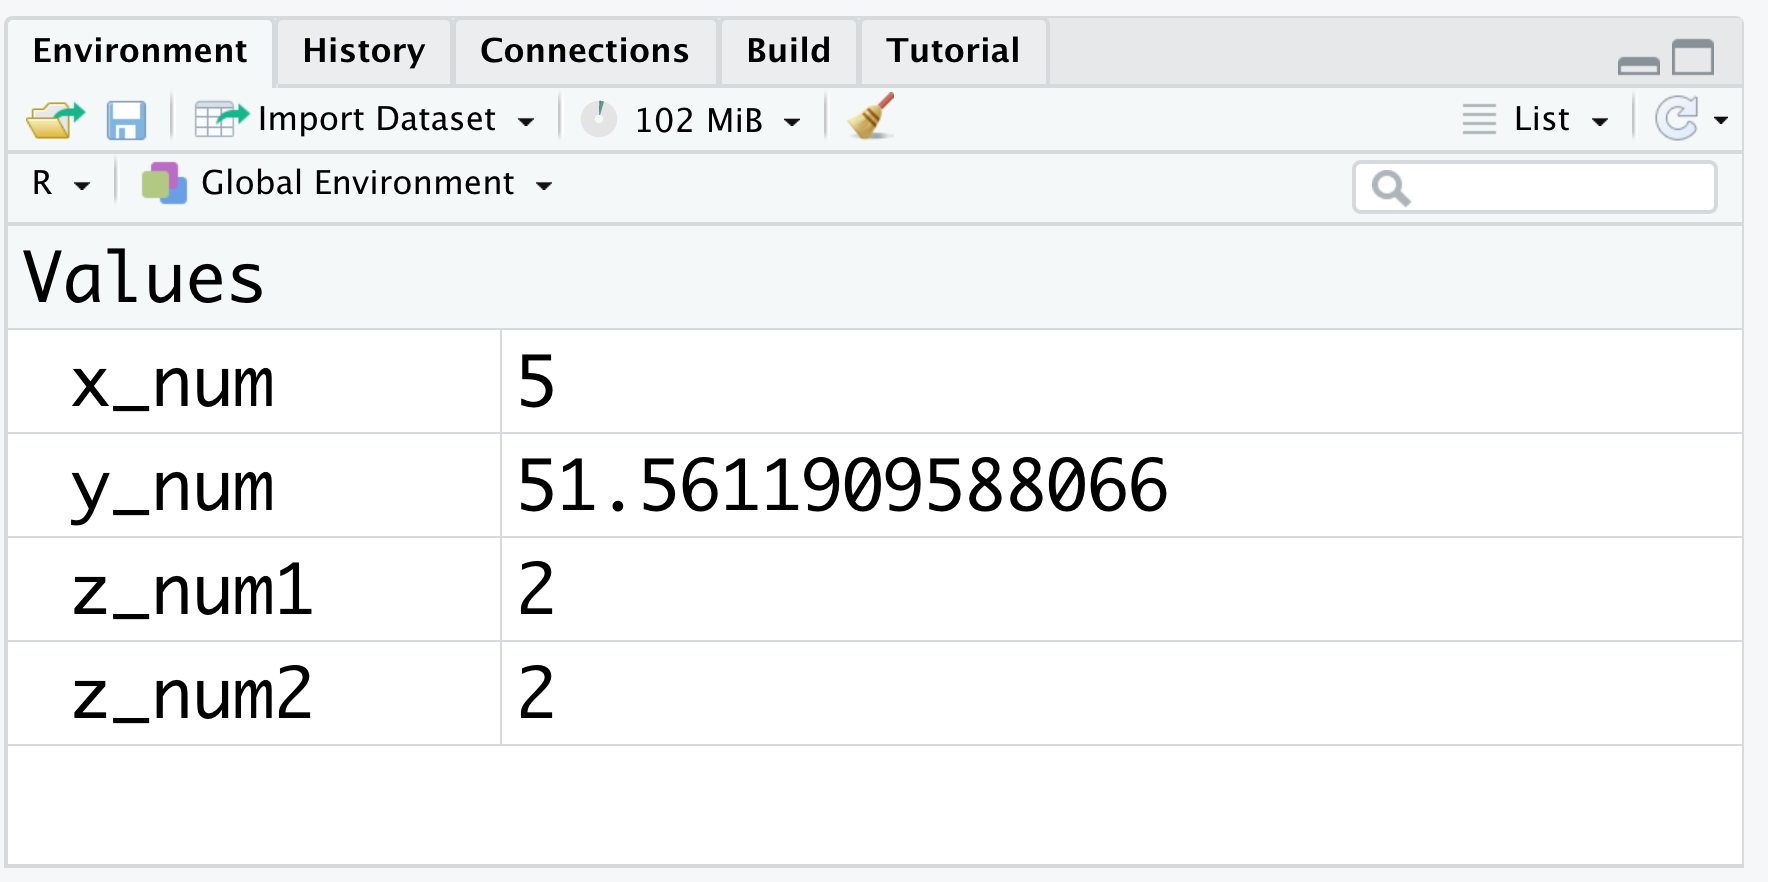
\includegraphics[width=0.7\linewidth]{pics/1en} 

}

\caption{The environment}\label{fig:en}
\end{figure}

You can also see the list of all the named objects using the built-in R function \texttt{ls()}.

\begin{Shaded}
\begin{Highlighting}[]
\FunctionTok{ls}\NormalTok{()}
\CommentTok{\#\textgreater{} [1] "key\_mat" "Keys"    "x\_num"   "y\_num"}
\end{Highlighting}
\end{Shaded}

All the objects shown in the environment or on the list are stored in the memory, so they are available for us in subsequent codes. It is a good habit to do object assignments if you want to retrieve their values at a later time.

\hypertarget{object-types}{%
\subsection{Object types}\label{object-types}}

So far in this section, you have learned how to do object assignments. The values you assigned are all numbers, i.e.~of numeric type. Actually, an object may contain more than one values. Also, an object may contain values other than the numeric type, such like character and logical ones. Depending on the \textbf{composition of values}, the object belongs to one particular type.

\begin{tabular}{l|l}
\hline
Type & Section\\
\hline
Atomic Vector & \textbackslash{}@ref(r-objects)\\
\hline
Matrix & \textbackslash{}@ref(matrix)\\
\hline
Array & \textbackslash{}@ref(array)\\
\hline
Data Frame & \textbackslash{}@ref(dataframe)\\
\hline
Tibble & \textbackslash{}@ref(tibble)\\
\hline
List & \textbackslash{}@ref(list)\\
\hline
\end{tabular}

We will focus on atomic vectors in Chapter \ref{r-objects} and discuss other object types in Chapter \ref{r-objects-other-types}.

While some of the object types look more intuitive than others, you have nothing to worry about since we have the next two chapters devoted to the details of R objects. Objects are the building blocks of R programming and it will be time well spent mastering every object type.

\hypertarget{exercises-2}{%
\subsection{Exercises}\label{exercises-2}}

\begin{enumerate}
\def\labelenumi{\arabic{enumi}.}
\item
  Write the R code to assign the value 20 to the name \texttt{num\_1}.
\item
  Which of the following is a valid object name in R?
\end{enumerate}

\begin{itemize}
\tightlist
\item
  \texttt{2.True}
\item
  \texttt{else}
\item
  \texttt{I\_am\_not\_a\_valid\_name}
\item
  \texttt{I\_am\_a\_Pretty\#\_name}
\end{itemize}

\begin{enumerate}
\def\labelenumi{\arabic{enumi}.}
\setcounter{enumi}{2}
\tightlist
\item
  Write the R code to get the list of all objects in the environment.
\end{enumerate}

\hypertarget{head}{%
\chapter{\textless\textless\textless\textless\textless\textless\textless{} HEAD}\label{head}}

\begin{quote}
\begin{quote}
\begin{quote}
\begin{quote}
\begin{quote}
\begin{quote}
\begin{quote}
e5b4e15619ce4762dabe335c7edeccecb8a5b818
\end{quote}
\end{quote}
\end{quote}
\end{quote}
\end{quote}
\end{quote}
\end{quote}

\hypertarget{r-objects}{%
\chapter{R Objects (I): Atomic Vectors}\label{r-objects}}

In this chapter, we focus on the most fundamental R object type: \textbf{atomic vectors}. We will introduce different types of atomic vectors, creating vectors with patterns, applying different functions and operations on vectors, comparing and extracting vectors. We will also discuss data and times, factors, and how R represents unexpected results.

\hypertarget{intro-num-vector}{%
\section{Introduction to Numeric Vectors}\label{intro-num-vector}}

We will start off this chapter by learning \textbf{numeric vectors}. Numeric vectors are perhaps the most commonly used member of the \textbf{atomic vector} family, where all elements are of the same type.

\hypertarget{create-numeric-vector}{%
\subsection{Numeric vectors: creation and class}\label{create-numeric-vector}}

A \textbf{numeric vector} is an atomic vector containing only numbers. For example, \texttt{6} is a numeric vector with one element of value 6.

By assigning the value 6 to the name x1, you have created a new numeric vector \texttt{x1}. As a result, you can refer to \texttt{x1} in subsequent calculations. For any vector, you can use the \texttt{length()} function to check the number of elements it contains. Given the output, you see that have successfully created the numeric vector \texttt{x1} of length 1.

\begin{Shaded}
\begin{Highlighting}[]
\DecValTok{6}                         \CommentTok{\#a numeric vector with length 1}
\CommentTok{\#\textgreater{} [1] 6}
\NormalTok{x1 }\OtherTok{\textless{}{-}} \DecValTok{6}                   \CommentTok{\#x1 is also a numeric vector}
\NormalTok{x1                        }\CommentTok{\#check the value of x1}
\CommentTok{\#\textgreater{} [1] 6}
\FunctionTok{length}\NormalTok{(x1)                }\CommentTok{\#length of x1}
\CommentTok{\#\textgreater{} [1] 1}
\end{Highlighting}
\end{Shaded}

Moving on, you may wonder, can a numeric vector contain more than one values? The answer is a big YES! In R, you can use the \texttt{c()} function (\texttt{c} is short for combine) to combine elements into a numeric vector.

\begin{Shaded}
\begin{Highlighting}[]
\FunctionTok{c}\NormalTok{(}\DecValTok{1}\NormalTok{, }\DecValTok{3}\NormalTok{, }\DecValTok{3}\NormalTok{, }\DecValTok{5}\NormalTok{, }\DecValTok{5}\NormalTok{)          }\CommentTok{\#use c() to combine elements into a numeric vector of length 5}
\CommentTok{\#\textgreater{} [1] 1 3 3 5 5}
\NormalTok{y1 }\OtherTok{\textless{}{-}} \FunctionTok{c}\NormalTok{(}\DecValTok{1}\NormalTok{, }\DecValTok{3}\NormalTok{, }\DecValTok{3}\NormalTok{, }\DecValTok{5}\NormalTok{, }\DecValTok{5}\NormalTok{)    }\CommentTok{\#y1 is a numeric vector of length 5}
\NormalTok{y1                        }\CommentTok{\#check the value of y1}
\CommentTok{\#\textgreater{} [1] 1 3 3 5 5}
\FunctionTok{length}\NormalTok{(y1)                }\CommentTok{\#length of y1}
\CommentTok{\#\textgreater{} [1] 5}
\end{Highlighting}
\end{Shaded}

In this example, you have created a length-5 object using the \texttt{c()} function with arguments being the five elements separated by comma. Since the value of each element is a number, the object is a numeric vector.

Notice that the second and third elements in \texttt{y1} have the same value 3. Similar to \texttt{x1}, you can verify the contents of \texttt{y1} and check the length of it via the \texttt{length()} function.

\begin{infobox}{caution}

When you assign several values to a name, the order of the values will not change after assignment. If you create two numeric vectors containing the same numbers but in different orders, the two vectors will maintain the specified orders. For example,

\begin{Shaded}
\begin{Highlighting}[]
\NormalTok{y2 }\OtherTok{\textless{}{-}} \FunctionTok{c}\NormalTok{(}\DecValTok{1}\NormalTok{, }\DecValTok{3}\NormalTok{, }\DecValTok{5}\NormalTok{, }\DecValTok{7}\NormalTok{, }\DecValTok{9}\NormalTok{)    }
\NormalTok{y2                        }
\CommentTok{\#\textgreater{} [1] 1 3 5 7 9}
\NormalTok{y3 }\OtherTok{\textless{}{-}} \FunctionTok{c}\NormalTok{(}\DecValTok{9}\NormalTok{, }\DecValTok{7}\NormalTok{, }\DecValTok{5}\NormalTok{, }\DecValTok{3}\NormalTok{, }\DecValTok{1}\NormalTok{)    }
\NormalTok{y3}
\CommentTok{\#\textgreater{} [1] 9 7 5 3 1}
\end{Highlighting}
\end{Shaded}

\end{infobox}

In addition to using numbers inside the \texttt{c()} function, you can also use several numeric vectors as the arguments to create a longer vector. The new. longer vector will combine the input numeric vectors in the given order.

\begin{Shaded}
\begin{Highlighting}[]
\FunctionTok{c}\NormalTok{(x1, y1)          }\CommentTok{\#use c() to combine several numeric vectors into one numeric vector}
\CommentTok{\#\textgreater{} [1] 6 1 3 3 5 5}
\NormalTok{z1 }\OtherTok{\textless{}{-}} \FunctionTok{c}\NormalTok{(x1, y1)}
\NormalTok{z1}
\CommentTok{\#\textgreater{} [1] 6 1 3 3 5 5}
\FunctionTok{length}\NormalTok{(z1)}
\CommentTok{\#\textgreater{} [1] 6}
\end{Highlighting}
\end{Shaded}

For any R object, you can use the function \texttt{class()} to check its \textbf{class}. A class can be thought of as a ``type,'' providing a description about the object, and determines what functions can be applied to it.

\begin{Shaded}
\begin{Highlighting}[]
\FunctionTok{class}\NormalTok{(x1)}
\CommentTok{\#\textgreater{} [1] "numeric"}
\FunctionTok{class}\NormalTok{(y1)}
\CommentTok{\#\textgreater{} [1] "numeric"}
\FunctionTok{class}\NormalTok{(z1)}
\CommentTok{\#\textgreater{} [1] "numeric"}
\end{Highlighting}
\end{Shaded}

From the results, you can see that \texttt{x1}, \texttt{y1}, and \texttt{z1} are all numeric, which is the reason why they are called \emph{numeric vectors}.

\hypertarget{numeric-vectors-access-and-modify-elements}{%
\subsection{Numeric vectors: access and modify elements}\label{numeric-vectors-access-and-modify-elements}}

To \textbf{access an element} from a vector, you can use the vector name followed by a pair of \texttt{{[}} and \texttt{{]}}containing the index of the desired element. Let's see some examples.

\begin{Shaded}
\begin{Highlighting}[]
\NormalTok{y1[}\DecValTok{2}\NormalTok{]     }\CommentTok{\#access the second element of y1}
\CommentTok{\#\textgreater{} [1] 3}
\NormalTok{y2[}\DecValTok{3}\NormalTok{]     }\CommentTok{\#access the third element of y2}
\CommentTok{\#\textgreater{} [1] 5}
\end{Highlighting}
\end{Shaded}

You can also \textbf{modify} a particular element of a vector by using the \emph{assignment operator} with the access expression on the left and the new value on the right.

\begin{Shaded}
\begin{Highlighting}[]
\NormalTok{y1               }\CommentTok{\#the current value of y1}
\CommentTok{\#\textgreater{} [1] 1 3 3 5 5}
\NormalTok{y1[}\DecValTok{2}\NormalTok{] }\OtherTok{\textless{}{-}} \DecValTok{100}     \CommentTok{\#modify the second element of y1 to 100}
\NormalTok{y1               }\CommentTok{\#the new value of y1}
\CommentTok{\#\textgreater{} [1]   1 100   3   5   5}
\end{Highlighting}
\end{Shaded}

As you can see here, the second element of \texttt{y1} is modified to 100, which is reflected via checking the value of \texttt{y1}.

Let's look at another example where we want to modify the third element of \texttt{y2} to be twice as much as the fourth element of \texttt{y1}.

\begin{Shaded}
\begin{Highlighting}[]
\NormalTok{y2                     }\CommentTok{\#the current value of y2}
\CommentTok{\#\textgreater{} [1] 1 3 5 7 9}
\NormalTok{y2[}\DecValTok{3}\NormalTok{] }\OtherTok{\textless{}{-}}\NormalTok{ y1[}\DecValTok{4}\NormalTok{] }\SpecialCharTok{*} \DecValTok{2}     \CommentTok{\#modify the third element of y2}
\NormalTok{y2                     }\CommentTok{\#the new value of y2}
\CommentTok{\#\textgreater{} [1]  1  3 10  7  9}
\end{Highlighting}
\end{Shaded}

\hypertarget{numeric-vectors-operations-and-recycling-rule}{%
\subsection{Numeric vectors: operations and recycling rule}\label{numeric-vectors-operations-and-recycling-rule}}

Since numeric vectors are purely made of numbers, you can do \textbf{arithmetic operations} between them, just like the fancy calculator in Section \ref{Calculator}. If two vectors are of the \textbf{same length}, the operation is done \textbf{element-wisely}. In other words, R will perform the operation between elements in the same index of different vectors. First, let's create another vector \texttt{x2} of length 1 and compute the sum of \texttt{x1} and \texttt{x2}. Also recall that we've previously assigned x1 to a length-1 numeric vector of value 6.

\begin{Shaded}
\begin{Highlighting}[]
\NormalTok{x1}
\CommentTok{\#\textgreater{} [1] 6}
\NormalTok{x2 }\OtherTok{\textless{}{-}} \DecValTok{3}
\NormalTok{x1 }\SpecialCharTok{+}\NormalTok{ x2}
\CommentTok{\#\textgreater{} [1] 9}
\end{Highlighting}
\end{Shaded}

Similarly, you can create another vector \texttt{y2} of the same length as vector \texttt{y1}. Then, you can do operations between \texttt{y1} and \texttt{y2}.

\begin{Shaded}
\begin{Highlighting}[]
\NormalTok{y1}
\CommentTok{\#\textgreater{} [1]   1 100   3   5   5}
\NormalTok{y2 }\OtherTok{\textless{}{-}} \FunctionTok{c}\NormalTok{(}\DecValTok{2}\NormalTok{, }\DecValTok{4}\NormalTok{, }\DecValTok{1}\NormalTok{, }\DecValTok{3}\NormalTok{, }\DecValTok{2}\NormalTok{)}
\NormalTok{y1 }\SpecialCharTok{*}\NormalTok{ y2}
\CommentTok{\#\textgreater{} [1]   2 400   3  15  10}
\end{Highlighting}
\end{Shaded}

The result is yet another length-5 vector. To check the calculation was indeed done element-wisely, you can verify that the value of the first element is \(1 * 2 = 2\), and value of the second element is \(100 * 4 = 400\), etc.

Since the calculation is done element-wisely, we normally would want the two vectors to have the same length. However, there is an important \textbf{recycling} rule in R, which is quite useful and enables us to write simpler code. Specifically, if one vector is shorter than the other vector, R will \textbf{recycle} (repeat) the shorter vector until it matches in length with the longer one. This recycling is most often used for an operation between a \textbf{length\textgreater1} vector and a \textbf{length-1} vector. Let's see an example.

\begin{Shaded}
\begin{Highlighting}[]
\NormalTok{y1 }\SpecialCharTok{+}\NormalTok{ x1}
\CommentTok{\#\textgreater{} [1]   7 106   9  11  11}
\end{Highlighting}
\end{Shaded}

From the result, you can see that \texttt{x1} is recycled five times to match in length with \texttt{y1}. Consequently, each element in \texttt{y1} is added by 6.

The followings are a few additional examples you can try.

\begin{Shaded}
\begin{Highlighting}[]
\NormalTok{y1 }\SpecialCharTok{*}\NormalTok{ x2}
\NormalTok{y1 }\SpecialCharTok{/} \DecValTok{5}
\NormalTok{y2 }\SpecialCharTok{{-}}\NormalTok{ x1}
\end{Highlighting}
\end{Shaded}

\hypertarget{storage-type}{%
\subsection{Numeric vectors: storage types (doubles and intergers)}\label{storage-type}}

Now, it is time to learn how numeric vectors are stored in R. To find the \textbf{internal storage type} of an R object, you can use the \texttt{typeof()} function.

\begin{Shaded}
\begin{Highlighting}[]
\NormalTok{my\_double }\OtherTok{\textless{}{-}} \FunctionTok{c}\NormalTok{(}\DecValTok{1}\NormalTok{, }\DecValTok{3}\NormalTok{, }\DecValTok{4}\NormalTok{)}
\FunctionTok{typeof}\NormalTok{(my\_double)         }\CommentTok{\#internal storage type}
\CommentTok{\#\textgreater{} [1] "double"}
\end{Highlighting}
\end{Shaded}

We can see that the internal storage type of \texttt{my\_num} is \textbf{double}, meaning that \texttt{my\_num} is stored as a \textbf{double precision} numeric value. Looking at the values of \texttt{my\_num}, it is easy to see that they are all integers. In fact, R stores numeric vectors as double precision vectors by default. That being said, you can always store the integers in a \textbf{integer type}, which offers great memory savings compared to doubles. The tricky part is that you usually need to explicitly tell R that you are storing them as integers.

To create an integer vector, you can still use the \texttt{c()} function with the integers separated by comma as arguments. However, you need to put an ``L'' after each integer. Let's create an integer and check its storage type as well as its class.

\begin{Shaded}
\begin{Highlighting}[]
\NormalTok{my\_int }\OtherTok{\textless{}{-}} \FunctionTok{c}\NormalTok{(1L, 3L, 4L)}
\FunctionTok{typeof}\NormalTok{(my\_int)}
\CommentTok{\#\textgreater{} [1] "integer"}
\FunctionTok{class}\NormalTok{(my\_int)}
\CommentTok{\#\textgreater{} [1] "integer"}
\end{Highlighting}
\end{Shaded}

You can see that \texttt{my\_int} is indeed of \texttt{integer} type, with the \texttt{class} of it being \texttt{integer} as well.

It is also worth noting that the displaying value of \texttt{my\_double} and \texttt{my\_int} are the same, though they are stored differently in the memory.

\begin{Shaded}
\begin{Highlighting}[]
\NormalTok{my\_double}
\CommentTok{\#\textgreater{} [1] 1 3 4}
\NormalTok{my\_int}
\CommentTok{\#\textgreater{} [1] 1 3 4}
\end{Highlighting}
\end{Shaded}

\begin{infobox}{caution}
Despite the differences between integers and doubles, you can usually ignore their differences unless you are working on a very big data set. R will automatically convert objects between integers and doubles when necessary.

\end{infobox}

\hypertarget{numeric-vectors-printing}{%
\subsection{Numeric vectors: printing}\label{numeric-vectors-printing}}

Now, you have already learned to run the object name to reveal its value. Let's try to type \texttt{pi}, which is an internal constant available for use.

\begin{Shaded}
\begin{Highlighting}[]
\NormalTok{pi}
\CommentTok{\#\textgreater{} [1] 3.141593}
\end{Highlighting}
\end{Shaded}

As you can see from the output, R prints out 7 significant digits by default, though in fact we need infinitely many digits to faithfully represent \texttt{pi}. To print out an object with a customized significant digit number, you can use the \texttt{print()} function that contains useful argument called \texttt{digits}, which controls the minimal number of significant digits. Let's see the following examples.

\begin{Shaded}
\begin{Highlighting}[]
\FunctionTok{print}\NormalTok{(pi)}
\CommentTok{\#\textgreater{} [1] 3.141593}
\FunctionTok{print}\NormalTok{(pi, }\AttributeTok{digits =} \DecValTok{3}\NormalTok{)            }\CommentTok{\#print pi for 3 significant digits}
\CommentTok{\#\textgreater{} [1] 3.14}
\FunctionTok{print}\NormalTok{(pi, }\AttributeTok{digits =} \DecValTok{16}\NormalTok{)           }\CommentTok{\#print pi for 16 significant digits}
\CommentTok{\#\textgreater{} [1] 3.141592653589793}
\FunctionTok{print}\NormalTok{(}\FunctionTok{c}\NormalTok{(pi, }\FunctionTok{exp}\NormalTok{(}\DecValTok{1}\NormalTok{), }\FunctionTok{log}\NormalTok{(}\DecValTok{2}\NormalTok{)), }\AttributeTok{digits =} \DecValTok{4}\NormalTok{)}
\CommentTok{\#\textgreater{} [1] 3.1416 2.7183 0.6931}
\end{Highlighting}
\end{Shaded}

As you can imagine, the \texttt{print()} function will be very useful in creating tables that look more streamlined.

\hypertarget{exercises-3}{%
\subsection{Exercises}\label{exercises-3}}

Write R code to complete the following tasks.

\begin{enumerate}
\def\labelenumi{\arabic{enumi}.}
\item
  Create a numeric vector named \texttt{vec\_1} with values \((2, 4, 6, 8)\), get its length, find out its class, and get its storage type.
\item
  For the numeric vector \texttt{vec\_2\ \textless{}-\ c(1,\ 3,\ 7,\ 10)}, get the value of the 3rd element, multiple the 3rd element by 5, and verify the change.
\item
  Create a vector \texttt{vec\_3} where each element is twice the corresponding element in \texttt{vec\_1} minus half the corresponding element in \texttt{vec\_2}.
\item
  Create an integer vector \texttt{int\_1} that contains integers \((2, 4, 6, 8)\). Check its class and storage type.
\item
  Print out the vector \((e, e^2, e^3)\) with 5 significant digits.
\end{enumerate}

\hypertarget{vector}{%
\section{Vectors: Numeric, Character, and Logical}\label{vector}}

In the last chapter, you have had a basic understanding of R objects and how to do object assignments. From this section, we will start to introduce the first and perhaps the most fundamental R object type, called \textbf{vector}. \textbf{Vector} is the simplest object type in R, which contains one or more values of the \textbf{same type}. We will introduce numeric vector, character vector, and logical vector in this section. Let's begin with numeric vector.

\hypertarget{numeric-vector}{%
\subsection{Numeric vector}\label{numeric-vector}}

\textbf{\emph{a. Create numeric vectors}}

A \textbf{numeric vector} is a type of vector that only contains values of numeric type. For example, \texttt{6} is a numeric vector with one element of value 6. For vectors, the number of elements corresponds to the length of vector, so \texttt{6} is a numeric vector with length 1.

After assigning the value 6 to the name x1, you have created a new vector \texttt{x1} with the same value as \texttt{6}, so \texttt{x1} is also a numeric vector. And you can refer to \texttt{x1} in the subsequent calculations.

\begin{Shaded}
\begin{Highlighting}[]
\DecValTok{6}                         \CommentTok{\#a numeric vector with length 1}
\NormalTok{x1 }\OtherTok{\textless{}{-}} \DecValTok{6}                   \CommentTok{\#x1 is also a numeric vector with length 1}
\NormalTok{x1                        }\CommentTok{\#check the value of x1}
\end{Highlighting}
\end{Shaded}

But can a numeric vector contain more than one values? The answer is a big YES! In R, you can use the \texttt{c()} function (\texttt{c} is short for combine) to combine elements into a numeric vector.

\begin{Shaded}
\begin{Highlighting}[]
\FunctionTok{c}\NormalTok{(}\DecValTok{1}\NormalTok{, }\DecValTok{3}\NormalTok{, }\DecValTok{3}\NormalTok{, }\DecValTok{5}\NormalTok{, }\DecValTok{5}\NormalTok{)          }\CommentTok{\#use c() to combine elements into a numeric vector of length 5}
\NormalTok{y1 }\OtherTok{\textless{}{-}} \FunctionTok{c}\NormalTok{(}\DecValTok{1}\NormalTok{, }\DecValTok{3}\NormalTok{, }\DecValTok{3}\NormalTok{, }\DecValTok{5}\NormalTok{, }\DecValTok{5}\NormalTok{)    }\CommentTok{\#y1 is also a numeric vector of length 5}
\NormalTok{y1                        }\CommentTok{\#check the value of y1}
\FunctionTok{length}\NormalTok{(y1)                }\CommentTok{\#length of a vector}
\end{Highlighting}
\end{Shaded}

In this example, you have created a length-5 object using the \texttt{c()} function with arguments containing the five elements separated by comma. Since the value of each element is a number, the object is a numeric vector.

If you assign the values to the name y1, you will get a new numeric vector \texttt{y1} with 5 values. Notice that the second and third elements have the same value 3 in \texttt{y1}. You can verify the contents of \texttt{y1} and check the length of it through the \texttt{length()} function.

\begin{infobox}{caution}
When you assign several values to a name, the order of the values will not change after assignment. If you create two numeric vectors with same numbers of different orders, these objects will have different values. For example,

\begin{Shaded}
\begin{Highlighting}[]
\NormalTok{y2 }\OtherTok{\textless{}{-}} \FunctionTok{c}\NormalTok{(}\DecValTok{1}\NormalTok{, }\DecValTok{3}\NormalTok{, }\DecValTok{5}\NormalTok{, }\DecValTok{7}\NormalTok{, }\DecValTok{9}\NormalTok{)    }
\NormalTok{y2                        }
\NormalTok{y3 }\OtherTok{\textless{}{-}} \FunctionTok{c}\NormalTok{(}\DecValTok{9}\NormalTok{, }\DecValTok{7}\NormalTok{, }\DecValTok{5}\NormalTok{, }\DecValTok{3}\NormalTok{, }\DecValTok{1}\NormalTok{)    }
\NormalTok{y3}
\end{Highlighting}
\end{Shaded}

Here, \texttt{y2} and \texttt{y3} have different values.

\end{infobox}

If you include several numeric vectors in \texttt{c()}, you will also create a numeric vector as a combination of the input numeric vectors. For example, you can create a numeric vector with values from two numeric vectors. Of course you can create a new numeric vector \texttt{z1} using object assignment.

\begin{Shaded}
\begin{Highlighting}[]
\FunctionTok{c}\NormalTok{(}\FunctionTok{c}\NormalTok{(}\DecValTok{1}\NormalTok{,}\DecValTok{2}\NormalTok{), }\FunctionTok{c}\NormalTok{(}\DecValTok{3}\NormalTok{,}\DecValTok{4}\NormalTok{))          }\CommentTok{\#use c() to combine several numeric vectors into one numeric vector}
\NormalTok{z1 }\OtherTok{\textless{}{-}} \FunctionTok{c}\NormalTok{(}\FunctionTok{c}\NormalTok{(}\DecValTok{1}\NormalTok{,}\DecValTok{2}\NormalTok{), }\FunctionTok{c}\NormalTok{(}\DecValTok{3}\NormalTok{,}\DecValTok{4}\NormalTok{))}
\NormalTok{z1}
\FunctionTok{length}\NormalTok{(z1)}
\end{Highlighting}
\end{Shaded}

After creating vectors, you can use the function \texttt{class()} to check its \textbf{class}.

\begin{Shaded}
\begin{Highlighting}[]
\FunctionTok{class}\NormalTok{(x1)}
\CommentTok{\#\textgreater{} [1] "numeric"}
\FunctionTok{class}\NormalTok{(y1)}
\CommentTok{\#\textgreater{} [1] "numeric"}
\FunctionTok{class}\NormalTok{(z1)}
\CommentTok{\#\textgreater{} [1] "numeric"}
\end{Highlighting}
\end{Shaded}

From the results, you will know that \texttt{x1}, \texttt{y1} and \texttt{z1} are numeric, which is the reason why they are called \emph{numeric vectors}.

\textbf{\emph{b. Extract vector element and update its value}}
To extract an element from a vector, you can use the index of the element with a pair of \texttt{{[}} and \texttt{{]}} surrounding it following by the vector name.

\begin{Shaded}
\begin{Highlighting}[]
\NormalTok{y1[}\DecValTok{2}\NormalTok{]     }\CommentTok{\#extract the second element of \textasciigrave{}y1\textasciigrave{}}
\CommentTok{\#\textgreater{} [1] 3}
\NormalTok{y2[}\DecValTok{3}\NormalTok{]     }\CommentTok{\#extract the third element of \textasciigrave{}y2\textasciigrave{}}
\CommentTok{\#\textgreater{} [1] 5}
\end{Highlighting}
\end{Shaded}

You can also update a particular element of a vector by using the \emph{assignment operator} with the extraction expression on the left and the new value on the right.

\begin{Shaded}
\begin{Highlighting}[]
\NormalTok{y1}
\CommentTok{\#\textgreater{} [1] 1 3 3 5 5}
\NormalTok{y1[}\DecValTok{2}\NormalTok{] }\OtherTok{\textless{}{-}} \DecValTok{100}     \CommentTok{\#update the second element of \textasciigrave{}y1\textasciigrave{} to 100}
\NormalTok{y1}
\CommentTok{\#\textgreater{} [1]   1 100   3   5   5}
\end{Highlighting}
\end{Shaded}

As you can see here, the second element of \texttt{y1} is changed to 100, which is reflected via checking the value of \texttt{y1}.

\textbf{\emph{c.~Operations between two numeric vectors}}

Since numeric vectors are made of numbers, you can do \textbf{arithmetic operations} between them, just like the fancy calculator in Section \ref{Calculator}. If two vectors are of the \textbf{same length}, the calculation is done \textbf{elementwisely}. In other words, R will perform the operation separately for each element. First, let's create another vector \texttt{x2} of length 1 and do addition with \texttt{x1}.

\begin{Shaded}
\begin{Highlighting}[]
\NormalTok{x2 }\OtherTok{\textless{}{-}} \DecValTok{3}
\NormalTok{x1 }\SpecialCharTok{+}\NormalTok{ x2}
\CommentTok{\#\textgreater{} [1] 9}
\end{Highlighting}
\end{Shaded}

Then obviously you will get 9!

Similarly, you can create another vector \texttt{y2} of the same length as vector \texttt{y1}. Then, you can do operations between \texttt{y1} and \texttt{y2}.

\begin{Shaded}
\begin{Highlighting}[]
\NormalTok{y2 }\OtherTok{\textless{}{-}} \FunctionTok{c}\NormalTok{(}\DecValTok{2}\NormalTok{, }\DecValTok{4}\NormalTok{, }\DecValTok{1}\NormalTok{, }\DecValTok{3}\NormalTok{, }\DecValTok{2}\NormalTok{)}
\NormalTok{y1 }\SpecialCharTok{+}\NormalTok{ y2}
\CommentTok{\#\textgreater{} [1]   3 104   4   8   7}
\end{Highlighting}
\end{Shaded}

The result is yet another length-5 vector. To check the calculation was indeed done elementwisely, you can verify that the value of the first element is \(1 + 2 = 3\), and value of the second element is \(3 + 4 = 7\), etc.

Since the calculation is done elementwisely, people normally would want the two vectors to have the same length. However, there is a \textbf{recycling} rule in R, which is sometimes quite useful and enables us to write simpler code. Specifically, if one vector is shorter than the other vector, R will recycle (repeat) the shorter vector until it matches in length with the longer one. This recycling is particularly helpful for an operator between a \textbf{length\textgreater1} vector and a \textbf{length-1} vector. Let's see an example.

\begin{Shaded}
\begin{Highlighting}[]
\NormalTok{y1 }\SpecialCharTok{+}\NormalTok{ x1}
\CommentTok{\#\textgreater{} [1]   7 106   9  11  11}
\end{Highlighting}
\end{Shaded}

From the result, you can see that each element in \texttt{y1} is added by 6.

The followings are a few additional examples you can try.

\begin{Shaded}
\begin{Highlighting}[]
\NormalTok{y1 }\SpecialCharTok{*}\NormalTok{ x2}
\NormalTok{y1 }\SpecialCharTok{/} \DecValTok{5}
\NormalTok{y2 }\SpecialCharTok{{-}}\NormalTok{ x1}
\end{Highlighting}
\end{Shaded}

\hypertarget{vector-character}{%
\subsection{Character vector}\label{vector-character}}

\textbf{\emph{a. Create character vectors}}

Now, let's move to character vectors. In a \textbf{character vector}, the value of each element is of character type, which means each value is a \textbf{string}. A \textbf{string} is a sequence of characters (including letters, numbers, or symbols) surrounded by a pair of double quotes (\texttt{""}) or single quotes (\texttt{\textquotesingle{}\textquotesingle{}}). To be consistent, we will stick with double quotes in this book.

Let's first create a character vector \texttt{sheepstudio} which only has one element. You can then check the value of this vector by typing its name and verify the vector type by using \texttt{class()}.

\begin{Shaded}
\begin{Highlighting}[]
\NormalTok{sheepstudio }\OtherTok{\textless{}{-}} \StringTok{"sheep@007"} 
\NormalTok{sheepstudio}
\FunctionTok{class}\NormalTok{(sheepstudio)}
\end{Highlighting}
\end{Shaded}

\begin{infobox}{caution}

Double quotes need to be paired in strings. If you miss the right double quote, R will show a plus on the next line, waiting for you to finish the command. If this happens, you can either enter the matching double quote, or press ESC to escape this command.

\begin{figure}

{\centering 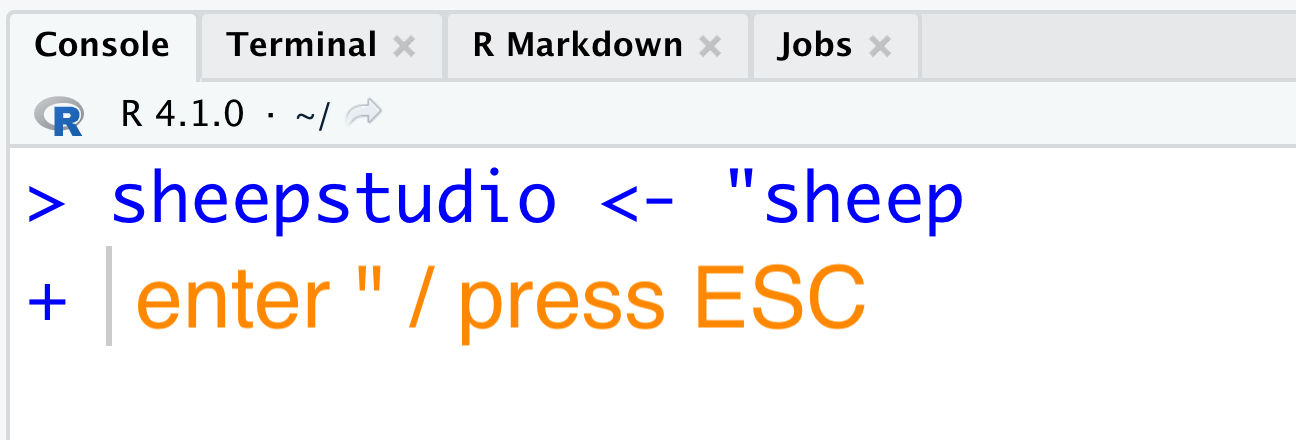
\includegraphics[width=0.7\linewidth]{pics/2quo} 

}

\caption{Miss the right quotation mark}\label{fig:quo}
\end{figure}

\end{infobox}

Similar to a numeric vector, you can use the \texttt{c()} function to combine several strings to create a character vector. You can verify the number of strings in the character vector by using \texttt{length()}, and \texttt{nchar()} can help you get the number of characters in each string.

\begin{Shaded}
\begin{Highlighting}[]
\NormalTok{animals }\OtherTok{\textless{}{-}} \FunctionTok{c}\NormalTok{(}\StringTok{"sheep@29"}\NormalTok{, }\StringTok{"pig$29"}\NormalTok{, }\StringTok{"monkey"}\NormalTok{)}
\NormalTok{animals}
\FunctionTok{length}\NormalTok{(animals)}
\FunctionTok{nchar}\NormalTok{(animals)}
\end{Highlighting}
\end{Shaded}

Note that if you have a vector consisted of numbers with surrounding double quotes, it is also a character vector. (``4'' and ``29'' are strings)

\begin{Shaded}
\begin{Highlighting}[]
\NormalTok{num\_vec }\OtherTok{\textless{}{-}} \FunctionTok{c}\NormalTok{(}\DecValTok{4}\NormalTok{, }\DecValTok{29}\NormalTok{)}
\NormalTok{char\_vec }\OtherTok{\textless{}{-}} \FunctionTok{c}\NormalTok{(}\StringTok{"4"}\NormalTok{, }\StringTok{"29"}\NormalTok{) }
\FunctionTok{class}\NormalTok{(num\_vec)}
\CommentTok{\#\textgreater{} [1] "numeric"}
\FunctionTok{class}\NormalTok{(char\_vec)}
\CommentTok{\#\textgreater{} [1] "character"}
\end{Highlighting}
\end{Shaded}

\textbf{\emph{b. Concatenate several strings into a single string}}

Next, we will introduce how to concatenate several strings into a single string. To do this, you can use the \texttt{paste()} function. First, let's create a character vector with four elements,

\begin{Shaded}
\begin{Highlighting}[]
\NormalTok{four\_strings }\OtherTok{\textless{}{-}} \FunctionTok{c}\NormalTok{(}\StringTok{"This"}\NormalTok{, }\StringTok{"is"}\NormalTok{, }\StringTok{"Sheep@29"}\NormalTok{, }\StringTok{"$Studio"}\NormalTok{)}
\FunctionTok{length}\NormalTok{(four\_strings) }\CommentTok{\#verify the number of strings}
\end{Highlighting}
\end{Shaded}

Then use \texttt{paste()} instead of \texttt{c()},

\begin{Shaded}
\begin{Highlighting}[]
\NormalTok{one\_long\_string }\OtherTok{\textless{}{-}} \FunctionTok{paste}\NormalTok{(}\StringTok{"This"}\NormalTok{, }\StringTok{"is"}\NormalTok{, }\StringTok{"Sheep@29"}\NormalTok{, }\StringTok{"$Studio"}\NormalTok{)}
\NormalTok{one\_long\_string}
\CommentTok{\#\textgreater{} [1] "This is Sheep@29 $Studio"}
\end{Highlighting}
\end{Shaded}

\begin{Shaded}
\begin{Highlighting}[]
\FunctionTok{class}\NormalTok{(one\_long\_string)}
\FunctionTok{length}\NormalTok{(one\_long\_string) }\CommentTok{\#verify the number of strings}
\end{Highlighting}
\end{Shaded}

From the results, you can see that \texttt{one\_long\_string} is a character vector with length 1, and the value of \texttt{one\_long\_string} is a single string with space between the individual strings.

You may notice that in \texttt{paste()}, the default separator between the individual strings is space. Actually you can change the separator by setting the \texttt{sep} argument in \texttt{paste()}. For example, you can separate the individual strings with comma,

\begin{Shaded}
\begin{Highlighting}[]
\NormalTok{comma }\OtherTok{\textless{}{-}} \FunctionTok{paste}\NormalTok{(}\StringTok{"This"}\NormalTok{, }\StringTok{"is"}\NormalTok{, }\StringTok{"Sheep@29"}\NormalTok{, }\StringTok{"$Studio"}\NormalTok{, }\AttributeTok{sep =} \StringTok{","}\NormalTok{) }
\NormalTok{comma}
\CommentTok{\#\textgreater{} [1] "This,is,Sheep@29,$Studio"}
\end{Highlighting}
\end{Shaded}

If you don't want to use a separator, you can use the \texttt{paste0()} function.

\begin{Shaded}
\begin{Highlighting}[]
\NormalTok{nosep }\OtherTok{\textless{}{-}} \FunctionTok{paste0}\NormalTok{(}\StringTok{"This"}\NormalTok{, }\StringTok{"is"}\NormalTok{, }\StringTok{"Sheep@29"}\NormalTok{, }\StringTok{"$Studio"}\NormalTok{) }
\NormalTok{nosep}
\CommentTok{\#\textgreater{} [1] "ThisisSheep@29$Studio"}
\end{Highlighting}
\end{Shaded}

If you would like to concatenate the strings of a vector into a longer string, you need to specify the \texttt{collapse} argument as the separator instead of \texttt{sep} in the \texttt{paste()} function.

\begin{Shaded}
\begin{Highlighting}[]
\FunctionTok{paste}\NormalTok{(four\_strings, }\AttributeTok{collapse =} \StringTok{""}\NormalTok{)}
\CommentTok{\#\textgreater{} [1] "ThisisSheep@29$Studio"}
\FunctionTok{paste}\NormalTok{(four\_strings, }\AttributeTok{collapse =} \StringTok{","}\NormalTok{)}
\CommentTok{\#\textgreater{} [1] "This,is,Sheep@29,$Studio"}
\FunctionTok{paste}\NormalTok{(four\_strings)                 }\DocumentationTok{\#\#doesn\textquotesingle{}t work without the collapse argument}
\CommentTok{\#\textgreater{} [1] "This"     "is"       "Sheep@29" "$Studio"}
\end{Highlighting}
\end{Shaded}

In addition to paste several strings into one long string, you can also use the \texttt{paste()} function paste two character vectors, where the pair of strings will be pasted elementwisely.

\begin{Shaded}
\begin{Highlighting}[]
\FunctionTok{paste}\NormalTok{(}\FunctionTok{c}\NormalTok{(}\StringTok{"July"}\NormalTok{, }\StringTok{"August"}\NormalTok{),  }\FunctionTok{c}\NormalTok{(}\StringTok{"2007"}\NormalTok{, }\StringTok{"2008"}\NormalTok{))}
\CommentTok{\#\textgreater{} [1] "July 2007"   "August 2008"}
\end{Highlighting}
\end{Shaded}

\textbf{\emph{c.~Change case}}

In character vectors, each string can contain both uppercase and lowercase letters. You can unify the cases of all letters inside a vector. Let's review the character vector \texttt{four\_strings} at first,

\begin{Shaded}
\begin{Highlighting}[]
\NormalTok{four\_strings }\OtherTok{\textless{}{-}} \FunctionTok{c}\NormalTok{(}\StringTok{"This"}\NormalTok{, }\StringTok{"is"}\NormalTok{, }\StringTok{"Sheep@29"}\NormalTok{, }\StringTok{"$Studio"}\NormalTok{)}
\NormalTok{four\_strings}
\CommentTok{\#\textgreater{} [1] "This"     "is"       "Sheep@29" "$Studio"}
\end{Highlighting}
\end{Shaded}

Then use the \texttt{tolower()} function to convert all letters to lower case,

\begin{Shaded}
\begin{Highlighting}[]
\FunctionTok{tolower}\NormalTok{(four\_strings)}
\CommentTok{\#\textgreater{} [1] "this"     "is"       "sheep@29" "$studio"}
\end{Highlighting}
\end{Shaded}

The opposite function of \texttt{tolower()} is \texttt{toupper()}, which converts all letters to upper case,

\begin{Shaded}
\begin{Highlighting}[]
\FunctionTok{toupper}\NormalTok{(four\_strings)}
\CommentTok{\#\textgreater{} [1] "THIS"     "IS"       "SHEEP@29" "$STUDIO"}
\end{Highlighting}
\end{Shaded}

\hypertarget{logical-vector}{%
\subsection{Logical vector}\label{logical-vector}}

So far we have created several numeric vectors and character vectors. Some vectors have names, and some do not. You can see all the \textbf{named objects} by using the \texttt{ls()} function.

\begin{Shaded}
\begin{Highlighting}[]
\FunctionTok{ls}\NormalTok{()}
\CommentTok{\#\textgreater{}  [1] "animals"         "char\_vec"        "comma"           "four\_strings"   }
\CommentTok{\#\textgreater{}  [5] "nosep"           "num\_vec"         "one\_long\_string" "sheepstudio"    }
\CommentTok{\#\textgreater{}  [9] "x1"              "x2"              "y1"              "y2"             }
\CommentTok{\#\textgreater{} [13] "y3"              "z1"}
\end{Highlighting}
\end{Shaded}

As introduced in Section \ref{Object-Assignment}, another way to check the named objects is via the environment panel as shown in Figure \ref{fig:enviro}.

\begin{figure}

{\centering 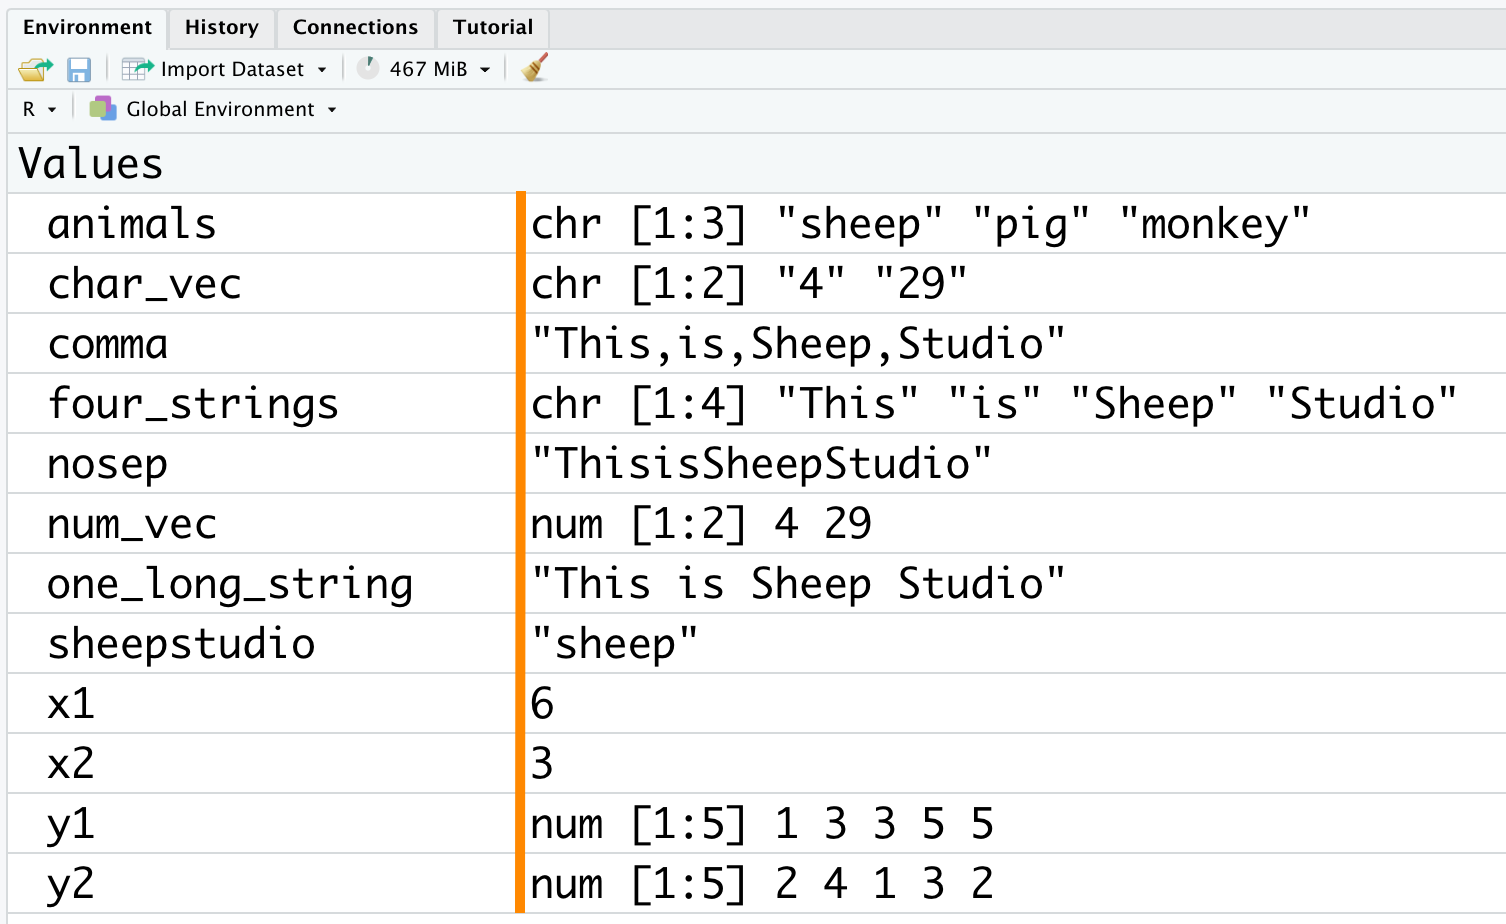
\includegraphics[width=0.7\linewidth]{pics/2enviro} 

}

\caption{Environment}\label{fig:enviro}
\end{figure}

We can see that the environment panel has two columns, with the first column showing the list of object names, and the second column showing the corresponding information for each object. The information includes the vector type (\emph{chr} is short for character and \emph{num} is short for numeric), the vector length, and the first few values of the vector. Note that if the vector is of length 1 (for example \texttt{x1}), the environment will not show the type or the length.

\begin{infobox}{caution}
By now you have created several objects, and you will find that the objects will not be saved in R if you don't assign their values to names, for example, the results of \texttt{x1\ +\ x2} and \texttt{y1\ +\ y2} are not shown in the environment.

\end{infobox}

Before introducing the \emph{logical vector}, let's first learn a function called \texttt{is.numeric()}, which checks whether a vector is of numeric type,

\begin{Shaded}
\begin{Highlighting}[]
\FunctionTok{is.numeric}\NormalTok{(y1) }\CommentTok{\#Is y1 of numeric type?}
\CommentTok{\#\textgreater{} [1] TRUE}
\end{Highlighting}
\end{Shaded}

Similar to \texttt{is.numeric()}, you can also use \texttt{is.character()} function to check if the given vector is of character type.

\begin{Shaded}
\begin{Highlighting}[]
\FunctionTok{is.character}\NormalTok{(y1) }\CommentTok{\#Is y1 of character type?}
\CommentTok{\#\textgreater{} [1] FALSE}
\end{Highlighting}
\end{Shaded}

You may notice that results are \texttt{TRUE} or \texttt{FALSE} from the above codes. Actually, \textbf{logical vectors} are vectors that only use \texttt{TRUE} or \texttt{FALSE} as values. Note that \texttt{TRUE} and \texttt{FALSE} are logical constants in R. Similarly, you can use \texttt{is.logical()} to check if the vector is of logical type, or you can use \texttt{class()} to find out the exact type.

\begin{Shaded}
\begin{Highlighting}[]
\NormalTok{logic1 }\OtherTok{\textless{}{-}} \FunctionTok{c}\NormalTok{(}\ConstantTok{TRUE}\NormalTok{, }\ConstantTok{FALSE}\NormalTok{, }\ConstantTok{TRUE}\NormalTok{) }\CommentTok{\#you can also use the c() function to create a logical vector}
\FunctionTok{is.logical}\NormalTok{(logic1)}
\FunctionTok{class}\NormalTok{(logic1)}
\end{Highlighting}
\end{Shaded}

You can also use \texttt{T} to represent \texttt{TRUE} and \texttt{F} to represent \texttt{FALSE} in logical vectors.

\begin{Shaded}
\begin{Highlighting}[]
\NormalTok{logic2 }\OtherTok{\textless{}{-}} \FunctionTok{c}\NormalTok{(T, F, F)}
\FunctionTok{is.logical}\NormalTok{(logic2)}
\FunctionTok{class}\NormalTok{(logic2)}
\end{Highlighting}
\end{Shaded}

It is worth to point out that you don't want to put a pair of double quotes around \texttt{TRUE} or \texttt{FALSE} when you use them as logical values. If you do that, a character vector will be generated instead.

\begin{Shaded}
\begin{Highlighting}[]
\NormalTok{char }\OtherTok{\textless{}{-}} \FunctionTok{c}\NormalTok{(}\StringTok{"TRUE"}\NormalTok{, }\StringTok{"FALSE"}\NormalTok{, }\StringTok{"TRUE"}\NormalTok{)}
\FunctionTok{is.logical}\NormalTok{(char)}
\end{Highlighting}
\end{Shaded}

Note that the keywords \texttt{TRUE} and \texttt{FALSE} are case sensitive, and all letters inside them need to be in \textbf{upper case}. If you change any letter to the lower case, you will get an error, because \texttt{True} is neither a logical constant nor a defined object.

\begin{Shaded}
\begin{Highlighting}[]
\NormalTok{tlogic }\OtherTok{\textless{}{-}}\NormalTok{ True}
\CommentTok{\#\textgreater{} Error in eval(expr, envir, enclos): object \textquotesingle{}True\textquotesingle{} not found}
\end{Highlighting}
\end{Shaded}

\hypertarget{exercises-4}{%
\subsection{Exercises}\label{exercises-4}}

\begin{enumerate}
\def\labelenumi{\arabic{enumi}.}
\item
  Write R code to create a numeric vector named \texttt{vec\_1} with values \texttt{7\ 24\ 8\ \ 26}, get its length, and find out its type.
\item
  Write R code to create a character vector named \texttt{char\_1} with values \texttt{"I"}, \texttt{"am"}, \texttt{"learning"}, \texttt{"R!"}, get its length, find out its type, and concatenate the vector into a single string with space as the separator.
\item
  For the \texttt{char\_1} defined in Q2, find the number of characters in each string, and convert each string to upper case.
\item
  Create a length-2 logical vector representing whether \texttt{vec\_1} and \texttt{char\_1} are of character type.
\end{enumerate}

\hypertarget{intro-logi-vector}{%
\section{Introduction to Logical Vectors}\label{intro-logi-vector}}

Having learning numeric vectors and character vectors, it is time to master \textbf{logical vectors}, which is another type of atomic vectors, containing only logical values.

\hypertarget{create-logical-vector}{%
\subsection{Logical vectors: creation by comparisons and class}\label{create-logical-vector}}

A \textbf{logical vector} is an atomic vector containing only logical values, namely \texttt{TRUE} and \texttt{FALSE}. Logical vectors are most often encountered when we want to check whether a comparison statement is true or false.

\textbf{\emph{a. Compare two vectors of the same length}}

If two vectors are of the same length, the comparison is done elementwisely, just like the arithmetic operations in Section \ref{vector}.

You can create a numeric vector \texttt{x} with value \texttt{3}, and compare it to another numeric vector \texttt{2} to find out whether the value of \texttt{x} is smaller than 2 or not.

\begin{Shaded}
\begin{Highlighting}[]
\NormalTok{x }\OtherTok{\textless{}{-}} \DecValTok{3}
\NormalTok{x }\SpecialCharTok{\textless{}} \DecValTok{2}
\CommentTok{\#\textgreater{} [1] FALSE}
\NormalTok{x }\SpecialCharTok{\textgreater{}} \DecValTok{1}
\CommentTok{\#\textgreater{} [1] TRUE}
\end{Highlighting}
\end{Shaded}

The value of \texttt{x\ \textless{}\ 2} is \texttt{FALSE} since 3 is not smaller than 2, and the value of \texttt{x\ \textgreater{}\ 1} is \texttt{TRUE} since 3 is not larger than 1.

There are a few other commonly useful operators for doing comparisons.

\begin{Shaded}
\begin{Highlighting}[]
\NormalTok{x }\SpecialCharTok{\textless{}} \DecValTok{2}      \CommentTok{\#less than}
\CommentTok{\#\textgreater{} [1] FALSE}
\NormalTok{x }\SpecialCharTok{\textless{}=} \DecValTok{2}     \CommentTok{\#less than or equal to}
\CommentTok{\#\textgreater{} [1] FALSE}
\NormalTok{x }\SpecialCharTok{\textgreater{}} \DecValTok{1}      \CommentTok{\#bigger than}
\CommentTok{\#\textgreater{} [1] TRUE}
\NormalTok{x }\SpecialCharTok{\textgreater{}=} \DecValTok{1}     \CommentTok{\#bigger than or equal to}
\CommentTok{\#\textgreater{} [1] TRUE}
\NormalTok{x }\SpecialCharTok{==} \DecValTok{3}     \CommentTok{\#equal to}
\CommentTok{\#\textgreater{} [1] TRUE}
\CommentTok{\#x = 3     \#assignment operator}
\NormalTok{x }\SpecialCharTok{!=} \DecValTok{3}     \CommentTok{\#not equal to}
\CommentTok{\#\textgreater{} [1] FALSE}
\end{Highlighting}
\end{Shaded}

Note that if you want to check whether two vectors are equal, you have to use \textbf{two equal signs} (with not space in-between) as a single operator, which is \texttt{==}, to do comparisons. If only one equal sign is used, it would work as an assignment operator. In addition, you can use an exclamation mark together with a equal sign, which is \texttt{!=}, to find out whether two vectors are not equal.

Let's first create a numeric vector \texttt{x1} and make some comparisons.

\begin{Shaded}
\begin{Highlighting}[]
\NormalTok{x1 }\OtherTok{\textless{}{-}} \DecValTok{6}                  
\NormalTok{x1 }\SpecialCharTok{\textgreater{}} \DecValTok{5}
\CommentTok{\#\textgreater{} [1] TRUE}
\NormalTok{x1 }\SpecialCharTok{\textless{}} \DecValTok{3}
\CommentTok{\#\textgreater{} [1] FALSE}
\end{Highlighting}
\end{Shaded}

The value of \texttt{x1\ \textgreater{}\ 5} is \texttt{TRUE} since 6 \textgreater{} 5, and the value of \texttt{x1\ \textless{}\ 3} is \texttt{FALSE} since 5 is not smaller than 3.

In addition to making comparisons involving a vector of length 1, you can also do it with vectors containing more than 1 elements.

When we make comparisons between two vectors of more than 1 elements, R will make a elementwise comparison just like the arithmetic operations between two numeric vectors.

\begin{Shaded}
\begin{Highlighting}[]
\NormalTok{x2 }\OtherTok{\textless{}{-}} \FunctionTok{c}\NormalTok{(}\DecValTok{1}\NormalTok{, }\DecValTok{2}\NormalTok{, }\DecValTok{6}\NormalTok{)}
\NormalTok{x3 }\OtherTok{\textless{}{-}} \FunctionTok{c}\NormalTok{(}\DecValTok{2}\NormalTok{, }\DecValTok{2}\NormalTok{, }\DecValTok{4}\NormalTok{)}
\NormalTok{x2 }\SpecialCharTok{\textless{}=}\NormalTok{ x3}
\CommentTok{\#\textgreater{} [1]  TRUE  TRUE FALSE}
\end{Highlighting}
\end{Shaded}

You can check that the logical values correspond to the comparisons \texttt{1\ \textless{}=\ 2}, \texttt{2\ \textless{}=\ 2}, and \texttt{6\ \textless{}=\ 4}.

Also similar to the arithmetic operations on numeric vectors, the recycling rule also applies for comparisons when the two vectors in action are not of the same length.

\begin{Shaded}
\begin{Highlighting}[]
\NormalTok{x3 }\SpecialCharTok{!=} \DecValTok{2}
\CommentTok{\#\textgreater{} [1] FALSE FALSE  TRUE}
\end{Highlighting}
\end{Shaded}

Moving on, you may wonder, can a numeric vector contain more than one values? The answer is a big YES! In R, you can use the \texttt{c()} function (\texttt{c} is short for combine) to combine elements into a numeric vector.

\begin{Shaded}
\begin{Highlighting}[]
\FunctionTok{c}\NormalTok{(}\DecValTok{1}\NormalTok{, }\DecValTok{3}\NormalTok{, }\DecValTok{3}\NormalTok{, }\DecValTok{5}\NormalTok{, }\DecValTok{5}\NormalTok{)          }\CommentTok{\#use c() to combine elements into a numeric vector of length 5}
\CommentTok{\#\textgreater{} [1] 1 3 3 5 5}
\NormalTok{y1 }\OtherTok{\textless{}{-}} \FunctionTok{c}\NormalTok{(}\DecValTok{1}\NormalTok{, }\DecValTok{3}\NormalTok{, }\DecValTok{3}\NormalTok{, }\DecValTok{5}\NormalTok{, }\DecValTok{5}\NormalTok{)    }\CommentTok{\#y1 is a numeric vector of length 5}
\NormalTok{y1                        }\CommentTok{\#check the value of y1}
\CommentTok{\#\textgreater{} [1] 1 3 3 5 5}
\FunctionTok{length}\NormalTok{(y1)                }\CommentTok{\#length of y1}
\CommentTok{\#\textgreater{} [1] 5}
\end{Highlighting}
\end{Shaded}

In this example, you have created a length-5 object using the \texttt{c()} function with arguments being the five elements separated by comma. Since the value of each element is a number, the object is a numeric vector.

Notice that the second and third elements in \texttt{y1} have the same value 3. Similar to \texttt{x1}, you can verify the contents of \texttt{y1} and check the length of it via the \texttt{length()} function.

\begin{infobox}{caution}

When you assign several values to a name, the order of the values will not change after assignment. If you create two numeric vectors containing the same numbers but in different orders, the two vectors will maintain the specified orders. For example,

\begin{Shaded}
\begin{Highlighting}[]
\NormalTok{y2 }\OtherTok{\textless{}{-}} \FunctionTok{c}\NormalTok{(}\DecValTok{1}\NormalTok{, }\DecValTok{3}\NormalTok{, }\DecValTok{5}\NormalTok{, }\DecValTok{7}\NormalTok{, }\DecValTok{9}\NormalTok{)    }
\NormalTok{y2                        }
\CommentTok{\#\textgreater{} [1] 1 3 5 7 9}
\NormalTok{y3 }\OtherTok{\textless{}{-}} \FunctionTok{c}\NormalTok{(}\DecValTok{9}\NormalTok{, }\DecValTok{7}\NormalTok{, }\DecValTok{5}\NormalTok{, }\DecValTok{3}\NormalTok{, }\DecValTok{1}\NormalTok{)    }
\NormalTok{y3}
\CommentTok{\#\textgreater{} [1] 9 7 5 3 1}
\end{Highlighting}
\end{Shaded}

\end{infobox}

In addition to using numbers inside the \texttt{c()} function, you can also use several numeric vectors as the arguments to create a longer vector. The new. longer vector will combine the input numeric vectors in the given order.

\begin{Shaded}
\begin{Highlighting}[]
\FunctionTok{c}\NormalTok{(x1, y1)          }\CommentTok{\#use c() to combine several numeric vectors into one numeric vector}
\CommentTok{\#\textgreater{} [1] 6 1 3 3 5 5}
\NormalTok{z1 }\OtherTok{\textless{}{-}} \FunctionTok{c}\NormalTok{(x1, y1)}
\NormalTok{z1}
\CommentTok{\#\textgreater{} [1] 6 1 3 3 5 5}
\FunctionTok{length}\NormalTok{(z1)}
\CommentTok{\#\textgreater{} [1] 6}
\end{Highlighting}
\end{Shaded}

For any R object, you can use the function \texttt{class()} to check its \textbf{class}. A class can be thought of as a ``type,'' providing a description about the object, and determines what functions can be applied to it.

\begin{Shaded}
\begin{Highlighting}[]
\FunctionTok{class}\NormalTok{(x1)}
\CommentTok{\#\textgreater{} [1] "numeric"}
\FunctionTok{class}\NormalTok{(y1)}
\CommentTok{\#\textgreater{} [1] "numeric"}
\FunctionTok{class}\NormalTok{(z1)}
\CommentTok{\#\textgreater{} [1] "numeric"}
\end{Highlighting}
\end{Shaded}

From the results, you can see that \texttt{x1}, \texttt{y1}, and \texttt{z1} are all numeric, which is the reason why they are called \emph{numeric vectors}.

\hypertarget{numeric-vectors-access-and-modify-elements-1}{%
\subsection{Numeric vectors: access and modify elements}\label{numeric-vectors-access-and-modify-elements-1}}

To \textbf{access an element} from a vector, you can use the vector name followed by a pair of \texttt{{[}} and \texttt{{]}}containing the index of the desired element. Let's see some examples.

\begin{Shaded}
\begin{Highlighting}[]
\NormalTok{y1[}\DecValTok{2}\NormalTok{]     }\CommentTok{\#access the second element of y1}
\CommentTok{\#\textgreater{} [1] 3}
\NormalTok{y2[}\DecValTok{3}\NormalTok{]     }\CommentTok{\#access the third element of y2}
\CommentTok{\#\textgreater{} [1] 5}
\end{Highlighting}
\end{Shaded}

You can also \textbf{modify} a particular element of a vector by using the \emph{assignment operator} with the access expression on the left and the new value on the right.

\begin{Shaded}
\begin{Highlighting}[]
\NormalTok{y1               }\CommentTok{\#the current value of y1}
\CommentTok{\#\textgreater{} [1] 1 3 3 5 5}
\NormalTok{y1[}\DecValTok{2}\NormalTok{] }\OtherTok{\textless{}{-}} \DecValTok{100}     \CommentTok{\#modify the second element of y1 to 100}
\NormalTok{y1               }\CommentTok{\#the new value of y1}
\CommentTok{\#\textgreater{} [1]   1 100   3   5   5}
\end{Highlighting}
\end{Shaded}

As you can see here, the second element of \texttt{y1} is modified to 100, which is reflected via checking the value of \texttt{y1}.

Let's look at another example where we want to modify the third element of \texttt{y2} to be twice as much as the fourth element of \texttt{y1}.

\begin{Shaded}
\begin{Highlighting}[]
\NormalTok{y2                     }\CommentTok{\#the current value of y2}
\CommentTok{\#\textgreater{} [1] 1 3 5 7 9}
\NormalTok{y2[}\DecValTok{3}\NormalTok{] }\OtherTok{\textless{}{-}}\NormalTok{ y1[}\DecValTok{4}\NormalTok{] }\SpecialCharTok{*} \DecValTok{2}     \CommentTok{\#modify the third element of y2}
\NormalTok{y2                     }\CommentTok{\#the new value of y2}
\CommentTok{\#\textgreater{} [1]  1  3 10  7  9}
\end{Highlighting}
\end{Shaded}

\hypertarget{numeric-vectors-operations-and-recycling-rule-1}{%
\subsection{Numeric vectors: operations and recycling rule}\label{numeric-vectors-operations-and-recycling-rule-1}}

Since numeric vectors are purely made of numbers, you can do \textbf{arithmetic operations} between them, just like the fancy calculator in Section \ref{Calculator}. If two vectors are of the \textbf{same length}, the operation is done \textbf{element-wisely}. In other words, R will perform the operation between elements in the same index of different vectors. First, let's create another vector \texttt{x2} of length 1 and compute the sum of \texttt{x1} and \texttt{x2}. Also recall that we've previously assigned x1 to a length-1 numeric vector of value 6.

\begin{Shaded}
\begin{Highlighting}[]
\NormalTok{x1}
\CommentTok{\#\textgreater{} [1] 6}
\NormalTok{x2 }\OtherTok{\textless{}{-}} \DecValTok{3}
\NormalTok{x1 }\SpecialCharTok{+}\NormalTok{ x2}
\CommentTok{\#\textgreater{} [1] 9}
\end{Highlighting}
\end{Shaded}

Similarly, you can create another vector \texttt{y2} of the same length as vector \texttt{y1}. Then, you can do operations between \texttt{y1} and \texttt{y2}.

\begin{Shaded}
\begin{Highlighting}[]
\NormalTok{y1}
\CommentTok{\#\textgreater{} [1]   1 100   3   5   5}
\NormalTok{y2 }\OtherTok{\textless{}{-}} \FunctionTok{c}\NormalTok{(}\DecValTok{2}\NormalTok{, }\DecValTok{4}\NormalTok{, }\DecValTok{1}\NormalTok{, }\DecValTok{3}\NormalTok{, }\DecValTok{2}\NormalTok{)}
\NormalTok{y1 }\SpecialCharTok{*}\NormalTok{ y2}
\CommentTok{\#\textgreater{} [1]   2 400   3  15  10}
\end{Highlighting}
\end{Shaded}

The result is yet another length-5 vector. To check the calculation was indeed done element-wisely, you can verify that the value of the first element is \(1 * 2 = 2\), and value of the second element is \(100 * 4 = 400\), etc.

Since the calculation is done element-wisely, we normally would want the two vectors to have the same length. However, there is an important \textbf{recycling} rule in R, which is quite useful and enables us to write simpler code. Specifically, if one vector is shorter than the other vector, R will \textbf{recycle} (repeat) the shorter vector until it matches in length with the longer one. This recycling is most often used for an operation between a \textbf{length\textgreater1} vector and a \textbf{length-1} vector. Let's see an example.

\begin{Shaded}
\begin{Highlighting}[]
\NormalTok{y1 }\SpecialCharTok{+}\NormalTok{ x1}
\CommentTok{\#\textgreater{} [1]   7 106   9  11  11}
\end{Highlighting}
\end{Shaded}

From the result, you can see that \texttt{x1} is recycled five times to match in length with \texttt{y1}. Consequently, each element in \texttt{y1} is added by 6.

The followings are a few additional examples you can try.

\begin{Shaded}
\begin{Highlighting}[]
\NormalTok{y1 }\SpecialCharTok{*}\NormalTok{ x2}
\NormalTok{y1 }\SpecialCharTok{/} \DecValTok{5}
\NormalTok{y2 }\SpecialCharTok{{-}}\NormalTok{ x1}
\end{Highlighting}
\end{Shaded}

\hypertarget{storage-type}{%
\subsection{Numeric vectors: storage types (doubles and intergers)}\label{storage-type}}

Now, it is time to learn how numeric vectors are stored in R. To find the \textbf{internal storage type} of an R object, you can use the \texttt{typeof()} function.

\begin{Shaded}
\begin{Highlighting}[]
\NormalTok{my\_double }\OtherTok{\textless{}{-}} \FunctionTok{c}\NormalTok{(}\DecValTok{1}\NormalTok{, }\DecValTok{3}\NormalTok{, }\DecValTok{4}\NormalTok{)}
\FunctionTok{typeof}\NormalTok{(my\_double)         }\CommentTok{\#internal storage type}
\CommentTok{\#\textgreater{} [1] "double"}
\end{Highlighting}
\end{Shaded}

We can see that the internal storage type of \texttt{my\_num} is \textbf{double}, meaning that \texttt{my\_num} is stored as a \textbf{double precision} numeric value. Looking at the values of \texttt{my\_num}, it is easy to see that they are all integers. In fact, R stores numeric vectors as double precision vectors by default. That being said, you can always store the integers in a \textbf{integer type}, which offers great memory savings compared to doubles. The tricky part is that you usually need to explicitly tell R that you are storing them as integers.

To create an integer vector, you can still use the \texttt{c()} function with the integers separated by comma as arguments. However, you need to put an ``L'' after each integer. Let's create an integer and check its storage type as well as its class.

\begin{Shaded}
\begin{Highlighting}[]
\NormalTok{my\_int }\OtherTok{\textless{}{-}} \FunctionTok{c}\NormalTok{(1L, 3L, 4L)}
\FunctionTok{typeof}\NormalTok{(my\_int)}
\CommentTok{\#\textgreater{} [1] "integer"}
\FunctionTok{class}\NormalTok{(my\_int)}
\CommentTok{\#\textgreater{} [1] "integer"}
\end{Highlighting}
\end{Shaded}

You can see that \texttt{my\_int} is indeed of \texttt{integer} type, with the \texttt{class} of it being \texttt{integer} as well.

It is also worth noting that the displaying value of \texttt{my\_double} and \texttt{my\_int} are the same, though they are stored differently in the memory.

\begin{Shaded}
\begin{Highlighting}[]
\NormalTok{my\_double}
\CommentTok{\#\textgreater{} [1] 1 3 4}
\NormalTok{my\_int}
\CommentTok{\#\textgreater{} [1] 1 3 4}
\end{Highlighting}
\end{Shaded}

\begin{infobox}{caution}
Despite the differences between integers and doubles, you can usually ignore their differences unless you are working on a very big data set. R will automatically convert objects between integers and doubles when necessary.

\end{infobox}

\hypertarget{numeric-vectors-printing-1}{%
\subsection{Numeric vectors: printing}\label{numeric-vectors-printing-1}}

Now, you have already learned to run the object name to reveal its value. Let's try to type \texttt{pi}, which is an internal constant available for use.

\begin{Shaded}
\begin{Highlighting}[]
\NormalTok{pi}
\CommentTok{\#\textgreater{} [1] 3.141593}
\end{Highlighting}
\end{Shaded}

As you can see from the output, R prints out 7 significant digits by default, though in fact we need infinitely many digits to faithfully represent \texttt{pi}. To print out an object with a customized significant digit number, you can use the \texttt{print()} function that contains useful argument called \texttt{digits}, which controls the minimal number of significant digits. Let's see the following examples.

\begin{Shaded}
\begin{Highlighting}[]
\FunctionTok{print}\NormalTok{(pi)}
\CommentTok{\#\textgreater{} [1] 3.141593}
\FunctionTok{print}\NormalTok{(pi, }\AttributeTok{digits =} \DecValTok{3}\NormalTok{)            }\CommentTok{\#print pi for 3 significant digits}
\CommentTok{\#\textgreater{} [1] 3.14}
\FunctionTok{print}\NormalTok{(pi, }\AttributeTok{digits =} \DecValTok{16}\NormalTok{)           }\CommentTok{\#print pi for 16 significant digits}
\CommentTok{\#\textgreater{} [1] 3.141592653589793}
\FunctionTok{print}\NormalTok{(}\FunctionTok{c}\NormalTok{(pi, }\FunctionTok{exp}\NormalTok{(}\DecValTok{1}\NormalTok{), }\FunctionTok{log}\NormalTok{(}\DecValTok{2}\NormalTok{)), }\AttributeTok{digits =} \DecValTok{4}\NormalTok{)}
\CommentTok{\#\textgreater{} [1] 3.1416 2.7183 0.6931}
\end{Highlighting}
\end{Shaded}

As you can imagine, the \texttt{print()} function will be very useful in creating tables that look more streamlined.

\hypertarget{exercises-5}{%
\subsection{Exercises}\label{exercises-5}}

Write R code to complete the following tasks.

\begin{enumerate}
\def\labelenumi{\arabic{enumi}.}
\item
  Create a numeric vector named \texttt{vec\_1} with values \((2, 4, 6, 8)\), get its length, find out its class, and get its storage type.
\item
  For the numeric vector \texttt{vec\_2\ \textless{}-\ c(1,\ 3,\ 7,\ 10)}, get the value of the 3rd element, multiple the 3rd element by 5, and verify the change.
\item
  Create a vector \texttt{vec\_3} where each element is twice the corresponding element in \texttt{vec\_1} minus half the corresponding element in \texttt{vec\_2}.
\item
  Create an integer vector \texttt{int\_1} that contains integers \((2, 4, 6, 8)\). Check its class and storage type.
\item
  Print out the vector \((e, e^2, e^3)\) with 5 significant digits.
\end{enumerate}

  \bibliography{book.bib,packages.bib}

\end{document}
